\documentclass[12pt, a4paper, twoside]{report}
\usepackage[a4paper, top=1in, bottom=1in, left=.8in, right=.8in]{geometry}
\usepackage{amsmath}
\usepackage{graphicx}
\usepackage{subcaption}
\usepackage{booktabs}
\usepackage[table,xcdraw]{xcolor}
\usepackage{pgfplots}
\pgfplotsset{compat=1.15}
\setlength{\parindent}{0em}
\setlength{\parskip}{1em}
\usepackage{floatrow}
\newfloatcommand{capbtabbox}{table}[][\FBwidth]
\usepackage{enumitem}
\usepackage{float}
\usepackage{minted}
\usepackage[titletoc]{appendix}
\usepackage[acronym, nonumberlist]{glossaries}

\makeglossaries
\newacronym{hmm}{HMM}{Hidden Markov Model}
\newacronym{gmm}{GMM}{Gaussian Mixture Model}
\newacronym{asr}{ASR}{Automatic Speech Recognition}
\newacronym{dnn}{DNN}{Deep Neural Network}
\newacronym{lpc}{LPC}{Linear Predictive Coding}
\newacronym{mfcc}{MFCC}{Mel-Frequency Cepstral Coefficients}
\newacronym{dwt}{DWT}{Discrete Wavelet Transform}
\newacronym{dtw}{DTW}{Dynamic Time Warping}
\newacronym{ipa}{IPA}{International Phonetic Alphabet}
\newacronym{zcr}{ZCR}{Zero-Crossing Rate}
\newacronym{pdf}{PDF}{Probability Density Function}
\newacronym{ste}{STE}{Short Time Energy}
\newacronym{fft}{FFT}{Fast Fourier Transform}
\newacronym{dct}{DCT}{Discrete Cosine Transform}
\newacronym{em}{EM}{Expectation Maximization}
\newacronym{nn}{NN}{Neural Network}
\newacronym{usart}{USART}{Universal Synchronous and Asynchronous Receiver-Transmitter}
\newacronym{ttl}{TTL}{Transistor-to-Transistor Logic}
\newacronym{gpio}{GPIO}{General-Purpose Input/Output}

\begin{document}

\begin{titlepage}
	\begin{flushright}
		{\scshape Alexandria University\\}
		{\huge Speech Recognition for Automated Systems\par}
	\end{flushright}
	\vfill
	{\Large\itshape
		Ahmed B. Ghareeb\par
		Ahmed F. Abdel-Aal\par
		Khaled M. Mashaly\par
		Kareem M. El-Far\par
		Kareem M. Emam\par
		Moemen M. Youssof\par
		Marco A. Bekhiet\par
		Magdy I. Moussa\par
		Mohammed A. Seleem\par
		Mahmoud M. El-Tahan\par
	}
	\vspace{1cm}
	supervised by\\ \\
	{\Large\itshape Dr.~Mohamed Moselhy}
\end{titlepage}

\begin{abstract}
Abstract goes here...
\end{abstract}

\printglossary[type=\acronymtype]

\tableofcontents

\chapter{Introduction}
\section{An overview of Speech Recognition}
Speech recognition is a technology that enables machines to capture the words spoken by a human with a help of microphone. These words are later recognized by speech recognizer, and in the end, system outputs the recognized words. The process of speech recognition consists of different steps that will be discussed in the following chapters one by one.
\par
An ideal situation in the process of speech recognition is that, a speech recognition engine recognizes all words uttered by a human but, practically the performance of a speech recognition engine depends on number of factors. Vocabularies, multiple users and noisy environment are the major factors that are counted in as the depending factors for a speech recognition engine.
\section{History}
In the 1950s Bell Laboratories successfully build an isolated digit recognition system for a single speaker. Early recognition systems used intuitive techniques which were based on measuring formant frequencies but only after the introduction of statistical modelling in the 1980s speech recognition systems started to have more practical uses. Even nowadays the Hidden Markov Models (\acrshort{hmm}s) are the most popular foundation for Automatic Speech Recognition (\acrshort{asr}) systems though the Deep Neural Networks (\acrshort{dnn}) has begun to be more common in the past decade.
\section{Classification Of Speech Recognition Systems}
Speech recognition systems can be separated in several different classes by describing the type of speech utterance, type of speaker model, type of channel and the type of vocabulary that they have the ability to recognize. Speech recognition is becoming more complex and a challenging task because of this variability in the signal. These challenges are briefly explained below.
\subsection{Types of speech recognition}
An utterance is the vocalization (speaking) of a word or words that represent a single meaning to the computer. Utterances can be a single word, a few words, a sentence, or even multiple sentences. Types of speech utterance are:
\begin{enumerate}[label=\textbf{\Roman*.}]
\item \textbf{Isolated Words}\\
Isolated word recognizers usually require each utterance to have quiet (lack of an audio signal) on both sides of the sample window. It accepts single words or single utterance at a time. These systems have ``Listen/Not-Listen'' states, where they require the speaker to wait between utterances (usually doing processing during the pauses). Isolated Utterance might be a better name for this class.
\item \textbf{Connected Words}\\
Connected word systems are similar to isolated words, but allow separate utterances to be ``run-together'' with a minimal pause between them.
\item \textbf{Continuous Speech}\\
Continuous speech recognizers allow users to speak almost naturally, while the computer determines the content. Recognizers with continuous speech capabilities are some of the most difficult to create because they utilize special methods to determine utterance boundaries. 
\item \textbf{Spontaneous Speech}\\
At a basic level, it can be thought of as speech that is natural sounding. System with spontaneous speech ability should be able to handle a variety of natural speech features such as words being run together.
\end{enumerate}

\subsection{Speaker Model Types}
Speech recognition system is broadly classified into two main categories based on speaker models namely speaker dependent and speaker independent.
\begin{enumerate}[label=\textbf{\Roman*.}]
\item \textbf{Speaker dependent models}\\
Speaker dependent systems are designed for a specific speaker. They are generally more accurate for the particular speaker, but much less accurate for other speakers. These systems are usually easier to develop, cheaper and more accurate, but not as flexible as speaker independent systems. 
\item \textbf{Speaker independent models}\\
Speaker independent systems are designed for variety of speakers. It recognizes the speech patterns of a large group of people. This system is most difficult to develop, most expensive and offers less accuracy than speaker dependent systems. However, they are more flexible.
\end{enumerate}
\subsection{Size of Vocabulary}
The size of vocabulary of a speech recognition system affects the complexity, processing requirements and the accuracy of the system. Some applications only require a few words (e.g. numbers only), others require very large dictionaries. In \acrshort{asr} systems the types of vocabularies can be classified as follows.
\begin{enumerate}
\item Small vocabulary - tens of words
\item Medium vocabulary - hundreds of words
\item Large vocabulary - thousands of words
\item Very-large vocabulary - tens of thousands of words
\item Out-of-Vocabulary- Mapping a word from the vocabulary into the unknown word.
\end{enumerate}
\section{Speech Recognition Process}

\begin{figure}[ht]
	\centering
	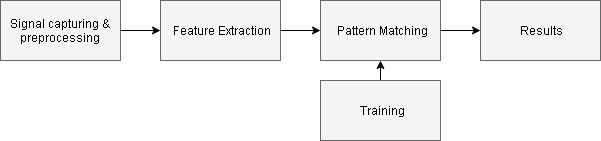
\includegraphics[width=1\textwidth]
	{images/chapter1/chapter1}
	\caption{general speech recognition system.}
	\label{fig:chapter1}
\end{figure}

\subsection{Preprocessing}
In Automatic Speech Recognition system the first phase is pre-processing phase. Moreover, Pre-Processing of Speech is very important in the applications where silence or ambient noise is completely undesirable. Voice activity detection is a well-known technique adopted for many years in preprocessing of speech signal, Noise canceling, pre-emphasis and dimensionality reduction of speech facilitates the system to be computationally more efficient.
\subsection{Feature Extraction}
Speech feature extraction is responsible for transformation of the speech signals into stream of feature vectors coefficients which contains only that information which is required for the identification of a given utterance. As every speech has different unique attributes contained in spoken words these attributes can be extracted from a wide range of feature extraction techniques and can be employed for speech recognition task. But extracted feature should meet certain criteria while dealing with the speech signal such as: extracted speech features should be measured easily, extracted features should be consistent with time, and features should be robust to noise and environment. The feature vector of speech signals are typically extracted using spectral analysis techniques such as \acrfull{mfcc}, \acrfull{lpc}, \acrfull{dwt}.
\subsection{Classification}
Once a voice sample has been converted to a series of feature vectors it can be fed into the model to determine who or what has been spoken. This is done by building a model using the extracted features. In speech recognition process we can use the following modelling approaches:
\begin{itemize}
\item {\bfseries Acoustic-Phonetic approach:} The basic principle that this approach follows is identifying the speech signals and then providing these speech signals with. Thus the acoustic phonetic approach postulates that there exists finite number of phonemes of a language which can be commonly described by acoustic properties. 
\item {\bfseries Pattern recognition approach:} It involves two steps: Pattern Comparison and Pattern Training. It is further classified into Template Based and Stochastic approach. This approach makes use of robust mathematical formulas and develops speech pattern representations.
\item {\bfseries Artificial Intelligence Approach (AI):} In this approach, the procedure of recognition is developed in the same way as a person thinks, evaluates (or analyses) and thereafter makes a decision on the basis of uniform acoustic features. This approach is the combination of acoustic phonetic approach and pattern approach.
\end{itemize}

\section{Project Overview}
This project is about speech recognition for an automated system, which is considered one of the most important technologies in the last years.
\par
Speech recognition is done based on several stages first of all, we have to record our certain words that we want our system to recognize. After that we will use silence remove technique to control the start of our words, that's all is called preprocessing. Then we have to extract certain number of feature coefficients from each word. This process is called feature extraction which we make it using three different techniques:
\begin{enumerate}
\item Mel Frequency Cepstral Coefficient (\acrshort{mfcc})
\item Discrete Wavelet Transform (\acrshort{dwt})
\item Linear Predictive Coding (\acrshort{lpc})
\end{enumerate}
The next stage is known is decision making and pattern recognition which is done by using 4 different techniques:
\begin{enumerate}
\item Neural Network (\acrshort{nn})
\item Hidden Markov Model (HMM)
\item \acrfull{gmm}
\item Dynamic Time warping (\acrshort{dtw})
\end{enumerate}
The next stage is to develop a complete system based on these feature extraction methods and these decision-making methods and to compare between several combinations of them from accuracy point of view. The basic combinations we use:
\begin{enumerate}
\item Isolated Word Recognition using \acrshort{dwt}, \acrshort{lpc} and \acrlong{nn}.
\item Isolated Word Recognition using \acrshort{mfcc} and \acrlong{nn}.
\item Isolated Word Recognition using \acrshort{mfcc} and \acrshort{gmm}.
\item Isolated Word Recognition using \acrshort{mfcc} and \acrshort{dtw}.
\item Isolated Word Recognition using \acrshort{mfcc} and \acrshort{hmm}.
\end{enumerate}
In this project, we use several words which we take into consideration, which are commonly used in different automated systems.
List of automated systems that we are concerned about:
\begin{enumerate}
\item Dial up system.
\item Automated car.
\item Smart home.
\end{enumerate}
\section*{References}
\begin{enumerate}
\item K. H. Davis, R. Biddulph, and S. Balashek, ”Automatic Recognition of Spoken Digits,” 
J. Acoust.
\item Rabiner, L.R., Juang, B.H. Fundamentals of Speech Recognition, Prentice-Hall, NJ (1993).
\item Hofmann,Y.H, Speech recognition for human computer Interaction (2009).
\end{enumerate}









































































































































































%%%%%%%%%%%%%%%%%%%%%%%%%%%%%%%%%%%%%%%%%%%%%%%%%%%%%%%%%%%%%%%%%%%%%%%%%%%%%%%%%%%%%%%%%%%%%%%%%%%%%%%%%%%%%%%%%%%%%%%%%%%%%%%%%%%%%%%%%%%%%%%%%%%%%%%%%%%%%%%% CHAPTER 2 %%%%%%%%%%%%%%%%%%%%%%%%%%%%%%%%%%%%%%%%%%%%%%%%%%%%%%%%%%%%%%%%%%%%%%%%%%%%%%%%%%%%%%%%%%%%%%%%%%%%%%%%%%%%%%%%%%%%%%%%%%%%%%%%%%%%%%%%%%%%%%%%%%%%%%%%%%%%%%%

\chapter{Speech Characteristics \& preprocessing}
\section{Speech Characteristics}
\subsection{Introduction}
In this chapter we discuss the mechanics of producing and perceiving speech in human beings. We begin by showing some basics anatomy of the human speech production system and its simplified Source-Filter model. Then discuss some of the physical definitions related to speech (Fundamental Frequency, Formants Frequencies).
\subsection{The Process of Speech Production}
\subsubsection{I. Human Speech Production System}
 The vocal system comprises three cavities: nasal, oral, and pharyngeal. The pharyngeal and oral cavities are usually grouped into one unit referred to as the vocal tract, and the nasal cavity is often called the nasal tract. The vocal tract extends from the opening of the vocal folds through the pharynx and mouth to the lips (shaded area in figure \ref{fig:human-speech-prod}). The nasal tract extends from the velum (a trapdoor-like mechanism at the back of the oral cavity) to the nostrils. The larynx is considered to influence pitch and loudness, which are ascertained by vibrations of the vocal folds.

\begin{figure}[ht]
	\centering
	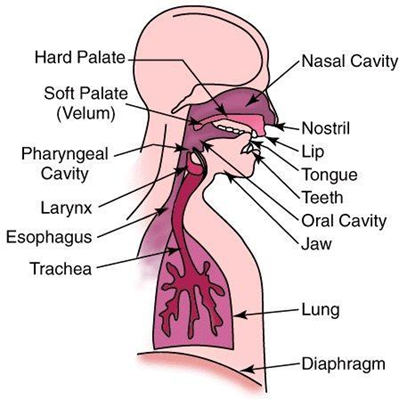
\includegraphics[width=0.8\textwidth]
	{images/chapter2/human-speech-prod}
	\caption{human speech production system.}
	\label{fig:human-speech-prod}
\end{figure}

The speech process starts when air is expelled from the lungs by muscular force providing the source of energy (excitation signal). Then the airflow is modulated in various ways to produce different speech sounds. The modulation is mainly performed in the vocal tract (the main resonant structure), through movements of several articulators, such as the velum, teeth, lips, and tongue. The movements of the articulators modify the shape of the vocal tract, which creates different speech sounds.

\subsubsection{II. Source-Filter Theory of Speech Production}

This model of sound production assumes a source of sound and a filter that shapes that sound, organized so that the source and the filter are independent. This independence allows us to measure and quantify the source separately from the filter (this model also used in LPC analysis discussed in chapter 3).The lungs provide a stream of air, here modelled as the power supply (shown in figure \ref{fig:simple-model-voice-gen}). This stream is then modulated via the vocal folds into three different wave forms:
\begin{itemize}
\item Periodic puffs are responsible for periodic sounds as in $/a/$ or $/o/$. This is generated by the closing of the vocal folds, which then leads to an increase in pressure resulting in a forced opening of the folds and thus again to a decrease in pressure. The vocal folds can close again and the cycle is repeated periodically.
\item Noise occurs when the air stream is directed over halve closed vocal folds. This generates the fricative sounds as in $/f/$ or $/s/$.
\item An impulse is generated similarly to the periodic puffs, but will only involve a single period of the cycle. This leads to the plosive sounds $/p/$, $/t/$, etc.
\end{itemize}

\begin{figure}[ht]
	\centering
	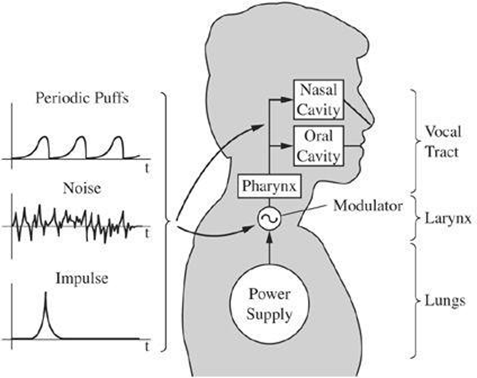
\includegraphics[width=0.8\textwidth]
	{images/chapter2/simple-model-voice-gen}
	\caption{simplified model of voice generation in human body.}
	\label{fig:simple-model-voice-gen}
\end{figure}

This source signal will then propagate through the vocal tract which consists of the throat, the nasal and the oral cavity. This tract will act as a sort of filter that changes and distorts the source, seen in figure \ref{fig:discrete-speech-model}. This happens mainly through resonance and reflections and depends on the shape of the vocal tract. During speaking this shape will change continuously which thus changes the behaviour of the filter.

\begin{figure}[ht]
	\centering
	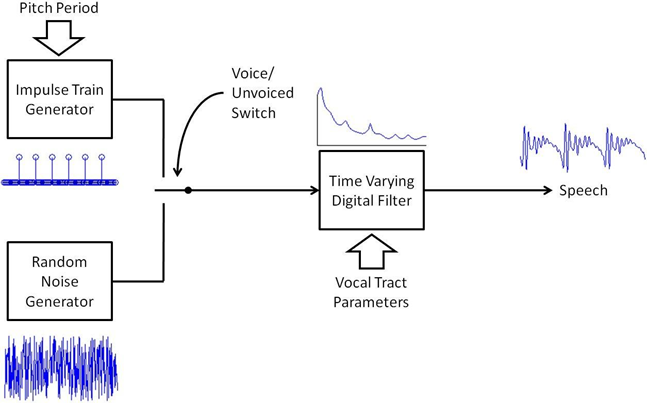
\includegraphics[width=0.8\textwidth]
	{images/chapter2/discrete-speech-model}
	\caption{discrete-time speech production model.}
	\label{fig:discrete-speech-model}
\end{figure}

\subsubsection{III. Fundamental Frequency}
The fundamental frequency, often referred to simply as the fundamental, is defined as the lowest frequency of a periodic waveform (figure \ref{fig:fund-freq-speech}).

\begin{figure}[ht]
	\centering
	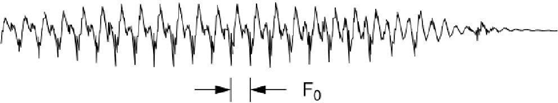
\includegraphics[width=0.8\textwidth]
	{images/chapter2/fund-freq-speech}
	\caption{fundamental frequency of speech signal.}
	\label{fig:fund-freq-speech}
\end{figure}

The fundamental frequency is a measure of how high or low the frequency of a person's voice sounds. Its psychological correlate is pitch. It is the frequency of vocal fold vibration and correlates with changes in vocal fold tension.
\par
A typical adult male will have a fundamental frequency of from 85 to 155Hz, and that of a typical adult female from 165 to 255Hz. Children and babies have even higher fundamental frequencies. Infants show a range of 250 to 650Hz, and in some cases go over 1000Hz. A 10-year-old boy or girl might have a fundamental frequency around 400Hz.

\subsubsection{IV. Formant Frequencies}
The term formant refers to peaks in the harmonic spectrum of a complex sound. Because of their resonant origin, they tend to stay essentially the same when the frequency of the fundamental is changed. There are several formants, each at a different frequency, roughly one in each 1000Hz band. Or, to put it differently, formants occur at roughly 1000Hz intervals. Each formant corresponds to a resonance in the vocal tract (figure \ref{fig:vocal-tract-vowel}).

\begin{figure}[ht]
	\centering
	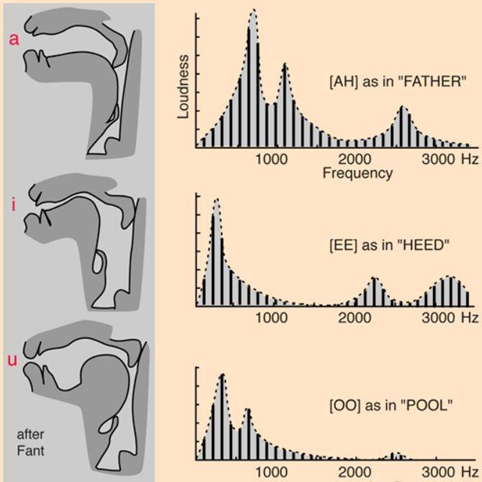
\includegraphics[width=0.8\textwidth]
	{images/chapter2/vocal-tract-vowel}
	\caption{Vocal tract configurations of three different vowels.}
	\label{fig:vocal-tract-vowel}
\end{figure}

Formants are particularly important because they are essential components in the intelligibility of speech. For example, the distinguish-ability of the vowel sounds can be attributed to the differences in their first three formant frequencies. Producing different vowel sounds amounts to retuning these formants within a general range of frequencies.

\begin{figure}[ht]
	\centering
	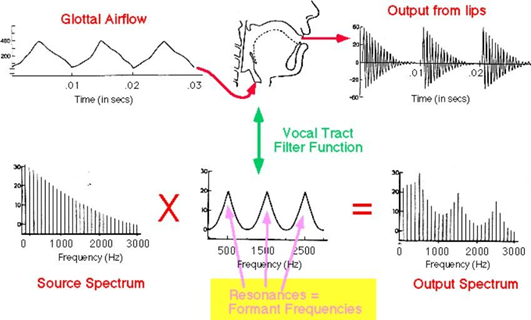
\includegraphics[width=0.8\textwidth]
	{images/chapter2/formant-time-freq}
	\caption{Formants shaping speech in time and frequency domains.}
	\label{fig:formant-time-freq}
\end{figure}

\subsection{Representing Speech in Time and Frequency Domains}
The speech signal is a slowly time varying signal in the sense that, when examined over a sufficiently short period of time (between 5 and 100ms), its characteristics are fairly stationary; however, over long periods of time (on the order of 1/5 seconds or more) the signal characteristics change to reflect the different speech sounds being spoken. There are several ways of classifying (labelling) events in speech. Perhaps the simplest and most straightforward is via the state of the source of speech production-the vocal cords.
\par 
There are several ways of classifying (labelling) events in speech. Perhaps the simplest and most straightforward is via the state of the source of speech production-the vocal cords. It is an accepted convention to use a three-state representation in which the states are:
\begin{itemize}
\item Silence (S):  where no speech is produced.
\item Unvoiced (U): in which the vocal cords are not vibrating, so the resulting speech waveform is aperiodic or random in nature.
\item Voiced (V): in which the vocal cords are tensed and therefore vibrate periodically when air flows from the lungs, so the resulting speech waveform is quasi-periodic.
\end{itemize}
The result of applying this type of classification to a speech signal is shown in Figure \ref{fig:wave-utterance-speech}.

\begin{figure}[ht]
	\centering
	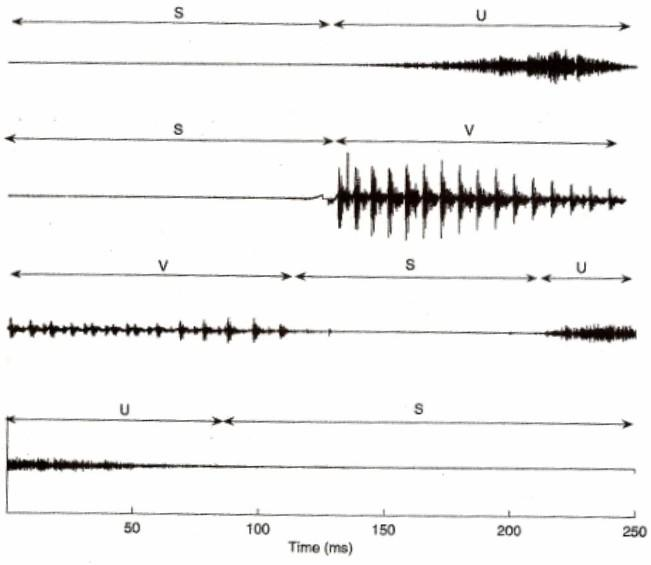
\includegraphics[width=0.8\textwidth]
	{images/chapter2/wave-utterance-speech}
	\caption{Waveform of the utterance ``speech''.}
	\label{fig:wave-utterance-speech}
\end{figure}


An alternative way of characterizing the speech signal and representing the information associated with the sounds is via a spectral representation. Perhaps the most popular representation of this type is the sound spectrogram (Figure \ref{fig:freq-three-formants}) in which a three-dimensional representation of the speech intensity, in different frequency bands on the y-axis, over time represented on the x-axis. Intensity is depicted by the relative darkness of the frequencies shown. The formants (resonant frequencies; the loudest) are the darker bands that correspond to the peaks in the spectrogram.

\subsection{Speech Sounds and Features}
Despite the inherent variance in producing speech sounds, linguists categorize speech sounds (or phones) in a language into units that are linguistically distinct, known as phonemes. There are about 45 phonemes in English. The sounds of a language (phonemes and phonetic variations) are represented by symbols from an alphabet. The most known and long-standing alphabet is the International Phonetic Alphabet (\acrshort{ipa}).
\par
The set of phonemes can be classified into vowels and consonants. Consonant sound is one in which the air flow is cut off, either partially or completely, when the sound is produced. Vowel sound is one in which the air flow is unobstructed when the sound is made.
\subsubsection{I. Vowels}
The vowel sounds are perhaps the most interesting class of sounds in English. Their importance to the classification and representation of written text is very low; however, most practical speech-recognition systems rely heavily on vowel recognition to achieve high performance. Vowels are produced by exciting an essentially fixed vocal tract shape with quasi-periodic pulses of air caused by the vibration of the vocal cords.
\par
The vowels are generally long in duration (as compared to consonant sounds) and are spectrally well defined. As such they are usually easily and reliably recognized and therefore contribute significantly to our ability to recognize speech, both by human beings and by machine.

\begin{figure}[ht]
	\centering
	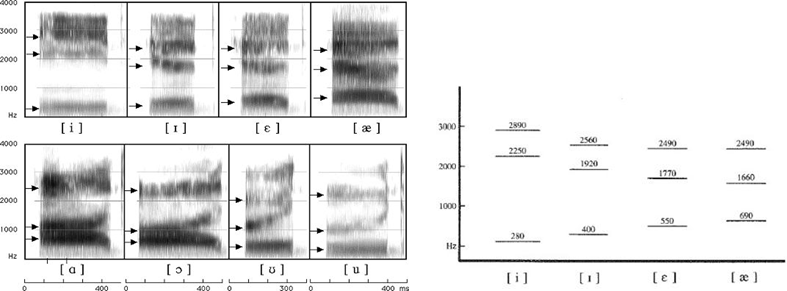
\includegraphics[width=0.8\textwidth]
	{images/chapter2/freq-three-formants}
	\caption{Frequency of the first three formants in eight American English vowels.}
	\label{fig:freq-three-formants}
\end{figure}

\subsubsection{II. Semi-vowels}
The group of sounds consisting of $/w/$, $/l/$, $/r/$, and $/y/$ is quite difficult to characterize. These sounds are called semi-vowels because of their vowel-like nature. They are generally characterized by a gliding transition in vocal tract area function between adjacent phonemes. Thus the acoustic characteristics of these sounds are strongly influenced by the context in which they occur. For our purposes, they are best described as transitional, vowel-like sounds.
\subsubsection{III. Consonants}
Consonants are characterized by momentary interruption or obstruction of the air-stream through the vocal tract. Consonant could have classified by the manner of articulation into five major categories:
\begin{itemize}
\item \textbf{Plosives} \par
Plosive (or oral stop): a complete obstruction of the oral cavity (no air flow) followed by a release of air. Examples of BP phonemes include $/p t k/$ (unvoiced) and $/b d g/$ (voiced). In the voiced consonants, the voicing is the only sound made during the obstruction.
\item \textbf{Fricatives} \par
The air stream is partially obstructed by the close approximation of two articulators at the place of articulation creating a narrow stream of turbulent air. Examples of BP phonemes include $/f/$, $/T/$, $/s/$, $/S/$ (unvoiced) and $/v/$, $/D/$, $/z/$, $/Z/$ (voiced). Voiced fricatives show aspects of both regular vocal fold vibrations and a randomly turbulent air stream. Different from their voiceless counterparts, the voiced fricatives have a substantial voicing bar occupying approximately the lower 400 Hz
\item \textbf{Affricates} \par
An affricate is a consonant that begins as a plosive and releases as a fricative, generally with the same place of articulation. In English, there are just two. One is commonly spelt $[ch]$ and occurs, for instance, in words like chip or church; its IPA symbol is $/tS/$ representing the sequence of plosive $/ t /$ and fricative $/ S /$. The other affricate occurs at the beginning of the word gem or judge and is commonly spelt with $[g]$ or $[j]$, $[dge]$. Its IPA symbol is $/dZ/$ (a voiced combination of $/ d /$ for the plosive element and $/ Z /$ for the fricative element). The bulk of the turbulence of both $/tS/$ and $/dZ/$ occurs above 2000Hz.
\item \textbf{Nasals} \par
It also begins with a complete obstruction of the oral cavity, but with the velum open so that air passes freely through the nasal cavity. The shape and position of the tongue determine the resonant cavity that gives different nasal stops their characteristic sounds. Examples of BP phonemes include $/m n N/$, all voiced.
\end{itemize}

\section{Pre-processing Concept}
The human voice is recorded and digitized. Then it is input to the pre-processing stage. The main task of this stage is to separate out the unvoiced speech samples from the voiced speech samples. The detection of voiced and unvoiced speech can be done on the basis of calculating energy and zero crossing rates frame by frame basis.

\begin{figure}[ht]
	\centering
	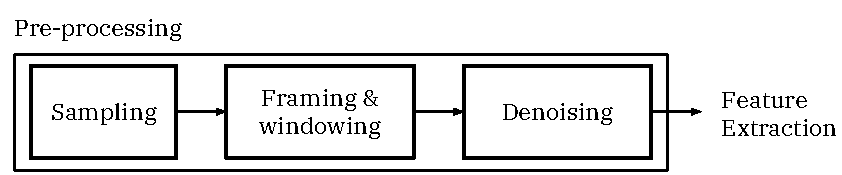
\includegraphics[width=1\textwidth]
	{images/chapter2/general-pre-steps}
	\caption{General steps of the preprocessing stage.}
	\label{fig:general-pre-steps}
\end{figure}

In order that a computer is able to process the speech signal, it first has to be digitized. Therefore, the time-continuous speech signal is sampled and quantized. The result is a time- and value-discrete signal. According to the Nyquist-Shannon sampling theorem a time-continuous signal that is band limited to a certain finite frequency $F_{max}$ needs to be sampled with a sampling frequency of at least $2F_{max}$. Since human speech has a relatively low bandwidth (mostly between 100Hz and 8KHz) a sampling frequency of 44.1KHz is sufficient for speech recognition tasks.

\subsection{Windowing and frame formation}
Speech is a non-stationary time variant signal, because a signal is considered to be stationary if its frequency or spectral components do not change over time. parameter estimation methods require stationary signals Thus dividing the signal into shorter segments (segments, micro-segments, frames) within which the signal behaves (we hope) as stationary.
\par
In order to obtain frames, we multiply the speech signal with a windowing function.

\begin{equation*}
X(f) = S(f) W(f)
\end{equation*}

\subsection{Frame Length}
Frame length must be short enough to assume the signal (within the given length) is stationary, but long enough to provide accurate estimation of the desired parameters (features).

\subsection{Number of frames per segment of the length N}

• In case of No overlap, pram = 0

\begin{figure}[ht]
	\centering
	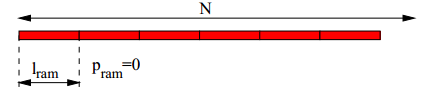
\includegraphics[width=1\textwidth]
	{images/chapter2/frame-wo-overlap}
	\caption{Framing without overlapping.}
	\label{fig:frame-wo-overlap}
\end{figure}

\begin{equation*}
N_{ram} = \left \lfloor \frac{N}{l_{ram}} \right \rfloor
\end{equation*}

• In case of overlap, pram ≠ 0

\begin{figure}[ht]
	\centering
	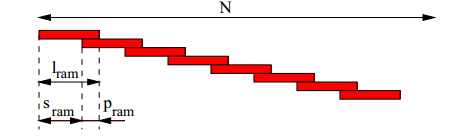
\includegraphics[width=1\textwidth]
	{images/chapter2/frame-overlap}
	\caption{Framing with overlapping.}
	\label{fig:frame-overlap}
\end{figure}

\begin{equation*}
N_{ram} = \left \lfloor \frac{N}{l_{ram}} \right \rfloor
\end{equation*}

\subsection{Select a frame of a signal using a window - windowing function}
\begin{itemize}
\item Rectangular: no change of the signal, selection only.
\begin{equation*}
w(n) =
\begin{cases}
1, & 0 \leq n \leq l_{rem} -1 \\
0, & \text{otherwise}
\end{cases}
\end{equation*}
\item Hamming: suppresses the signal at the sides of the window, selection and weighting.
\begin{equation*}
w(n) =
\begin{cases}
0.54 - 0.46 \cos \frac{2 \pi n}{l_{rem} - 1}, & 0 \leq n \leq l_{rem} -1 \\
0, & \text{otherwise}
\end{cases}
\end{equation*}
\end{itemize}

\subsection{Comparison of rectangular and Hamming windows}
we prefer Hamming window because it doesn't have side loops and in the time domain, the Hamming window does not get as close to zero near the edges.

\begin{figure}[ht]
    \centering
    \begin{subfigure}[b]{1\textwidth}
        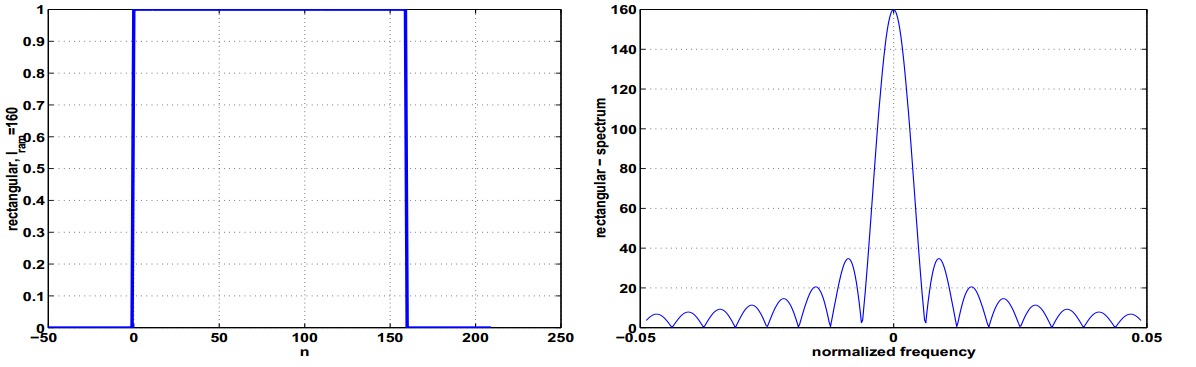
\includegraphics[width=\textwidth]
        {images/chapter2/rect-freq-time}
        \caption{Rectangular}
        \label{fig:rect-freq-time}
    \end{subfigure}

    \begin{subfigure}[b]{1\textwidth}
        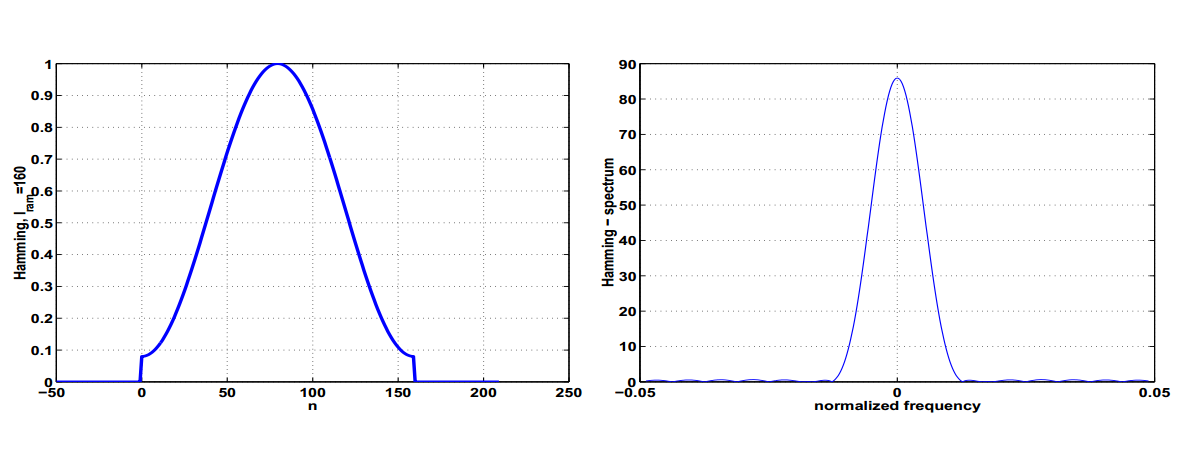
\includegraphics[width=\textwidth]
        {images/chapter2/hamm-freq-time}
        \caption{Hamming}
        \label{fig:hamm-freq-time}
    \end{subfigure}
    \caption{Window in time and frequency domain.}
    \label{fig:window-freq-time}
\end{figure}

\subsection{Denoising \& speech enhancement}
The stage of denoising or noise reduction, also referred to as enhancing of speech degraded by noise, aims to improve the speech signals quality. The objective is to improve the intelligibility, a measure of how comprehensible speech is. Noise corrupting speech signals can be grouped coarsely into the following 3 classes:
\begin{itemize}
\item Microphone related noise.
\item Electrical noise (e.g. electromagnetically induced or radiated noise).
\item Environmental noise.
\end{itemize}

The first two types of noise can be easily compensated by training the speech recognizers on corresponding noisy speech samples, but compensating the environmental noise is not that elementary, due to its high variability. The basic problem of noise reduction is to reduce the external noise without disturbing the unvoiced and low-intensity noise-like components of the speech signal itself.
\par
The algorithms of noise reduction can be grouped into three fundamental classes. In the following exemplary algorithms for denoising are briefly described.
\begin{itemize}
\item Filtering Techniques.
\item Spectral Restoration (speech enhancement).
\item Speech-Model-Based.
\end{itemize}

\begin{figure}[!ht]
	\centering
	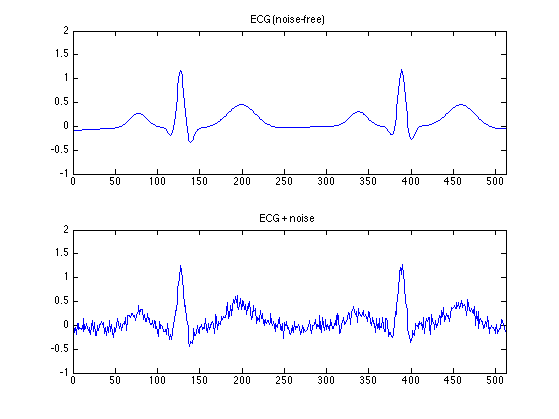
\includegraphics[width=1\textwidth]
	{images/chapter2/signal-noise}
	\caption{Signal without noise and with noise.}
	\label{fig:signal-noise}
\end{figure}

\subsection{Filtering Techniques}
Prominent algorithms based on filtering techniques are Adaptive Wiener filtering and the spectral subtraction methods. Adaptive Wiener filtering depends on the adaptation of (the coefficients of the wiener filter) the filter transfer function from sample to sample based on the speech signal statistics (mean and variance). Spectral subtraction methods estimate the spectrum of the clean signal by the subtraction of the estimated noise magnitude spectrum from the noisy signal magnitude spectrum while keeping the phase spectrum of the noisy signal.

\subsection{Spectral Restoration}
Spectral Restoration refers to the inducing of missing spectral components of non-verbal sounds by adding noise to increase intelligibility. Harmonic Decomposition refers to a denoising technique that uses a harmonic+noise model of the speech, assuming that the speech signal is composed of a periodic/voiced and random/unvoiced part. By processing the components separately and recombining them, the speech signal can be enhanced.

\subsection{voiced and unvoiced speech}
The determination of voiced and unvoiced speech samples can be done on the basis of Energy and Zero crossing rates (\acrshort{zcr}).

\begin{figure}[ht]
	\centering
	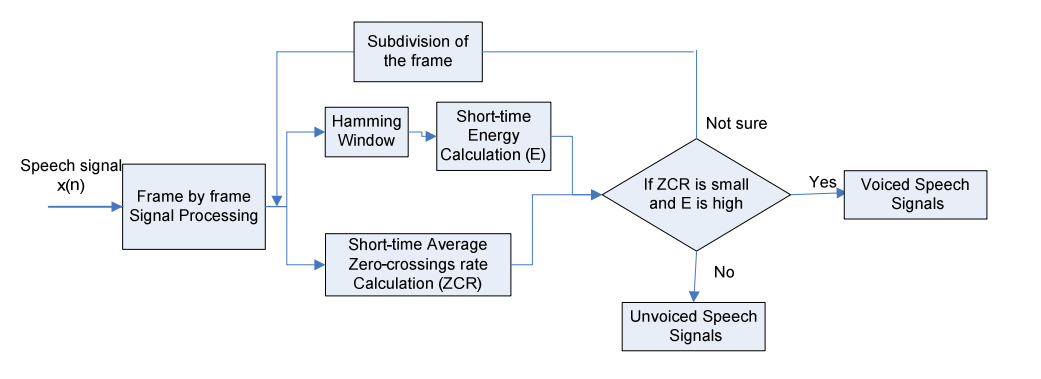
\includegraphics[width=1\textwidth]
	{images/chapter2/algorithm-voiced-unvoiced}
	\caption{Algorithm to determine whether speech is voiced or unvoiced.}
	\label{fig:algorithm-voiced-unvoiced}
\end{figure}

\subsubsection{Average Short-Time Energy}
 The energy of speech is calculated frame by frames. The square of each sample is done and finally summation of all squared samples is done. separation of phonemes to voiced (high energy) and unvoiced (low energy).

\begin{equation*}
E = \frac{1}{l_{ram}} \sum_{n=0}^{l_{ram} - 1} x^2 [n]
\end{equation*}

\subsubsection{Zero Crossing Rate (ZCR)}
The zero crossing rates mean the number of times the transition of speech signal from positive to negative or vice versa. The zero crossing rates are calculated frame by frames. If the ZCR of speech samples having more zero crossing rates then it is an unvoiced otherwise voiced.

\begin{equation*}
E = \frac{1}{2} \sum_{n=1}^{l_{ram} - 1} \left | \, \text{sign} \, x[n] - \text{sign} \, x[n-1] \, \right |
\end{equation*}
where $\text{sign} \, x[n]$ is the sign function defined as

\begin{equation*}
\text{sign} \, x[n] = \begin{cases}
1, & x[n] \geq 0 \\ 
-1, & x[n] < 0
\end{cases}
\end{equation*}

\begin{figure}[ht]
	\centering
	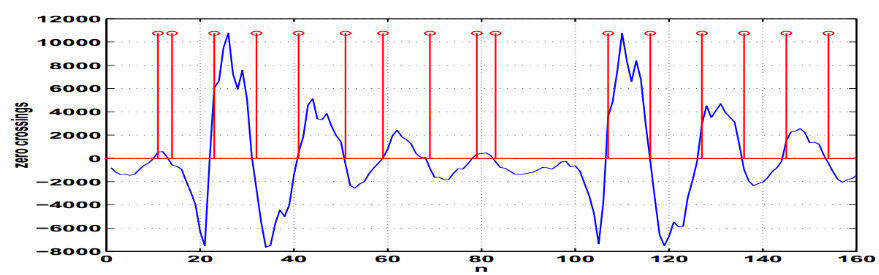
\includegraphics[width=1\textwidth]
	{images/chapter2/low-high-zcr}
	\caption{Distinguishing between the voiced (low zero-crossing rate) and unvoiced (high rate, rather like in noise).}
	\label{fig:low-high-zcr}
\end{figure}

\subsection{Silence Removal} 
Pre-processing of Speech Signal serves various purposes in any speech processing application. It includes Noise Removal, Endpoint Detection, Pre-emphasis, Framing, Windowing, Echo Cancelling etc. Out of these, silence/unvoiced portion removal along with endpoint detection is the fundamental step for applications like Speech and Speaker Recognition. The proposed method uses Probability Density Function (\acrshort{pdf}) of the background noise and a Linear Pattern Classifier for classification of Voiced part of a speech from silence/unvoiced part. The work shows better end point detection as well as silence removal than conventional Zero Crossing Rate (ZCR) and Short Time Energy (\acrshort{ste}) function methods.
\par
It should be clear that the segmentation of the waveform into well-defined regions of silence, unvoiced, signals is not exact; it is often difficult to distinguish a weak, unvoiced sound (like /f/ or /th/) from silence, or weak voiced sound (like /v/ or /m/) from unvoiced sounds or even silence. However, it is usually not critical to segment the signal to a precision much less than several milliseconds; hence, small errors in boundary locations usually have no consequence for most applications. Since for most of the practical cases the unvoiced part has low energy content and thus silence (background noise) and unvoiced part is classified together as silence/unvoiced and is distinguished from voiced part. 
\par
Two widely accepted methods namely Short Time Energy (STE) and Zeros Crossing Rate (ZCR) have been used for a long time for silence removal. But they have their own limitation regarding setting thresholds as an ad-hoc basis. STE uses the fact that energy in voiced sample is greater than silence/unvoiced sample. However, it is not specific about how much greater it needs to be for proper classification and varies case to case. On the other hand ZCR has a demarcation rule specifying that if the ZCR of a portion speech exceeds 50 then this portion will be labelled as unvoiced or background noise whereas any segment showing ZCR at about 12 is considered to be the voiced one. One attempt was made by taking these two methods together and results reported only 65\% accuracy with respect to manually labelled speech sample.
\par
Here, we detect silence/unvoiced part from the speech sample using uni-dimensional Mahalanobis Distance  function which itself is a Linear Pattern Classifier. Our algorithm uses statistical properties of background noise as well as physiological aspect of speech production and does not assume any ad-hoc threshold. We also show the algorithm's performance using the measure of correctness taking manually labelled speech as a reference. The experiments are done on two kinds of speeches which are a running text read from a paragraph and a combination lock number. The result shows better classification for the proposed method in both the cases when compared against conventional silence/unvoiced detection methods. We assume that background noise present in the utterances are Gaussian in nature, however a speech signal may also be contaminated with different types of noise. In such cases the corresponding properties of the noise distribution function are to be used for detection purpose.


\subsubsection{Theory}
\subsubsection{Gaussian or Normal Distribution}
One of the most important results of the probability theory is the Central Limit Theorem, which states that, under various conditions, the distribution for the sum of d independent random variables approaches a particular limiting form known as the normal distribution. As such, the normal or Gaussian probability density function is very important, both for theoretical and practical reasons. In one dimension, it is defined by
\begin{equation*}
p(x) = \frac{1}{\sigma \sqrt{2\pi }} e^{-\frac{1}{2}\left ( \frac{x-\mu }{\sigma } \right )^{2}}
\end{equation*}
The normal density is traditionally described as ``bell-shaped curve''; it is completely determined by the numerical values for two parameters, the mean $\mu$ and the variance $\sigma^2$. This is often emphasized by writing $p(x)~N(\mu,\sigma^2)$, which is read as ``x is distributed normally with mean $\mu$ and variance $\sigma^2$''. The distribution is symmetrical about the mean, the peak occurring at $x=\mu$ and the width of the ``bell'' is proportional to the standard deviation $\sigma$. Normally distributed data points tend to cluster about the mean. Numerically, the probabilities obey
\begin{align}
P[|x-\mu| \leq \sigma] &= 0.68 \nonumber \\ 
P[|x-\mu| \leq 2\sigma] &= 0.95 \nonumber \\ 
P[|x-\mu| \leq 3\sigma] &= 0.997 \label{eq:gaussian-majority}
\end{align}
as shown in figure \ref{fig:gaussian}
\begin{figure}[ht]
	\centering
	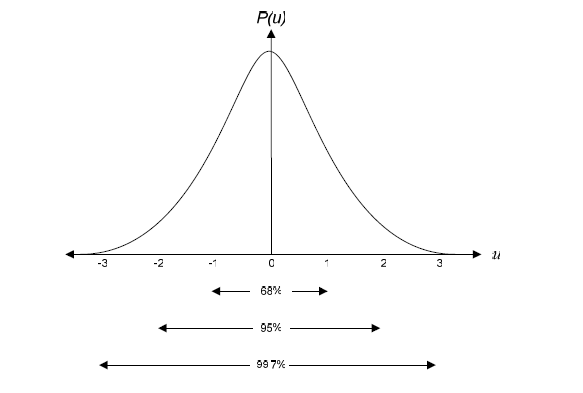
\includegraphics[width=1\textwidth]
	{images/chapter2/gaussian}
	\caption{A one-dimensional Gaussian distribution $P(u)~N(0,1)$, has 68\% of its probability mass in the range $|u|\leq 1$, 95\% in the range of $|u|\leq 2$, and 99.7\% in the range of $|u|\leq 3$.}
	\label{fig:gaussian}
\end{figure}

A natural measure of the distance from x to the mean is the distance $|x - \mu |$ measured in units of standard deviation which can be analytically expressed as

\begin{equation*}
r = \frac{|x - \mu |}{\sigma}
\end{equation*}

and defined as ``Mahalanobis Distance'' from $x$ to $\mu$ (In the one-dimensional case, this is sometimes called z-score). Thus for instance the probability is 0.95 that the Mahalanobis distance from x to μ will be less than 2. If a random variable $x$ is modified by (a) subtracting its mean and (b) dividing by its standard deviation, it is said to be standardized. Clearly, a standardized normal random variable $r$ has zero mean and unit standard deviation-that is,
\begin{equation*}
p(u) = \frac{1}{\sqrt{2\pi }} e^{-\frac{u^2}{2}}
\end{equation*}
which can be written as $P(u)~N(0,1)$.

\subsubsection{Algorithm}
The algorithm described below is divided into two parts. First part assigns label to the samples by using a statistical properties of background noise while the second part smooths the labeling by the physiological aspects from the speech production process. The Algorithm two passes over speech samples. In Pass I (Step 1 to 3) we use statistical property of background noise to make a sample.
\par
use physiological aspects of speech production for smoothing and reduction of probabilistic errors in statistical marking of Pass I.

\subsubsection{Steps}
\begin{enumerate}
\item Calculate the mean and standard deviation of the first 1600 samples of the given utterance. If $\mu$ and $\sigma$ are the mean and the standard deviation respectively then analytically we can write,
\begin{align*}
\mu &= \frac{1}{1600} \sum_{i=1}^{1600} x(i) \\
\mu &= \sqrt{\frac{1}{1600} \sum_{i=1}^{1600} x(i - \mu)^2}
\end{align*}
Note that background noise is characterized by this $\mu$ and $\sigma$.
\item Go from first sample to the last sample of the speech recording. In each sample check whether one-dimensional Mahalanobis distance function greater than 3 or not. Analytically if,
\begin{equation*}
\frac{|x - \mu |}{\sigma} > 3
\end{equation*}
the sample is to be treated as voiced sample otherwise it is an silence/unvoiced. Note that the threshold reject the samples upto 99.7\% as per equation \ref{eq:gaussian-majority} in a Gaussian Distribution thus accepting only the voiced samples.

\item Mark the voiced sample as 1 and unvoiced sample as 0. Divide the whole speech signal into 10ms non-overlapping windows. Now the complete speech is represented by only zeros and ones.

\item Consider there are $M$ no. of zeros and number of ones in a window. If $M \geq N$ then convert each of ones to zeros and vice versa. This method adopted here keeping in mind that a speech production system consisting of vocal chord, tongue, vocal tract etc. cannot change abruptly in a short period of time window taken here as 10ms.

\item Collect the voiced part only according to the labelled ``1'' samples from the windowed array and dump it in a new array. Retrieve the voiced part of the original speech signal from labelled 1 samples, The algorithm is illustrated in the flow chart given in figure \ref{fig:s-remove-algorithm}

\end{enumerate}

Note that in the proposed method after $\mu$ and $\sigma$ calculation it requires one division and condition checking per sample in Pass I and in Pass II one condition checking per 80 samples (10ms). In ZCR method sign of each sample is checked and number of reversal in a window (80 samples, 10 ms) is calculated. Then the no. of sign reversal is checked if within certain range for voice part classification purpose. In STE method each sample sequence energy is calculated and then summed over 80 samples (10ms) window. Then a condition checking is done on this sum to classify it as voiced part or not. Thus the proposed method is computationally comparable to figure \ref{fig:s-remove-algorithm}

\begin{figure}[!h]
	\centering
	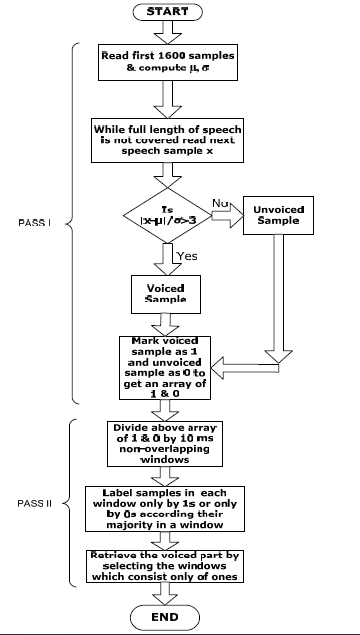
\includegraphics[width=0.6\textwidth]
	{images/chapter2/s-remove-algorithm}
	\caption{Flow Chart of the algorithm.}
	\label{fig:s-remove-algorithm}
\end{figure}

Conventional STE \& ZCR based silence/unvoiced detection method and can be used for real time analysis.


\section*{References}
\begin{enumerate}
\item J.L. Flanagan, Speech Analysis, Synthesis, and Perception, 2nd ed., Springer-Verlag, New York, (1972).
\item Hofmann,Y.H, Speech recognition for human computer Interaction (2009).
\item hyper physics, http://hyperphysics.phy-astr.gsu.edu/hbase/Music/.
\item Rabiner, L.R., Juang, B.H. Fundamentals of Speech Recognition, Prentice-Hall, NJ (1993).
\item Adami, A.G. Automatic Speech Recognition: From the Beginning to the Portuguese Language.
\item J. P. Campbell, Jr., “Speaker Recognition: A Tutorial”, Proceedings of The IEEE, Vol.85, No.9, pp.1437-1462, Sept.1997. 
\item Koji Kitayama, Masataka Goto, Katunobu Itou and Tetsunori Kobayashi, “Speech Starter: Noise-Robust Endpoint Detection by Using Filled Pauses”, Eurospeech 2003, Geneva, pp. 1237-1240. 
\item S. E. Bou-Ghazale and K. Assaleh, “A robust endpoint detection of speech for noisy environments with application to automatic speech recognition”, in Proc. ICASSP2002, vol. 4, 2002, pp. 3808–3811.
\end{enumerate}








































































































































%%%%%%%%%%%%%%%%%%%%%%%%%%%%%%%%%%%%%%%%%%%%%%%%%%%%%%%%%%%%%%%%%%%%%%%%%%%%%%%%%%%%%%%%%%%%%%%%%%%%%%%%%%%%%%%%%%%%%%%%%%%%%%%%%%%%%%%%%%%%%%%%%%%%%%%%%%%%%%%%%%%%%%%%%%%%%%%%%%%%%%%%%%%%%%% CHAPTER 3 %%%%%%%%%%%%%%%%%%%%%%%%%%%%%%%%%%%%%%%%%%%%%%%%%%%%%%%%%%%%%%%%%%%%%%%%%%%%%%%%%%%%%%%%%%%%%%%%%%%%%%%%%%%%%%%%%%%%%%%%%%%%%%%%%%%%%%%%%%%%%%%%%%%%%%%%%%%%%%%%%%%%%%%%%%%%%%%%%%%%%%%%%%%%

\chapter{Feature Extraction}
\section{Mel-Frequency Cepstral Coefficient}
\subsection{Introduction}
Speech recognition system processes the word uttered by the user and extracts its features. When the user utters something, it is sent to the speech engine to be processed then converted into digital domain. The digitalized speech samples are processed to extract features using MFCC and other algorithms. Once the desired number of features is obtained, they can be sent through feature matching stage.
\par
The main purpose of the MFCC processor is to mimic the behavior of the human ears. The sounds generated by a human are filtered by the shape of the vocal tract including tongue, teeth etc. This shape determines what sound comes out. If we can determine the shape accurately, this should give us an accurate representation of the phoneme being produced. The shape of the vocal tract manifests itself in the envelope of the short time power spectrum, and the job of MFCCs is to accurately represent this envelope.
\begin{figure}[!h]
	\centering
	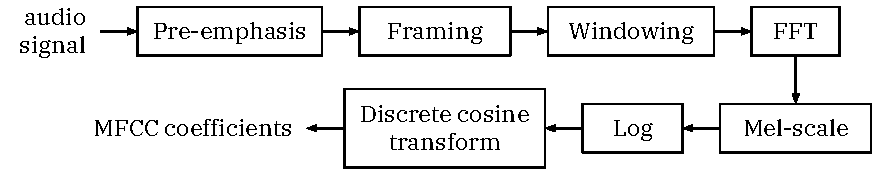
\includegraphics[width=0.8\textwidth]
	{images/chapter3/mfcc}
	\caption{MFCC Block Diagram.}
	\label{fig:mfcc}
\end{figure}

\subsection{Pre-emphasis}
The first stage in MFCC feature extraction is to boost the amount of energy in the high frequencies. It turns out that if we look at the spectrum for voiced segments like vowels, there is more energy at the lower frequencies than the higher frequencies. This drop in energy across frequencies (which is called spectral tilt) is caused by the nature of the glottal pulse. Boosting the high frequency energy makes information from these higher formants more available to the acoustic model and improves phone detection accuracy.This pre-emphasis is done by using a filter. figure \ref{fig:pre-emphasis} shows an example of a spectral of the single vowel [aa] before and after pre-emphasis.

\begin{figure}[!h]
	\centering
	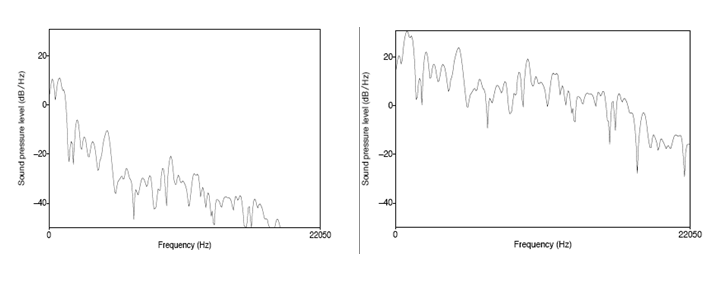
\includegraphics[width=0.8\textwidth]
	{images/chapter3/pre-emphasis}
	\caption{example of a spectral slice of the single vowel [aa]  a)before,  b) after pre-emphasis.}
	\label{fig:pre-emphasis}
\end{figure}

\subsection{Framing and Blocking}
In this step the continuous 1D signal are blocked into small frames of $N$ samples, with next frames separated by $M$ samples (M<N) with this the adjacent frames are overlapped by $N-M$ samples. As per many researches the standard value taken for $N=256$ and $M=100$ with a reason of dividing the given 1D  signal  into  small  frames  having  sufficient  samples  to  get  enough  information.  Because, if the frame size smaller than this size is taken then the number of samples in the frames will not be enough  to  get  the  reliable  information  and  with  large  size  frames  it  can  cause  frequent  change  in  the  information  inside  the  frame.  So, while   working with MFCC  these  parameters  are  very  common  in  practice. This process of breaking up the signals into frames will continue until the whole 1D signal is broken down into small frames.

\subsection{Windowing}
Windowing   is done for  minimizing  the  disruptions  at  the  starting  and  at  the  end  of  the  frame, the frame and window function is being multiplied. If the window being defined is $W_n(m)$, $0 \leq m \leq N_{m-1}$ where $N_m$ stands for the quantity of samples within every frame, the output after windowing the signal will be presented as $Y(m) = X(m)W_n(m), 0 ≤ m ≤ N_{m-1}$ where $Y(m)$ represents the output signal after multiplying the input signal represented as $X(m)$ and Hamming window represented by $W_n(m)$. Figure \ref{fig:hamming} illustrates the  effect of the hamming window on the speech signal.
\begin{figure}[!h]
	\centering
	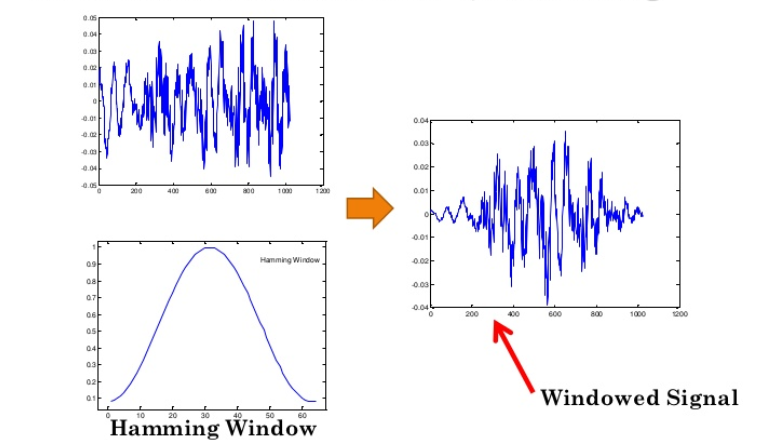
\includegraphics[width=1\textwidth]
	{images/chapter3/hamming}
	\caption{example of a spectral slice of the single vowel [aa]  a)before,  b) after pre-emphasis.}
	\label{fig:hamming}
\end{figure}

Basically,  many  window  functions  exist  such  as  rectangular  window,  flat  top  window  and  hamming window  but,  mainly  hamming  window  is  applied  for  carrying  out  windowing  which  usually represented as:
\begin{equation*}
W_n(m) = 0.54 - 0.46\cos \left ( \frac{2\pi m}{N_m -1} \right ), \; \; 0 \leq m\leq N_m -1
\end{equation*}

\subsection{Fast Fourier Transform}
FFT is used for doing conversion from the spatial domain to the frequency domain. Each frame having $N_m$ samples are converted into frequency domain. Fourier transformation is a fast algorithm to apply Discrete Fourier Transform (DFT), on the given set of $N_m$ samples shown below:
\begin{equation*}
D_k = \sum_{m=0}^{N_m -1}D_m e^{-2j\pi k\frac{m}{N_m}}, \; k=0,1,2,...,N_m - 1
\end{equation*}
Basically the definition for FFT and DFT is same, which means that the output for the transformation will be the same; however they differ in their computational complexity. In case of DFT, each frame with $N-M$ samples directly will be used as a sequence for Fourier transformation. On another, in case of FFT this frame will be divided into small DFT’s and then computation will be done on this divided small   DFT’s  as  individual  sequence  thus  the  computation  will  be  more  fast  and  easy.  Thus  it  is  in digital processing or other area instead of directly using DFT, FFT is used for applying DFT.

\subsection{Mel-scale}
The human cochlea (an organ in the ear) vibrates at different spots depending on the frequency of the incoming sounds. Depending on the location in the cochlea that vibrates (which wobbles small hairs), different nerves fire informing the brain that certain frequencies are present.
\par
In particular the cochlea can't discern the difference between two closely spaced frequencies. This effect becomes more pronounced as the frequencies increase. For this reason, we take clumps of periodogram bins and sum them up to get an idea of how much energy exists in various frequency regions. This is performed by our Mel filter bank: the first filter is very narrow and gives an indication of how much energy exists near 0 Hertz. As the frequencies get higher our filters get wider as we become less concerned about variations. We are only interested in roughly how much energy occurs at each spot. The Mel scale tells us exactly how to space our filter banks and how wide to make them.
\par
So, The Mel scale relates perceived frequency, or pitch, of a pure tone to its actual measured frequency. Humans are much better at discerning small changes in pitch at low frequencies than they are at high frequencies. Incorporating this scale makes our features match more closely what humans hear.
\par
The formula to convert frequency $f$ hertz into Mel $m_f$ is,  
\begin{equation*}
m_f = 2595\log \left ( \frac{f}{100} + 1 \right )
\end{equation*}
During the mapping, when a given frequency value is up to 1000Hz  the  Mel-frequency  scaling  is  linear  frequency  spacing,  but  after  1000Hz  the  spacing  is logarithmic as shown in figure \ref{fig:mel-scale}.
\begin{figure}[!h]
	\centering
	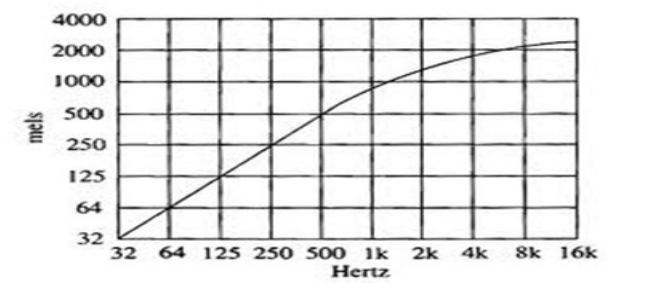
\includegraphics[width=0.7\textwidth]
	{images/chapter3/mel-scale}
	\caption{relation between mel-scale and linear  frequency scale.}
	\label{fig:mel-scale}
\end{figure}

\begin{figure}[!h]
	\centering
	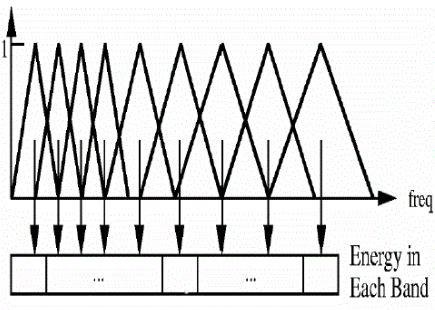
\includegraphics[width=0.7\textwidth]
	{images/chapter3/mel-banks}
	\caption{filter banks(same width until 1KHZ after 1K as the frequency increases the width get wider).}
	\label{fig:mel-banks}
\end{figure}

\subsection{Log}
Once we have the filter bank energies, we take the logarithm of them. This is also motivated by human hearing: we don't hear loudness on a linear scale. Generally, to double the perceived volume of a sound we need to put 8 times as much energy into it. This means that large variations in energy may not sound all that different if the sound is loud to begin with. This compression operation makes our features match more closely what humans actually hear. Why the logarithm and not a cube root? The logarithm allows us to use cepstral mean subtraction, which is a channel normalization technique.

\subsection{Discrete cosine Transform (DCT)}
This process of carrying  out  DCT  is  done  in  order  to  convert  the  log  Mel  spectrum  back  into  the spatial  domain.  For this transformation either  DFT  or  DCT  both  can  be  used  for  calculating Coefficients from the given log Mel spectrum as they divide a given sequence of finite length data into discrete  vector.  However,  DFT  is  generally  used  for  spectral  analysis  where  as  DCT  used  for  data compression  as  DCT  signals  have  more  information  concentrated  in  a  small  number  of  coefficients and hence, it is easy and requires less storage to represent Mel spectrum in a relative small number of coefficients.  This instead of  using  DFT  DCT  is  desirable  for  the coefficients calculation  as  DCT outputs can contain important amounts of energy. The output after applying DCT is known as MFCC (Mel Frequency Cepstrum Coefficient)

\begin{equation*}
C_n = \sum_{k-1}^{k}\left ( \log D_k \right )\cos \left [ m(k-0.5) \left ( \frac{\pi}{k} \right ) \right ], \; m=0,1,...,k-1
\end{equation*}

where $C_n$ represents the MFCC and $m$ is the number of the coefficients.

\section{Discrete Wavelet Transform}
\subsection{Introduction}
In 19th century, the French mathematician J. Fourier, showed that any periodic function can be expressed as an infinite sum of periodic complex exponential functions. Many years after he had discovered this remarkable property of (periodic) functions, his ideas were generalized to first non-periodic functions, and then periodic or non-periodic discrete time signals. It is after this generalization that it became a very suitable tool for computer calculations. In 1965, a new algorithm called Fast Fourier Transform (FFT) was developed and FT became even more popular.
\par
FT decomposes a signal to complex exponential functions of different frequencies. The way it does this, is defined by the following two equations:
\begin{align}
X(f) &= \int_{-\infty}^{\infty} x(t) . e^{-2j\pi ft} \, \text{d}t \label{eq:fourier-transform} \\
x(t) &= \int_{-\infty}^{\infty} X(f) . e^{2j\pi ft} \, \text{d}f \nonumber
\end{align}

In the above equation, $t$ stands for time, $f$ stands for frequency, and x denotes the signal at hand. Note that $x$ denotes the signal in time domain and the $X$ denotes the signal in frequency domain. This convention is used to distinguish the two representations of the signal. The first Equation is called the Fourier transform of $x(t)$, and the second equation is called the inverse Fourier transform of $X(f)$, which is $x(t)$.
\par
The signal $x(t)$, is multiplied with an exponential term, at some certain frequency $f$, and then integrated over time.

\begin{figure}[!h]
    \centering
    \begin{subfigure}[b]{0.7\textwidth}
        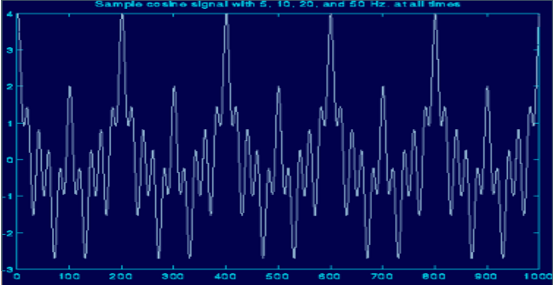
\includegraphics[width=\textwidth]
        {images/chapter3/ft-signal-time}
        \caption{time domain}
        \label{fig:ft-signal-time}
    \end{subfigure}

    \begin{subfigure}[b]{0.7\textwidth}
        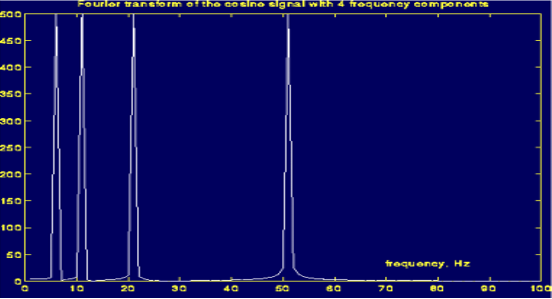
\includegraphics[width=\textwidth]
        {images/chapter3/ft-signal-freq}
        \caption{frequency domain}
        \label{fig:ft-signal-freq}
    \end{subfigure}
    \caption{representation of equation \ref{eq:ft-signal}.}
    \label{fig:ft-signal}
\end{figure}

IMPORTANT: The information provided by the integral, corresponds to all time instances, since the integration is from minus infinity to plus infinity over time. It follows that no matter where in time the component with frequency $f$ appears, it will affect the result of the integration equally as well. In other words, whether the frequency component $f$ appears at time $t_1$ or $t_2$, it will have the same effect on the integration. This is why Fourier transform is not suitable if the signal has time varying frequency, i.e., the signal is non-stationary. If only, the signal has the frequency component $f$ at all times (for all $f$ values), then the result obtained by the Fourier transform makes sense.
\par
Note that the Fourier transform tells whether a certain frequency component exists or not. This information is independent of where in time this component appears. It is therefore very important to know whether a signal is stationary or not, prior to processing it with the FT.
\par
Look at figure \ref{fig:ft-signal}, which shows the signal,
\begin{equation}
x(t) = \cos(2\pi 5t) + \cos(2\pi 10t) + \cos(2\pi 20t) + \cos(2\pi 50t)
\label{eq:ft-signal}
\end{equation}
that is, it has four frequency components of 5, 10, 20, and 50 Hz, all occurring at all times.
\subsection{Short-term Fourier Transform}
Note the four peaks in the above figure, which correspond to four different frequencies. Now, look at the following figure: Here the signal is again the cosine signal, and it has the same four frequencies. However, these components occur at different times.
\begin{figure}[H]
    \centering
    \begin{subfigure}[b]{0.7\textwidth}
        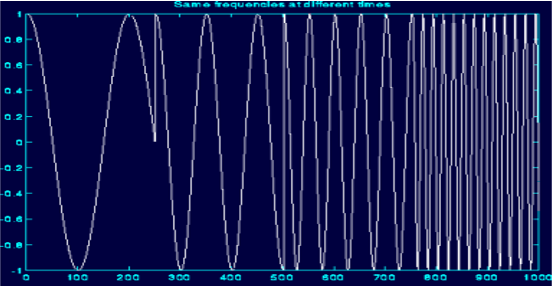
\includegraphics[width=\textwidth]
        {images/chapter3/ft-fail-signal-time}
        \caption{time domain}
        \label{fig:ft-fail-signal-time}
    \end{subfigure}

    \begin{subfigure}[b]{0.7\textwidth}
        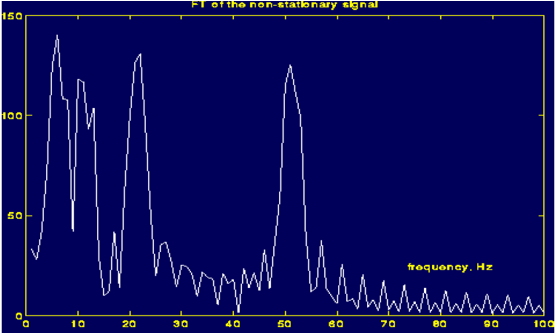
\includegraphics[width=\textwidth]
        {images/chapter3/ft-fail-signal-freq}
        \caption{frequency domain}
        \label{fig:ft-fail-signal-freq}
    \end{subfigure}
    \caption{}
    \label{fig:ft-fail-signal}
\end{figure}
What you are supposed to see in the above figure, is it is (almost) same with the previous FT figure. Please look carefully and note the major four peaks corresponding to 5, 10, 20, and 50 Hz. As you can see from the above example, FT cannot distinguish the two signals very well. To FT, both signals are the same, because they constitute of the same frequency components. Therefore, FT is not a suitable tool for analyzing non-stationary signals, i.e., signals with time varying spectra.
\par
So, how are we going to insert this time business into our frequency plots? Let's look at the problem in hand little closer. 
What was wrong with FT? It did not work for non-stationary signals. Let's think this: Can we assume that, some portion of a non-stationary signal is stationary? 
The answer is yes. 
Just look at the third figure above. The signal is stationary every 250 time unit intervals. 
You may ask the following question? 
What if the part that we can consider to be stationary is very small? 
Well, if it is too small, it is too small. There is nothing we can do about that, and actually, there is nothing wrong with that either. We have to play this game with the physicists' rules. 
If this region where the signal can be assumed to be stationary is too small, then we look at that signal from narrow windows, narrow enough that the portion of the signal seen from these windows are indeed stationary. 
This approach of researchers ended up with a revised version of the Fourier transform, so-called: The Short Time Fourier Transform (STFT).
There is only a minor difference between STFT and FT. In STFT, the signal is divided into small enough segments, where these segments (portions) of the signal can be assumed to be stationary. For this purpose, a window function "w" is chosen. The width of this window must be equal to the segment of the signal where its stationarity is valid.
This window function is first located to the very beginning of the signal. That is, the window function is located at t=0. Let's suppose that the width of the window is "T" s. At this time instant (t=0), the window function will overlap with the first T/2 seconds (I will assume that all time units are in seconds). The window function and the signal are then multiplied. By doing this, only the first T/2 seconds of the signal is being chosen, with the appropriate weighting of the window (if the window is a rectangle, with amplitude "1", then the product will be equal to the signal). Then this product is assumed to be just another signal, whose FT is to be taken. In other words, FT of this product is taken, just as taking the FT of any signal. 
The result of this transformation is the FT of the first T/2 seconds of the signal. If this portion of the signal is stationary, as it is assumed, then there will be no problem and the obtained result will be a true frequency representation of the first T/2 seconds of the signal. 
The next step, would be shifting this window (for some t1 seconds) to a new location, multiplying with the signal, and taking the FT of the product. This procedure is followed, until the end of the signal is reached by shifting the window with "t1" seconds intervals.
\begin{equation*}
STFT^{(\omega)}_{X}(t, f) = \int_{t}\left [ x(t) . \omega^{*}(t-t')  \right ] e^{-2j\pi ft} \text{d}t
\end{equation*}
x(t) is the signal itself, w(t) is the window function.
\par
The problem with the STFT has something to do with the width of the window function that is used. To be technically correct, this width of the window function is known as the support of the window. If the window function is narrow, than it is known as compactly supported. This terminology is more often used in the wavelet world, as we will see later.

\subsection{Continuous Wavelet Transform}
The continuous wavelet transform was developed as an alternative approach to the short time Fourier transform to overcome the resolution problem. The wavelet analysis is done in a similar way to the STFT analysis, in the sense that the signal is multiplied with a function, {\it the wavelet}, similar to the window function in the STFT, and the transform is computed separately for different segments of the time-domain signal. However, there are two main differences between the STFT and the CWT: 
\begin{enumerate}
\item The Fourier transforms of the windowed signals are not taken, and therefore single peak will be seen corresponding to a sinusoid, i.e., negative frequencies are not computed. 
\item The width of the window is changed as the transform is computed for every single spectral component, which is probably the most significant characteristic of the wavelet transform. 
\end{enumerate}
The continuous wavelet transform is defined as follows
\begin{align*}
CWT_{x}^{\psi}(\tau, s) = \Psi (\tau, s) &= \frac{1}{\sqrt{\left | s \right |}} \int x(t) \psi^{*} \left ( \frac{t-\tau}{s} \right ) \text{d}t \\
\psi_{t,s} &= \frac{1}{\sqrt{s}} \psi \left ( \frac{t - \tau}{s} \right )
\end{align*}
As seen in the above equation, the transformed signal is a function of two variables, tau and s, the translation and scale parameters, respectively. $\psi(t)$ is the transforming function, and it is called the mother wavelet. The term mother wavelet gets its name due to two important properties of the wavelet analysis as explained below.
\par
The term wavelet means a small wave. The smallness refers to the condition that this (window) function is of finite length (compactly supported). The wave refers to the condition that this function is oscillatory. The term mother implies that the functions with different region of support that are used in the transformation process are derived from one main function, or the mother wavelet. In other words, the mother wavelet is a prototype for generating the other window functions. 
\par
The term translation is used in the same sense as it was used in the STFT; it is related to the location of the window, as the window is shifted through the signal. This term, obviously, corresponds to time information in the transform domain. However, we do not have a frequency parameter, as we had before for the STFT. Instead, we have scale parameter which is defined as 1/frequency. The term frequency is reserved for the STFT. Scale is described in more detail in the next section.
\subsubsection{The Scale}
The parameter scale in the wavelet analysis is similar to the scale used in maps. As in the case of maps, high scales correspond to a non-detailed global view (of the signal), and low scales correspond to a detailed view. Similarly, in terms of frequency, low frequencies (high scales) correspond to a global information of a signal (that usually spans the entire signal), whereas high frequencies (low scales) correspond to a detailed information of a hidden pattern in the signal (that usually lasts a relatively short time). Cosine signals corresponding to various scales are given as examples in figure \ref{fig:cwt-scale}.

\begin{figure}[!h]
	\centering
	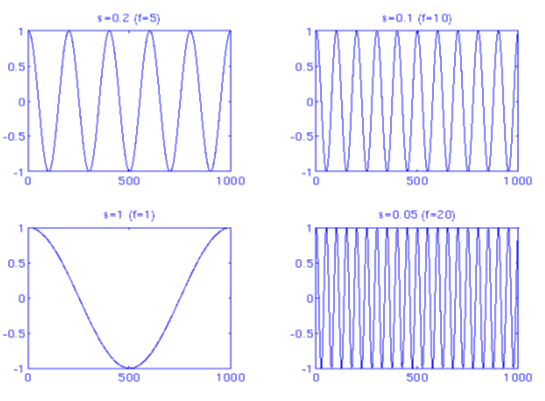
\includegraphics[width=0.6\textwidth]
	{images/chapter3/cwt-scale}
	\caption{}
	\label{fig:cwt-scale}
\end{figure}

Fortunately, in practical applications, low scales (high frequencies) do not last for the entire duration of the signal, unlike those shown in the figure, but they usually appear from time to time as short bursts, or spikes. High scales (low frequencies) usually last for the entire duration of the signal.
\par
Scaling, as a mathematical operation, either dilates or compresses a signal. Larger scales correspond to dilated (or stretched out) signals and small scales correspond to compressed signals. All of the signals given in the figure are derived from the same cosine signal, i.e., they are dilated or compressed versions of the same function. In the above figure, s=0.05 is the smallest scale, and s=1 is the largest scale.
\par
The wavelet is placed at the beginning of the signal at the point which corresponds to time=0. The wavelet function at scale ``1'' is multiplied by the signal and then integrated over all times. The result of the integration is then multiplied by the constant number 1/sqrt{s}. This multiplication is for energy normalization purposes so that the transformed signal will have the same energy at every scale. The final result is the value of the transformation, i.e., the value of the continuous wavelet transform at time zero and scale s=1. In other words, it is the value that corresponds to the point tau =0 , s=1 in the time-scale plane. 
\par
The wavelet at scale s=1 is then shifted towards the right by tau amount to the location t=tau , and the above equation is computed to get the transform value at t=tau , s=1 in the time-frequency plane. This procedure is repeated until the wavelet reaches the end of the signal. One row of points on the time-scale plane for the scale s=1 is now completed. Then, s is increased by a small value. Note that, this is a continuous transform, and therefore, both tau and s must be incremented continuously. However, if this transform needs to be computed by a computer, then both parameters are increased by a sufficiently small step size. This corresponds to sampling the time-scale plane.
\par
The above procedure is repeated for every value of s. Every computation for a given value of s fills the corresponding single row of the time-scale plane. When the process is completed for all desired values of s, the CWT of the signal has been calculated. figure \ref{fig:cwt-1} illustrate the entire process step by step.

\begin{figure}[!h]
	\centering
	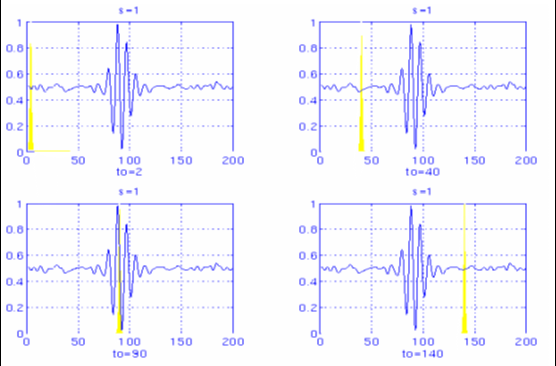
\includegraphics[width=0.6\textwidth]
	{images/chapter3/cwt-1}
	\caption{}
	\label{fig:cwt-1}
\end{figure}

The signal and the wavelet function are shown for four different values of tau. The signal is a truncated version of the signal shown in Figure . The scale value is 1, corresponding to the lowest scale, or highest frequency. Note how compact it is (the blue window). It should be as narrow as the highest frequency component that exists in the signal. Four distinct locations of the wavelet function are shown in the figure at to=2, to=40, to=90, and to=140. At every location, it is multiplied by the signal. Obviously, the product is nonzero only where the signal falls in the region of support of the wavelet, and it is zero elsewhere. By shifting the wavelet in time, the signal is localized in time, and by changing the value of s, the signal is localized in scale (frequency).
\begin{figure}[H]
    \centering
    \begin{subfigure}[b]{0.6\textwidth}
        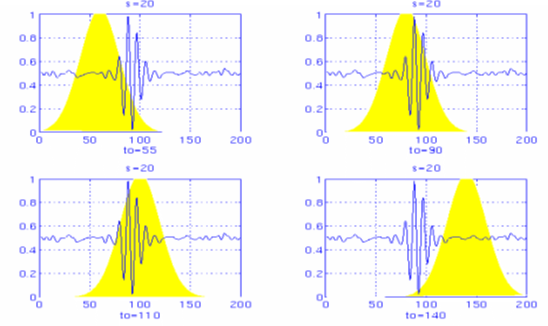
\includegraphics[width=\textwidth]
        {images/chapter3/cwt-scale-wide}
        \caption{}
        \label{fig:cwt-scale-wide}
    \end{subfigure}

    \begin{subfigure}[b]{0.6\textwidth}
        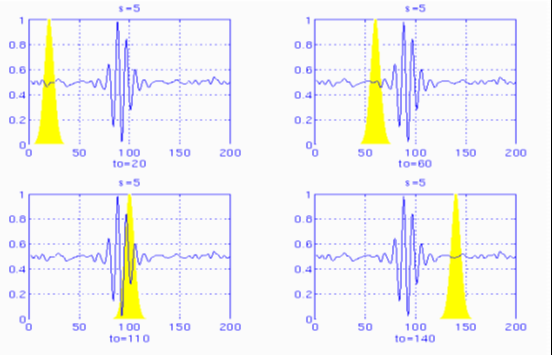
\includegraphics[width=\textwidth]
        {images/chapter3/cwt-scale-narrow}
        \caption{}
        \label{fig:cwt-scale-narrow}
    \end{subfigure}
    \caption{}
    \label{fig:cwt-scale-comparison}
\end{figure}

Figure \ref{fig:cwt-scale-comparison} illustrate the same process for the scales s=5 and s=20, respectively. Note how the window width changes with increasing scale (decreasing frequency). As the window width increases, the transform starts picking up the lower frequency components.
\subsection{Discrete Wavelet Transform}
Although the discretized continuous wavelet transform enables the computation of the continuous wavelet transform by computers, it is not a true discrete transform. As a matter of fact, the wavelet series is simply a sampled version of the CWT, and the information it provides is highly redundant as far as the reconstruction of the signal is concerned. This redundancy, on the other hand, requires a significant amount of computation time and resources. The discrete wavelet transform(DWT), on the other hand, provides sufficient information both for analysis and synthesis of the original signal, with a significant reduction in the computation time.
\par
The DWT is considerably easier to implement when compared to the CWT. The foundations of the DWT go back to 1976 when Crosier, Esteban, and Galand devised a technique to decompose discrete time signals. Crochiere, Weber, and Flanagan did a similar work on coding of speech signals in the same year. They named their analysis scheme as sub band coding. In 1983, Burt defined a technique very similar to sub band coding and named it pyramidal coding which is also known as multiresolution analysis. Later in 1989, Vetterli and Le Gall made some improvements to the sub band coding scheme, removing the existing redundancy in the pyramidal coding scheme. Subband coding is explained below.
\subsubsection{Sub-band Coding and The Multi-resolution Analysis}
The main idea is a time-scale representation of a digital signal is obtained using digital filtering techniques. Recall that the CWT is a correlation between a wavelet at different scales and the signal with the scale (or the frequency) being used as a measure of similarity. The continuous wavelet transform was computed by changing the scale of the analysis window, shifting the window in time, multiplying by the signal, and integrating over all times. In the discrete case, filters of different cutoff frequencies are used to analyze the signal at different scales. The signal is passed through a series of high pass filters to analyze the high frequencies, and it is passed through a series of low pass filters to analyze the low frequencies. 
\par
The resolution of the signal, which is a measure of the amount of detail information in the signal, is changed by the filtering operations, and the scale is changed by up sampling and down sampling (subsampling) operations. Subsampling a signal corresponds to reducing the sampling rate,or removing some of the samples of the signal. For example, subsampling by two refers to dropping every other sample of the signal. Subsampling by a factor n reduces the number of samples in the signal n times.
\par
The procedure starts with passing this signal (sequence) through a half band digital lowpass filter with impulse response h[n]. Filtering a signal corresponds to the mathematical operation of convolution of the signal with the impulse response of the filter. The convolution operation in discrete time is defined as,
\begin{equation*}
x[n]*h[n] = \sum_{k=-\infty}^{\infty} x[k].h[n-k]
\end{equation*}
A half band lowpass filter removes all frequencies that are above half of the highest frequency in the signal. For example, if a signal has a maximum of 1000 Hz component, then half band lowpass filtering removes all the frequencies above 500 Hz.
\par
The unit of frequency is of particular importance at this time. In discrete signals, frequency is expressed in terms of radians. Accordingly, the sampling frequency of the signal is equal to 2p radians in terms of radial frequency. Therefore, the highest frequency component that exists in a signal will be p radians, if the signal is sampled at Nyquist’s rate (which is twice the maximum frequency that exists in the signal); that is, the Nyquist’s rate corresponds to p rad/s in the discrete frequency domain. Therefore, using Hz is not appropriate for discrete signals. However, Hz is used whenever it is needed to clarify a discussion, since it is very common to think of frequency in terms of Hz. It should always be remembered that the unit of frequency for discrete time signals is radians.
\par
After passing the signal through a half band lowpass filter, half of the samples can be eliminated according to the Nyquist’s rule, since the signal now has a highest frequency of p/2 radians instead of p radians. Simply discarding every other sample will subsample the signal by two, and the signal will then have half the number of points. The scale of the signal is now doubled. Note that the lowpass filtering removes the high frequency information, but, leaves the scale unchanged. Only the subsampling process changes the scale. Resolution, on the other hand, is related to the amount of information in the signal, and therefore, it is affected by the filtering operations. Half band lowpass filtering removes half of the frequencies, which can be interpreted as losing half of the information. Therefore, the resolution is halved after the filtering operation. Note, however, the subsampling operation after filtering does not affect the resolution, since removing half of the spectral components from the signal makes half the number of samples redundant anyway. Half the samples can be discarded without any loss of information. In summary, the lowpass filtering halves the resolution, but leaves the scale unchanged. The signal is then subsampled by 2 since half of the number of samples are redundant. This doubles the scale. This procedure can mathematically be expressed as
\begin{equation*}
y[n] = \sum_{k=-\infty}^{\infty} h[k].x[2n-k]
\end{equation*}
Having said that, we now look how the DWT is actually computed: The DWT analyzes the signal at different frequency bands with different resolutions by decomposing the signal into a coarse approximation and detail information. DWT employs two sets of functions, called scaling functions and wavelet functions, which are associated with low pass and high pass filters, respectively. The decomposition of the signal into different frequency bands is simply obtained by successive high pass and lowpass filtering of the time domain signal. The original signal x[n] is first passed through a half band high pass filter g[n] and a lowpass filter h[n]. After the filtering, half of the samples can be eliminated according to the Nyquist’s rule, since the signal now has a highest frequency of p/2 radians instead of p. The signal can therefore be subsampled by 2, simply by discarding every other sample.
\par
This constitutes one level of decomposition and can mathematically be expressed as follows:
\begin{align*}
y_{high}[k] &= \sum_{n} x[n].g[2k-n] \\ 
y_{low}[k] &= \sum_{n} x[n].h[2k-n]
\end{align*}
where $y_{high}[k]$ and $y_{low}[k]$ are the outputs of the high pass and lowpass filters, respectively, after subsampling by 2. 
\par
This decomposition halves the time resolution since only half the number of samples now characterizes the entire signal. However, this operation doubles the frequency resolution, since the frequency band of the signal now spans only half the previous frequency band, effectively reducing the uncertainty in the frequency by half. The above procedure, which is also known as the subband coding, can be repeated for further decomposition. At every level, the filtering and subsampling will result in half the number of samples (and hence half the time resolution) and half the frequency band spanned (and hence double the frequency resolution). Figure \ref{fig:subband-algorithm} illustrates this procedure, where x[n] is the original signal to be decomposed, and h[n] and g[n] are lowpass and high pass filters, respectively. The bandwidth of the signal at every level is marked on the figure as "f".

\begin{figure}[!h]
	\centering
	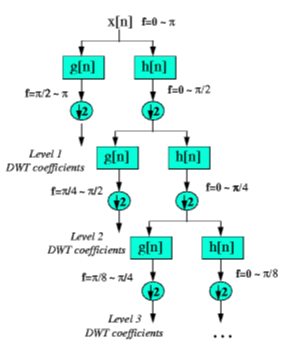
\includegraphics[width=0.4\textwidth]
	{images/chapter3/subband-algorithm}
	\caption{Subband Coding Algorithm.}
	\label{fig:subband-algorithm}
\end{figure}

\begin{figure}[!h]
	\centering
	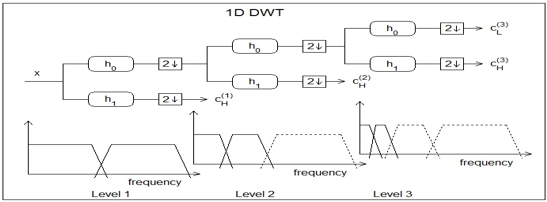
\includegraphics[width=.8\textwidth]
	{images/chapter3/subband-algorithm-2}
	\caption{}
	\label{fig:subband-algorithm-2}
\end{figure}

\begin{figure}[!h]
	\centering
	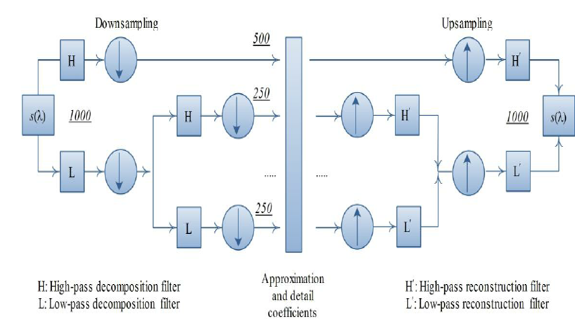
\includegraphics[width=.8\textwidth]
	{images/chapter3/subband-algorithm-3}
	\caption{}
	\label{fig:subband-algorithm-3}
\end{figure}

The DWT of the original signal is then obtained by concatenating all coefficients starting from the last level of decomposition (remaining two samples, in this case). The DWT will then have the same number of coefficients as the original signal. 
\par
The frequencies that are most prominent in the original signal will appear as high amplitudes in that region of the DWT signal that includes those particular frequencies. The difference of this transform from the Fourier transform is that the time localization of these frequencies will not be lost. However, the time localization will have a resolution that depends on which level they appear. If the main information of the signal lies in the high frequencies, as happens most often, the time localization of these frequencies will be more precise, since they are characterized by more number of samples. If the main information lies only at very low frequencies, the time localization will not be very precise, since few samples are used to express signal at these frequencies. This procedure in effect offers a good time resolution at high frequencies, and good frequency resolution at low frequencies. Most practical signals encountered are of this type. 
\par
The frequency bands that are not very prominent in the original signal will have very low amplitudes, and that part of the DWT signal can be discarded without any major loss of information, allowing data reduction. Figure 4.2 illustrates an example of how DWT signals look like and how data reduction is provided.
\par
One important property of the discrete wavelet transform is the relationship between the impulse responses of the high pass and lowpass filters. The high pass and lowpass filters are not independent of each other, and they are related by
\begin{equation*}
g[L-1-n] = (-1)^n .h(n)
\end{equation*}

where g[n] is the high pass, h[n] is the lowpass filter, and L is the filter length (in number of points). Note that the two filters are odd index alternated reversed versions of each other. Lowpass to high pass conversion is provided by the $(-1)^n$ term. Filters satisfying this condition are commonly used in signal processing, and they are known as the Quadrature Mirror Filters (QMF). The two filtering and subsampling operations can be expressed by
\begin{align*}
y_{high}[k] &= \sum_{n} x[n].g[-n+2k] \\ 
y_{low}[k] &= \sum_{n} x[n].h[-n+2k]
\end{align*}
The reconstruction in this case is very easy since half band filters form orthonormal bases. The above procedure is followed in reverse order for the reconstruction. The signals at every level are up sampled by two, passed through the synthesis filters g’[n], and h’[n] (high pass and lowpass, respectively), and then added. The interesting point here is that the analysis and synthesis filters are identical to each other, except for a time reversal. Therefore, the reconstruction formula becomes (for each layer)
\begin{equation*}
x[n] = \sum_{k=-\infty}^{\infty} \left [ \left ( y_{high}[k].g[-n+2k] \right ) + \left ( y_{low}[k].h[-n+2k] \right ) \right ]
\end{equation*}
However, if the filters are not ideal half band, then perfect reconstruction cannot be achieved. Although it is not possible to realize ideal filters, under certain conditions it is possible to find filters that provide perfect reconstruction. The most famous ones are the ones developed by Ingrid Daubechies, and they are known as Daubechies’ wavelets.
\par
Note that due to successive subsampling by 2, the signal length must be a power of 2, or at least a multiple of power of 2, in order this scheme to be efficient. The length of the signal determines the number of levels that the signal can be decomposed to. For example, if the signal length is 1024, ten levels of decomposition are possible.
\par 
Interpreting the DWT coefficients can sometimes be rather difficult because the way DWT coefficients are presented is rather peculiar. To make a real long story real short, DWT coefficients of each level are concatenated, starting with the last level.

\subsubsection{Wavelet Families}
\subsubsection{Haar Wavelet}
Is the first and simplest orthonormal wavelet basis. The Haar wavelet is conceptually simple, memory efficient, exactly reversible without the edge effects characteristic of other wavelets and computationally cheap. The Haar transform does not have overlapping windows,and reflects only changes between adjacent pixel pairs. it uses just two scaling and wavelet function coefficients, thus calculates pair wise averages and differences.
\begin{figure}[!h]
	\centering
	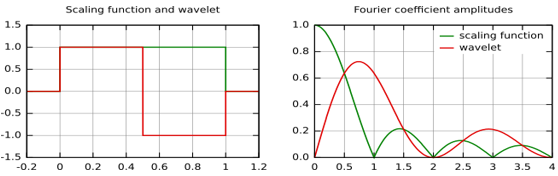
\includegraphics[width=0.8\textwidth]
	{images/chapter3/haar-wavelet}
	\caption{Haar wavelet}
	\label{fig:haar-wavelet}
\end{figure}

\subsubsection{Daubechies Wavelet}
family is the most popular wavelet family used for texture feature analysis, due to orthogonal and compact support abilities. The Daubechies wavelet uses overlapping windows, so the results reflect all changes between pixel intensities. Since Daubechies averages over more pixels, it is smoother than the Haar wavelet. The Daubechies D4 transform has four wavelet and scaling coefficients. The sum of the scaling function coefficients are also one, thus the calculation is averaging over four adjacent pixels.

\begin{figure}[!h]
	\centering
	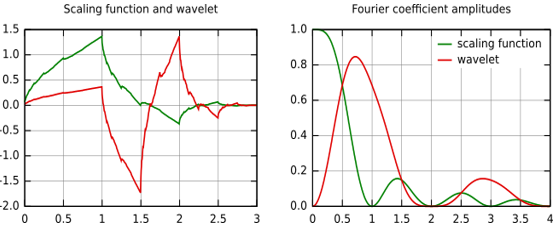
\includegraphics[width=0.75\textwidth]
	{images/chapter3/daubechies-4}
	\caption{Daubechies 4 wavelet}
	\label{fig:daubechies-4}
\end{figure}
\begin{figure}[!h]
	\centering
	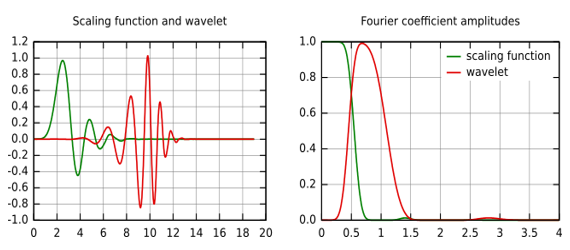
\includegraphics[width=0.75\textwidth]
	{images/chapter3/daubechies-20}
	\caption{Daubechies 20 wavelet.}
	\label{fig:daubechies-20}
\end{figure}
\begin{figure}[!h]
	\centering
	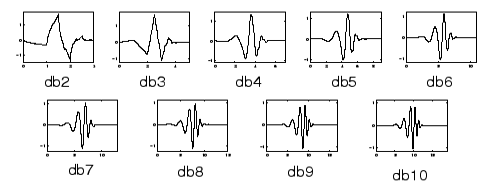
\includegraphics[width=0.6\textwidth]
	{images/chapter3/daubechies-1-10}
	\caption{Daubechies 2-10}
	\label{fig:daubechies-1-10}
\end{figure}

Applications of Wavelet Transform
\begin{enumerate}
\item Image Compression: JPEG 2000
\item Denoising noisy data
\item Edge and Corner Detection
\item Pattern recognition
\item Filter design
\item Analysis of the Electrocardiogram (ECG)
\end{enumerate}

\section{De-noising Using Wavelet Transform}
\subsection{Introduction}
Fourier transform based spectral analysis is the dominant analytical tool for frequency domain analysis. However, Fourier transform cannot provide any information of the spectrum changes with respect to time. Fourier transform assumes the signal is stationary, but speech signal is always non-stationary. To overcome this deficiency, a modified method-short time Fourier transform allows to represent the signal in both time and frequency domain through time windowing functions. The window length determines a constant time and frequency resolution. Thus, a shorter time windowing is used in order to capture the transient behaviour of a signal; we sacrifice the frequency resolution. The nature of the real speech signals is non-periodic and transient; such signals cannot easily be analysed by conventional transforms. So, an alternative mathematical tool – wavelet transform must be selected to extract the relevant time-amplitude information from a signal.
\subsection{Noise consideration}
A signal is unfortunately corrupted by various factors which effects as noise during acquisition. These noisy effects decrease the performance of visual and computerized analysis. It is clear that the removing of the noise from the signal facilitate the processing. The de-noising process can be described as to remove the noise while retaining and not distorting the quality of processed signal. The traditional way of de-noising to remove the noise from a signal or an image is to use a low or band pass filter with cut off frequencies. However the traditional filtering techniques are able to remove a relevant of the noise, they are incapable if the noise in the band of the signal to be analysed. Therefore, many de-noising techniques are proposed to overcome this problem.
\par
Because the origin and non-stationary of the noise infecting in  the signal, it is difficult to model it. Nevertheless, if the noise assumed as stationary, an empirically recorded signal that is corrupted by additive noise can be represented as;
\begin{equation*}
Y(i) = X(i) + \sigma \varepsilon(i)
\end{equation*}

Where $Y(i)$ noisy signal,  $X(i)$  is noise free actual signal and  $\varepsilon(i)$ are independently normal random variables and  $\sigma$ represents the intensity of the noise in $Y(i)$  . The noise is usually modelled as stationary independent zero-mean white Gaussian variables.
\par
When this model is used, the objective of noise removal is to reconstruct the original signal $X(i)$  from a finite set of $Y(i)$  values without assuming a particular structure for the signal. The usual approach to noise removal models noise as high frequency signal added to an original signal. These high frequencies can be bringing out using traditional Fourier transform, ultimately removing them by adequate filtering. This noise removal technique conceptually clear and efficient since depends only calculating DFT (Discrete Fourier Transform).
\par
However, there is some issue that must be under consideration. The most prominent having same frequency as the noise has important information in the original signal. Filtering out these frequency components will cause noticeable loss of information of the desired signal when considered the frequency representation of the original signal. It is clear that a method is required in order to conserve the prominent part of the signal having relatively high frequencies as the noise has. The wavelet based noise removal techniques have provided this conservation of the prominent part.

\subsection{Algorithm}
In Automatic 1-D De-noising, It performs an automatic 
de-noising process of a one-dimensional  signal  using wavelets  and  returns  a  de-noised  version of  input  signal  obtained  by  thresholding the  wavelet  coefficients.  The  De-noising objective  is  to  suppress  the  noise  part  of the  signal  and  to  recover  the  original one. The de-noising procedure proceeds in three steps:
\begin{enumerate}
\item Decomposition
\item Thresholding and threshold estimation techniques 
\item Reconstruction
\end{enumerate}

\begin{figure}[!h]
	\centering
	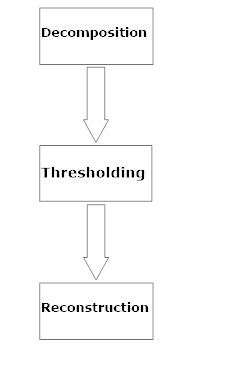
\includegraphics[width=0.3\textwidth]
	{images/chapter3/denoise-proc}
	\caption{de-noising procedure}
	\label{fig:denoise-proc}
\end{figure}

\subsubsection{Decomposition}
The signal is decomposed in ``approximation'' and ``detail'' coefficients at each level. This is made through a process that is equivalent to low-pass and high passes filtering, respectively, by using wavelet packet transform.

\subsubsection{Thresholding \& Threshold Estimation Techniques}
The simpler way to remove noise or to reconstruct the original signal from a contaminated signal, using the wavelet coefficients which are the result of decomposition in wavelet transform, is to eliminate the small coefficient associated to the noise. After updating the coefficients by removing the small coefficients assuming as noise, the original signal can be obtained by the reconstruction algorithm using the noise free coefficients. Because it is usually considered that the noise has high frequency coefficients, the elimination of the small coefficient generally applied on the detail coefficients after the decomposition. Indeed, the main idea of the wavelet de-noising to obtain the ideal components of the signal from the noisy signal requires the estimation of the noise level. The estimated noise level is used in order to threshold the small coefficient assumed as noise.

Thresholding can be applied by implementing either hard or soft thresholding method, which also called as shrinkage. In the hard thresholding, the wavelet coefficient below a give value are stetted to zero, while in soft thresholding the wavelet coefficient are reduced be a quantity to the thresh value.  The threshold value is the estimation of the noise level, which is generally calculated from the standard deviation of the detail coefficient. Figure 4 ??? indicates the two types of thresholding, which can be expressed analytically as
\begin{itemize}
\item Hard threshold
\begin{equation*}
y = \begin{cases}
x, & \left | x  \right | > \lambda \\ 
0, & \left | x  \right | < \lambda
\end{cases}
\end{equation*}
\item Soft threshold
\begin{equation*}
y = \text{sign}(x) \left ( \left | x \right | - \lambda \right )
\end{equation*}
\end{itemize}

Where $x$  is the input signal, $y$ is the signal after threshold and  $\lambda$ is the threshold value ,which is critical as the estimator leading to destruction, reduction, or increase in the value of a wavelet coefficient.

\begin{figure}[!h]
	\centering
	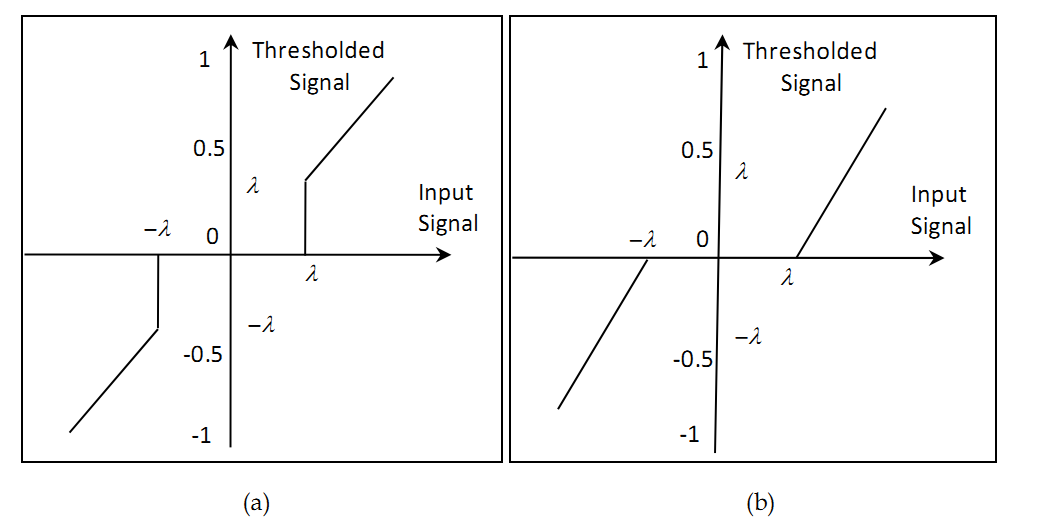
\includegraphics[width=0.8\textwidth]
	{images/chapter3/threshold-types}
	\caption{Threshold types: (a)hard, (b)Soft.}
	\label{fig:threshold-types}
\end{figure}

One important point in thresholding methods   is to find the appropriate value for the threshold. Actually, many approaches have   been proposed for calculating the threshold value. But, all the approaches require the estimation of   noise level. However the standard deviation of the data values may be used as an estimator, Donoho proposed a good estimator $\sigma$ for the wavelet de-noising given as;
\begin{equation}
\sigma = \frac{\text{median}(d (l-1,k))}{.6754}, \; \; k = 0, 1,...,2^{l-1} - 1
\label{eq:sigma-median}
\end{equation}
Where $l$ denotes the number of decomposition levels. As mentioned above, this median selection made on the detail coefficient of the analysed signal. 
the threshold estimator by Donoho is the  universal threshold, or global threshold, it uses a fixed threshold form given as;
\begin{equation*}
\lambda u = \sigma \sqrt{\log n}
\end{equation*}
Where $n$ denotes the length of the analysed signal and $\sigma$ is given by equation \ref{eq:sigma-median}. The advantage of this thresholding appears in software implementation due to easy to remember and coding.

\subsubsection{Reconstruction}
After  decomposing  the  signal  in approximate  and  detail  coefficients, threshold  value  is  selected  by  using threshold  selection  rule.  Then  by  using this  value,  thresholding  is  done  on detailed  coefficients.  After  detail coefficients  thresholding,  signal  is reconstructed  by  using  original approximation  coefficients  and  modified detail  coefficients.  Both hard and soft thresholding techniques are used   to compare the efficiency of the method. figure \ref{} illustrates the original noisy signal and the reconstructed signal.

\begin{figure}[!h]
    \centering
    \begin{subfigure}[b]{0.45\textwidth}
        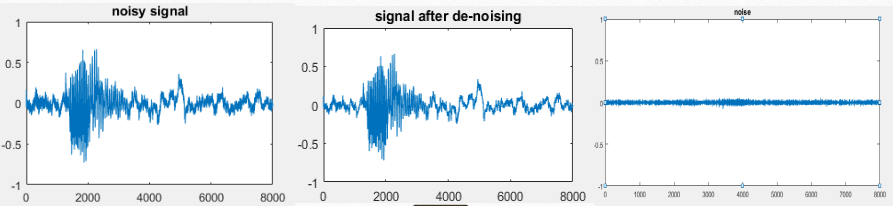
\includegraphics[width=\textwidth]
        {images/chapter3/comp-noisy-sig}
        \caption{original noisy signal}
        \label{fig:comp-noisy-sig}
    \end{subfigure}
    \hfill
    \begin{subfigure}[b]{0.45\textwidth}
        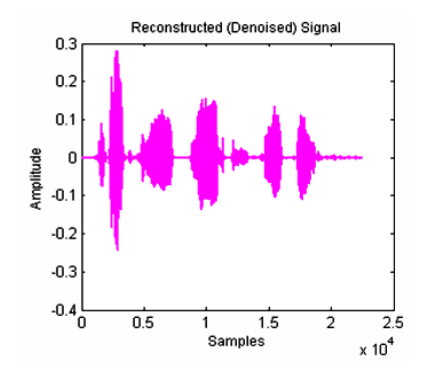
\includegraphics[width=\textwidth]
        {images/chapter3/comp-denoisy-sig}
        \caption{denoised signal.}
        \label{fig:comp-denoisy-sig}
    \end{subfigure}
    \caption{}
    \label{fig:comp-denoisy-noisy}
\end{figure}


\section{Linear Predictive Coding}
\subsection{Introduction}
There exist many different types of speech compression that make use of a variety of different techniques. However, most methods of speech compression exploit the fact that speech production occurs through slow anatomical movements and that the speech produced has a limited frequency range. The frequency of human speech production ranges from around 300 Hz to 3400 Hz.

Speech compression is often referred to as speech coding which is defined as a method for reducing the amount of information needed to represent a speech signal. Most forms of speech coding are usually based on a lossy algorithm. Lossy algorithms are considered acceptable when encoding speech because the loss of quality is often undetectable to the human ear. There are many other characteristics about speech production that can be exploited by speech coding algorithms. One fact that is often used is that period of silence take up greater than 50\% of conversations. An easy way to save bandwidth and reduce the amount of information needed to represent the speech signal is to not transmit the silence.

Another fact about speech production that can be taken advantage of is that mechanically there is a high correlation between adjacent samples of speech. Most forms of speech compression are achieved by modelling the process of speech production as a linear digital filter. The digital filter and its slow changing parameters are usually encoded to achieve compression from the speech signal. Linear Predictive Coding (LPC) is one of the methods of compression that models the process of speech production. Specifically, LPC models this process as a linear sum of earlier samples using a digital filter inputting an excitement signal. An alternate explanation is that linear prediction filters attempt to predict future values of the input signal based on past signals. LPC models speech as an autoregressive process, and sends the parameters of the process as opposed to sending the speech itself.

Speech coding or compression is usually conducted with the use of voice coders or vocoders. There are two types of voice coders: waveform-following coders and model-base coders. Waveform following coders will exactly reproduce the original speech signal if no quantization errors occur. Model-based coders will never exactly reproduce the original speech signal, regardless of the presence of quantization errors, because they use a parametric model of speech production which involves encoding and transmitting the parameters not the signal. LPC vocoders are considered model-based coders which means that LPC coding is lossy even if no quantization errors occur. All vocoders, including LPC vocoders, have four main attributes: bit rate, delay, complexity, quality.

Any voice coder, regardless of the algorithm it uses, will have to make trade-offs between these different attributes. The first attribute of vocoders, the bit rate, is used to determine the degree of compression that a vocoder achieves. Uncompressed speech is usually transmitted at 64 kb/s using 8 bits/sample and a rate of 8 kHz for sampling. Any bit rate below 64 kb/s is considered compression. The linear predictive coder transmits speech at a bit rate of 2.4 kb/s, an excellent rate of compression. Delay is another important attribute for vocoders that are involved with the transmission of an encoded speech signal. Vocoders which are involved with the storage of the compressed speech, as opposed to transmission, are not as concern with delay. The general delay standard for transmitted speech conversations is that any delay that is greater than 300 ms is considered unacceptable. The third attribute of voice coders is the complexity of the algorithm used. The complexity affects both the cost and the power of the vocoder. Linear predictive coding because of its high compression rate is very complex and involves executing millions of instructions per second. LPC often requires more than one processor to run in real time. The final attribute of vocoders is quality. Quality is a subjective attribute and it depends on how the speech sounds to a given listener. One of the most common test for speech quality is the absolute category rating (ACR) test. This test involves subjects being given pairs of sentences and asked to rate them as excellent, good, fair, poor, or bad.

Linear predictive coders sacrifice quality in order to achieve a low bit rate and as a result often sound synthetic. The general algorithm for linear predictive coding involves an analysis or encoding part and a synthesis or decoding part. In the encoding, LPC takes the speech signal in blocks or frames of speech and determines the input signal and the coefficients of the filter that will be capable of reproducing the current block of speech. This information is quantized and transmitted. In the decoding, LPC rebuilds the filter based on the coefficients received. The filter can be thought of as a tube which, when given an input signal, attempts to output speech.

\subsection{LPC Model}

\begin{figure}[h!]
\centering
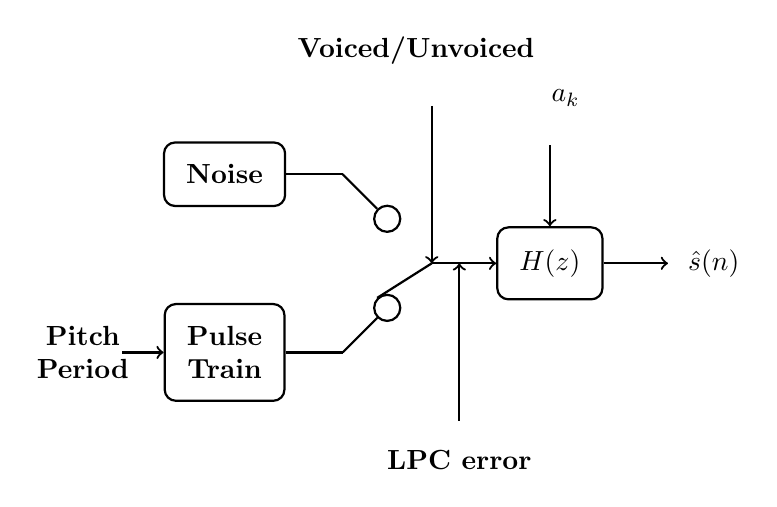
\begin{tikzpicture}[
node/.style={rectangle, draw=black, thick, rounded corners, inner sep=8pt, font=\bfseries},
circlenode/.style={circle, draw=black, thick, radius=1cm},
]
%Nodes
\node[node, align=center] (filter) {$H(z)$};
\node[coordinate, left of=filter, node distance=1.15cm] (amp) {};
\node[coordinate, below of=amp, node distance=2cm] (ampl) {};
\node[coordinate, above of=filter, node distance=1.5cm] (coefficients) {};
\node[coordinate, right of=filter, node distance=1.5cm] (output) {};
\node[coordinate, left of=filter, node distance=1.5cm] (prefilter) {};
\node[coordinate, above of=prefilter, node distance=2cm] (flag) {};
\node[circlenode, below left of=prefilter, node distance=0.8cm] (keybottom) {};
\node[circlenode, above left of=prefilter, node distance=0.8cm] (keytop) {};
\node[coordinate, below left of=keybottom, node distance=0.8cm] (posttrain) {};
\node[coordinate, above left of=keytop, node distance=0.8cm] (postnoise) {};
\node[node, node distance=1.5cm, left of=postnoise] (noise) {Noise};
\node[node, align=center, node distance=1.5cm, left of=posttrain] (train) {Pulse\\Train};
\node[coordinate, left of=train, node distance=1.3cm] (pitch) {};
 
%Lines
\draw[->, thick] (prefilter.east) -- (filter.west);
\draw[thick] (keybottom.north west) -- (prefilter.west);
\draw[thick] (postnoise.south) -- (keytop.north west);
\draw[thick] (posttrain.north) -- (keybottom.south west);
\draw[thick] (noise.east) -- (postnoise.west);
\draw[thick] (train.east) -- (posttrain.west);
\draw[->, thick] (filter.east) node[xshift=14mm, font=\bfseries]{$\hat{s}(n)$} -- (output.west);
\draw[->, thick] (coefficients.south) node[yshift=6mm , xshift=2mm, font=\bfseries, align=center]{$a_k$} -- (filter.north);
\draw[->, thick] (flag.south) node[yshift=7mm , xshift=-2mm, font=\bfseries, align=center]{Voiced/Unvoiced} -- (prefilter.north);
\draw[->, thick] (pitch.east) node[font=\bfseries, xshift=-5mm, align=center]{Pitch \\ Period} -- (train.west);
\draw[->, thick] (ampl.north) node[font=\bfseries, yshift=-5mm]{LPC error} -- (amp.south);

\end{tikzpicture}
\caption{LPC source-filter model}
\label{fig:lpc_model}
\end{figure}

Linear Prediction is a model based on human speech
production. It utilizes a conventional source-filter model, in which the glottal, vocal tract, and lip radiation transfer functions are integrated into one all-pole filter that
simulates acoustics of the vocal tract. The source is excited by noise in case of unvoiced speech, and is excited by a train of pulses in case of voiced speech. The LPC coefficients are the poles of the filter and the error is used for the gain. Figure \ref{fig:lpc_model}, shows a block diagram of the LPC model.

The principle behind the use of LPC is to minimize the sum of the squared differences between the original speech signal and the estimated speech signal over a finite duration. This could be used to give a unique set of predictor coefficients. These predictor coefficients are estimated every frame, which is normally 20 ms long. The predictor coefficients are represented by $a_k$.

The transfer function of the time varying
digital filter is given by
\begin{equation*}
H(z) = \frac{1}{1-\sum_{k=1}^{p} a_k z^{-k}}
\end{equation*}
Where k=1 to p, which will be 10 for the LPC-10 algorithm and 18 for the improved algorithm that is utilized. Levinsion-Durbin recursion will be utilized to compute the required parameters for the auto-correlation method. 

The LPC analysis of each frame also involves the decision-making process of voiced or unvoiced. A pitch-detecting algorithm is employed to determine correct pitch period. It is
important to re-emphasis that the pitch, gain and coefficient parameters will be varying with time from one frame to another. Figure \ref{fig:lpc_analysis_stages} shows analysis' stages.

\begin{figure}[h!]
\centering
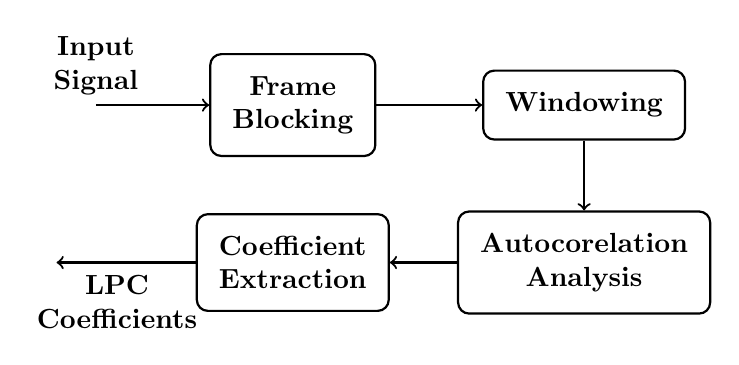
\begin{tikzpicture}
[node/.style={rectangle, draw=black, thick, rounded corners, inner sep=8pt, font=\bfseries}]

%Nodes
\node[node] (feature) {Windowing};
\node[node, left of= feature, node distance=3.7cm, align=center] (process) {Frame\\Blocking};
\node[coordinate, left of=process, node distance=2.5cm] (input) {};
\node[node, below of=feature, node distance=2cm, align=center] (classifier) {Autocorelation\\Analysis};
\node[node, left of=classifier, node distance=3.7cm, align=center] (model) {Coefficient\\Extraction};
\node[coordinate, left of=model, node distance=3cm] (output) {};
 
%Lines
\draw[->, thick] (input.east) node[yshift=5mm, font=\bfseries, align=center]{Input\\Signal} -- (process.west);
\draw[->, thick] (process.east) -- (feature.west);
\draw[->, thick] (feature.south) -- (classifier.north);
\draw[->, thick] (classifier.west) -- (model.east);
\draw[->, thick] (model.west) node[yshift=-5mm, xshift=-10mm, font=\bfseries, align=center]{LPC\\Coefficients} -- (output.east);

\end{tikzpicture}
\caption{Stages of LPC Analysis}
\label{fig:lpc_analysis_stages}
\end{figure}

\subsection{LPC Analysis}
Speech analysis based on linear predictive coding (LPC) has had a successful history for more than 30 years. The term "linear prediction" refers to the mechanism of using a linear combination of the past time-domain samples, $s[n-1]$, $s[n-2]$, ..., $s[n-M]$, to approximate or to "predict" the current time-domain sample $s[n]$:
\begin{equation} \label{eq:lpc_shat}
s[n]\approx \hat{s}[n] = -\sum_{i=1}^{M}a_i s[n-i],
\end{equation}
where $\hat{s}[n]$ is called the predicted sample, and $a_i, i = 1,2,...,M$ are called predictor or LPC coefficients. If the prediction is accurate, then a small number of LPC coefficients $a_1, a_2, ..., a_M$, can be used to efficiently represent or to "code" a long sequence of the signal $s[n]$. 

Linear prediction expressed in the time-domain by Eq. \ref{eq:lpc_shat} is the all-pole modelling, where the "prediction" operation was treated as a discrete-time linear system transformation. In the time-series analysis literature in statistics, the linear prediction of Eq. \ref{eq:lpc_shat} is also called an autoregressive model.

Define the sampled error for the prediction as
\begin{equation} \label{eq:lpc_error}
e[n] = s[n]-\hat{s}[n] = s[n] + \sum_{i=1}^{M}a_i s[n-i] = \sum_{i=0}^{M}a_i s[n-i],
\end{equation}
where $a_0 = 1$. Taking the $z$-transform on Eq. \ref{eq:lpc_error}, we obtain
\begin{equation} \label{eq:lpc_errorz}
E(z) = S(z) + \sum_{i=1}^{M} a_i S(z) z^{-i} = S(z)\left [ 1 + \sum_{i=1}^{M} a_i z^{-i} \right ] = S(z) A(z)
\end{equation}
where
\begin{equation*} \label{eq:lpc_az}
A(z) = 1 + \sum_{i=1}^{M} a_i z^{-i} = \sum_{i=0}^{M} a_i z^{-i}
\end{equation*}
Eq. \ref{eq:lpc_errorz} can be equivalently written as
\begin{equation*} \label{eq:lpc_sz}
S(z) = E(z) \frac{1}{A(z)}
\end{equation*}

This shows that the speech signal can be viewed as the output of an all-pole digital filter, whose transfer function is
\begin{equation*} \label{eq:lpc_filter_tf}
\frac{1}{A(z)}
\end{equation*}
and the input to the filter is the LPC error signal $e[n]$. This (forward) filtering view of LPC analysis can be used in interpret Eq. \ref{eq:lpc_errorz} as inverse filtering. That is, if we pass the speech signal $s[n]$ as input into an inverse filter whose transfer function is $A(z)$, then the output of the inverse filter will be the error signal $e[n]$. $A(z)$ acts as the inverse of the synthesis filter that creates $S(z)$.

\subsection{Least-squares estimate of LPC coefficients}
One key importance of the LPC analysis is that the LPC coefficients, $a_1, a_2, ..., a_M$, which are the parameters of the LPC inverse filter $A(z)$, can be determined directly from the speech signal $s[n]$. The least-squares criterion is mathematically tractable, computationally efficient, and it has been shown to be highly effective in speech analysis.

Under the least-squares optimization criterion, the total squared error is defined by

\begin{equation}
\varepsilon = \sum_{n=n_0}^{n_1} e^2[n],
\end{equation}

where $n_0$ and $n_1$ are summation limits, or the sample range over which the optimization is carried out. Substituting Eq. \ref{eq:lpc_error}, we have

\begin{equation*}
\varepsilon = \sum_{n=n_0}^{n_1} \left [ \sum_{i=0}^{M} a_i s[n-i] \right ]^2 = \sum_{n=n_0}^{n_1} \sum_{i=0}^{M} \sum_{j=0}^{M} a_i s[n-i] s[n-j] a_j = \sum_{i=0}^{M} \sum_{j=0}^{M} a_i c_{ij} a_j,
\end{equation*}

where

\begin{equation*}
c_{ij} = \sum_{n=n_0}^{n_1} s[n-i] s[n-j],
\end{equation*}

To minimize $\varepsilon$ with respect to the LPC coefficients $a_1, a_2, ..., a_M$, we set the partial derivatives to zero and solve the resulting equations. This gives
\begin{equation*}
\frac{\partial \varepsilon }{\partial a_k} = 2 \sum_{i=0}^{M} a_i c_{ij} = 0
\end{equation*}

Since $a_0 = 1$, this becomes the following celebrated normal equation:
\begin{equation*}
\sum_{i=1}^{M} a_i c_{ik} = -c_{0k}, k = 1, 2,..., M
\end{equation*}


\section*{References}
\begin{enumerate}
\item Ramesh    Babu.N "Speech Recognition using MFCC and DTW " Conference    Paper -1st Int. Conf. on Advances in Electrical Engineering, At VIT, Vellore, India January 2014, link: https://www.researchgate.net/publication/260762671
\item http://practicalcryptography.com/miscellaneous/machine-learning/guide-mel-frequency-cepstral-coefficients-mfccs/
\item Shikha Gupta1, Jafreezal Jaafar2, Wan Fatimah wan Ahmad3  and Arpit Bansal4 "FEATURE EXTRACTION USING MFCC "Signal \& Image Processing : Signal \& Image Processing, An International Journal (SIPIJ) Vol.4, No.4, August 2013
\item A. Graps, “An Introduction to Wavelets,” IEEE Computational Sciences and Engineering, vol. 2, no.2, pp 50-61, 1995.
\item W. H. Press, et. al., Numerical Recipes in C: the Art of Scientific Computing, 2nd. ed., pp. 591-606, Cambridge University Press, 1992.
\item The essential guide to image processing : ALBOVIK
\item Slavy G. Mihov, Ratcho M. Ivanov, Angel N. Popov, Denoising Speech Signals by Wavelet Transform, ANNUAL JOURNAL OF ELECTRONICS,January 2009
\item Burhan Ergen (2012). Signal and Image Denoising Using Wavelet Transform, Advances in Wavelet Theory and Their Applications in Engineering, Physics and Technology, Dr.Dumitru Baleanu (Ed.), ISBN: 978-953-51-0494-0, InTech, Available from: http://www.intechopen.com/books/advances-in-wavelet-theory-and-their-applications-in-engineering-physics-and-technology/wavelet-signal-and-image-denoising
\item V.S.R Kumari1, Dileep Kumar Devarakonda2, A Wavelet Based Denoising of Speech Signal, International Journal of Engineering Trends and Technology (IJETT) – Volume 5 number 2 - Nov 2013
\item Jeremy Bradbury, Linear Predictive Coding, Florida Institute of Technology, 2000.
\item Li Deng and Douglas O'Shaughnessy, Speech Processing: A Dynamic and Optimization-Oriented Approach, CRC Press, 2003.
\item Urmila Shrawankar, Techniques for Feature Extraction in Speech Recognition System: A Comparative Study, SGB Amravati University.
\end{enumerate}










































































%%%%%%%%%%%%%%%%%%%%%%%%%%%%%%%%%%%%%%%%%%%%%%%%%%%%%%%%%%%%%%%%%%%%%%%%%%%%%%%%%%%%%%%%%%%%%%%%%%%%%%%%%%%%%%%%%%%%%%%%%%%%%%%%%%%%%%%%%%%%%%%%%%%%%%%%%%%%%%%%%%%%%%%%%%%%%%%%%%%%%%%%%%%%%%% CHAPTER 4 %%%%%%%%%%%%%%%%%%%%%%%%%%%%%%%%%%%%%%%%%%%%%%%%%%%%%%%%%%%%%%%%%%%%%%%%%%%%%%%%%%%%%%%%%%%%%%%%%%%%%%%%%%%%%%%%%%%%%%%%%%%%%%%%%%%%%%%%%%%%%%%%%%%%%%%%%%%%%%%%%%%%%%%%%%%%%%%%%%%%%%%%%%%%






















































































\chapter{Classification}
\section{Neural Network}
\subsection{History}
The study of the human brain is hundreds of years old. With the advent of modern electronics, it was only natural to try to harness this thinking process. The first step towards artificial neural networks came in 1943 when Warren McCulloch, a neurophysiologist, and a young mathematician, Walter Pitts, wrote a paper on how neurons might work. They modelled a simple neural network with electrical circuits.
\par
Reinforcing this concept of neurons and how they work was a book written by Donald Hebb. {\itshape The Organization of Behaviour} was written in 1949. It pointed out that neural pathways are strengthened each time they are used.
\par
In 1956 the Dartmouth Summer Research Project on Artificial Intelligence provided a boost to both artificial intelligence and neural networks. One of the outcomes of this process was to stimulate research in both the intelligent side, AI, as it is known throughout the industry, and in the much lower level neural processing part of the brain.
\par
In 1959, Bernard Widrow and Marcian Hoff of Stanford developed models they called Adaline and Madaline. These models were named for their use of multiple adaptive linear elements. Madaline was the first neural network to be applied to a real world problem. It is an adaptive filter which eliminates echoes on phone lines. This neural network is still in commercial use.
\par
In 1982 several events caused a renewed interest. John Hopfield of Caltech presented a paper to the national Academy of Sciences. Hopfield's approach was not to simply model brains but to create useful devices. With clarity and mathematical analysis, he showed how such networks could work and what they could do. Yet, Hopfield's biggest asset was his charisma. He was articulate, likeable, and a champion of a dormant technology.
\par
By 1985 the American Institute of Physics began what has become an annual meeting - Neural Networks for Computing. By 1987, the Institute of Electrical and Electronic Engineers (IEEE) first International Conference on Neural Networks drew more than 1,800 attendees.
\par
By 1989 at the Neural Networks for Defence meeting Bernard Widrow told his audience that they were engaged in World War IV, ``World War III never happened," where the battlefields are world trade and manufacturing.
\par
Thousands of neural networks have been applied in hundreds of fields in the many years since the DARPA report was written. A list of some of those applications follows:
\begin{enumerate}
\item {\bfseries Automotive:} Auto-mobile automatic guidance systems, fuel injector control, automatic braking systems, misfire detection, virtual emission sensors, warranty activity analysers.
\item {\bfseries Electronics:} Code sequence prediction, integrated circuit chip layout, process control, chip failure analysis, machine vision, voice synthesis, non-linear modelling.
\item {\bfseries Robotics:} Trajectory control, forklift robot, manipulator controllers, vision systems, autonomous vehicles.
\item {\bfseries Speech:} Speech recognition, speech compression, vowel classification, text to speech synthesis.
\item {\bfseries Telecommunications:} Image and data compression, automated information services, real-time translation of spoken language, customer payment processing systems.
\end{enumerate}
and many other applications.

\subsection{Biological Neural Networks}
The neuron can be separated into three major parts: the cell body (soma), the dendrites, and the axon. The dendrites contain thin lines that receive signals from surrounding neurons. Each branch of a dendrite is connected to a single neuron through the small connection of a synapse. A signal of either chemical diffusion or electrical impulses is transmitted through the thin cylinder of the axon, through the synapse connection, and into the connected dendrite of specific neuron.
\par
When the neurons are performing a specific task, a certain number of neurons must be used in order to complete it. Input signals are distributed across the required neurons of different strengths or frequencies. All of these input signals are then added together and processed by a threshold function. The function then produces an output signal processed by all of the inputs. It is this entire function that makes up how humans are able to learn new information and process problems. While the processing time of $1ms$ per cycle, or a transmission speed of $0.6ms$ to $120ms$ is slower than a modern computer, the capability of learning information to recognize and solve various problems is the reason why the neural network of a human brain is an excellent structure for artificial intelligence Fig \ref{fig:biological_neuron}.

\begin{figure}[ht]
	\centering
	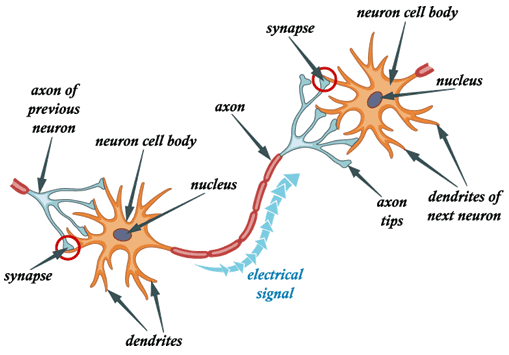
\includegraphics[width=0.8\textwidth]
	{images/chapter4/biological_neuron}
	\caption{simplified biological neurons.}
	\label{fig:biological_neuron}
\end{figure}

\subsection{Artificial Neural Networks}
In the late 19th century a neuroscientist named Santiago Ramón y Cajal conducted studies on the human nervous system. Cajal discovered that the human nervous system was actually comprised of the discrete neurons that communicated with signals passed through axons, dendrites and synapses . This discovery led to further research that identified different types of neurons, as well as the types of signals that were being passed between them. Neurobiologists were finding it very difficult however, to understand how the neurons were working together to achieve such a high level of functionality.
\par
It was not until the advancement of modern computing allowed researchers to be able to build working models of neural systems. These systems gave a better understanding of how the neural system of the brain functioned. Warren McCulloch and Walter Pitts created an early model of an artificial neuron in 1943. This model became known as a linear binary threshold gate. With a series of given inputs, a sum would be calculated against weight values normalized in the range of either (0, 1) or (-1, 1) and then associated with a specific input. Given a certain threshold, the output would be one of two classes in binary based on whether the sum exceeded the threshold or not as in Fig \ref{fig:artificial_neuron}.

\begin{figure}[ht]
	\centering
	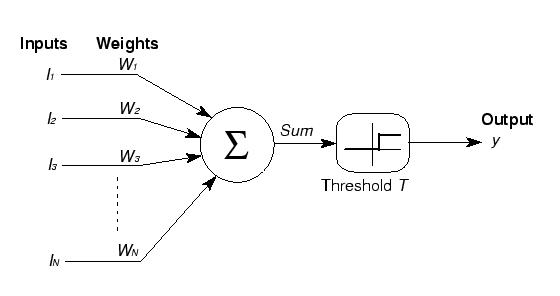
\includegraphics[width=0.8\textwidth]
	{images/chapter4/artificial_neuron}
	\caption{Symbolic Illustration of Linear Threshold Gate.}
	\label{fig:artificial_neuron}
\end{figure}

With this model of an artificial neuron it was now proven that systems of neurons that were assembled into a finite state automaton could compute any arbitrary function, when given suitable values for the weights between the neurons. Researchers went even further by implementing learning procedures that were capable of automatically finding appropriate weight values, which enabled a network to compute any specific function. As the years passed and more research was performed. Basic attributes of neural networks were defined, different training methods were created, and new network architectures were implemented.

\subsection{Fundamentals of Neural Networks}
While there are many different architectures of neural networks, each one of these systems contain similar basic attributes. These attributes are processing units, weights, a computation method and a training method, as equation \ref{eq:first_neuron}  which describes figure \ref{fig:single_input_neuron}.

\begin{equation}
n = \sum (w \times p) + b
\label{eq:first_neuron}
\end{equation}

\subsubsection{Processing Units}
A neural network system is made up of a specific number of processing units that represent neurons in a human brain. These units are typically divided into different groups. Some units represent the input units that receive the data to process, for example numerical values representing an image. Units that are hidden inside the neural network work to manipulate and transform the input information. The final group of units that can be known as output units represent the decision of the neural network.
\par
Each neuron that receives data performs a defined function. The results of this function are then shared with connected neurons. The sharing of this value is called the activation value. This value determines whether the receiving neuron will be activated or if it will remain inactive. There are several different activation functions that approximate the activation value to either [1 to 0], or [1 to -1] as in figure \ref{fig:activation_functions}.

\begin{figure}[ht]
	\centering
	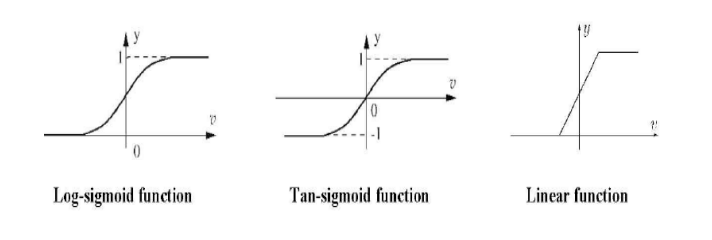
\includegraphics[width=1\textwidth]
	{images/chapter4/activation_functions}
	\caption{activation functions.}
	\label{fig:activation_functions}
\end{figure}

\subsubsection{Weights}
The processing units in a neural network must be connected in some way. These connections between neurons are displayed as lines in neural network diagrams. Each connection is assigned a value of a weight. These weights represent how influential a neuron is to another connected neuron. Typically the input from a neuron is multiplied by the weight of the connection that is sending the data. This value is then entered into the activation function of the network. If the value exceeds the given threshold of the activation function then the neuron will be activated, otherwise the neuron will remain inactive.

\subsubsection{Computation Method}
A neural network uses what is called a threshold logic unit in order to perform the required computations stated above. This unit is an object that takes all of the different inputs from connected neurons, sums them together, and then uses the activation function to determine a correct output. This output is then either sent to the output layer of the network, or onto the next connected neuron in another hidden layer.

\subsubsection{Training Method}
In order for a neural network to perform efficiently and correctly it must be able to adapt its weights in order to achieve desired outputs for any input. The training process of a neural network is extremely important in order for the network to replicate a human brain being able to learn and respond to new information. This process involves iterating inputs of training data into the neural network. With some neural networks there will be a given desired output along with this training data. Each time the data gets into the neural network, the weights of the connections between the neurons may be updated in order to achieve the desired output. There are several different techniques to training neural networks, each one being appropriate for different problems.

\subsection{Neuron Model}
\subsubsection{Single-Input Neuron}
A single-input neuron is shown in figure \ref{fig:biological_neuron}. The scalar input $(p)$ is multiplied by the scalar weight $(w)$ to form $(wp)$ , one of the terms that is sent to the summer. The other input, $(1)$ , is multiplied by a bias $(b)$ and then passed to the summer. The summer output $(n)$, often referred to as the net input, goes into a transfer function $(f)$, which produces the scalar neuron output $(a)$. Some authors use the term ``activation function'' rather than transfer function and ``offset'' rather than bias. If we relate this simple model back to the biological neuron that we discussed, the weight $w$ corresponds to the strength of a synapse, the cell body is represented by the summation and the transfer function, and the neuron output a represents the signal on the axon as in figure \ref{fig:single_input_neuron}.

\begin{figure}[ht]
	\centering
	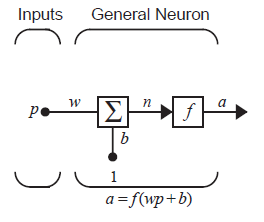
\includegraphics[width=0.35\textwidth]
	{images/chapter4/single_input_neuron}
	\caption{single-input nueron.}
	\label{fig:single_input_neuron}
\end{figure}

The neuron output is calculated as
\begin{equation*}
a = f(wp + b)
\end{equation*}
The actual output depends on the particular transfer function that is chosen. The bias is much like a weight, except that it has a constant input of $1$. $w$ and $b$ are both adjustable scalar parameters of the neuron. Typically the transfer function is chosen by the designer and then the parameters $w$ and $b$ will be adjusted by some learning rule so that the neuron input/output relationship meets some specific goal.

\subsubsection{Multiple-Input Neuron}
Typically, a neuron has more than one input. A neuron with $R$ inputs is shown in Fig 4.5. The individual inputs $P_1$, $P_2$, ...$P_R$ are each weighted by corresponding elements $W_{1,1}$, $W_{1,2}$, ...$W_{1,R}$ of the weight matrix $\mathbf{W}$.

\begin{figure}[ht]
	\centering
	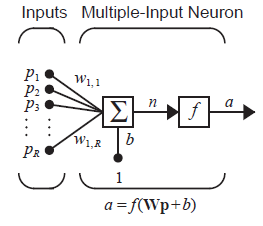
\includegraphics[width=0.35\textwidth]
	{images/chapter4/multiple_input_neuron}
	\caption{multiple-input neuron.}
	\label{fig:multiple_input_neuron}
\end{figure}

The neuron has a bias $b$, which is summed with the weighted inputs to form the net input $n$:
\begin{equation*}
n = W_{1,1}P_{1} + W_{1,2}P_{2} + ... + W_{1,R}P_{R} + b
\end{equation*}
This expression can be written in matrix form:
\begin{equation*}
n = \mathbf{Wp} + b
\end{equation*}
where the matrix $\mathbf{W}$ for the single neuron case has only one row. Now the neuron output can be written as
\begin{equation*}
a = f(\mathbf{Wp} + b)
\end{equation*}

\subsection{Neurons Architecture}
Commonly one neuron, even with many inputs, may not be sufficient. We might need five or ten, operating in parallel, in what is called a ``layer.'' This concept of a layer is discussed below.

\subsubsection{A Layer of Neurons}
Single-layer network of $S$ neurons is shown in figure \ref{fig:layer_neurons}. Each of the $R$ inputs is connected to each of the neurons and that the weight matrix now has $S$ rows.

\begin{figure}[!h]
	\centering
	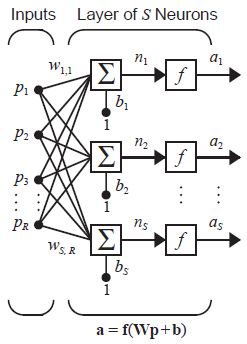
\includegraphics[width=0.35\textwidth]
	{images/chapter4/layer_neurons}
	\caption{layer of $S$ neurons.}
	\label{fig:layer_neurons}
\end{figure}

The layer includes the weight matrix, the summers, the bias vector $\mathbf{b}$, the transfer function boxes and the output vector.
\par
Each element of the input vector $\mathbf{p}$ is connected to each neuron through the weight matrix $\mathbf{W}$. Each neuron has a bias $b_i$, a summer, a transfer function and an output $a_i$. Taken together, the outputs form the output vector $\mathbf{a}$. It is common for the number of inputs to a layer to be different from the number of neurons i.e. $R \neq S$.
\par
Do all the neurons in a layer must have the same transfer function? The answer is no; you can define a single (composite) layer of neurons having different transfer functions by combining two of the networks shown above in parallel. Both networks would have the same inputs, and each network would create some of the outputs.
\par
The input vector elements enter the network through the weight matrix $\mathbf{W}$:
\begin{equation*}
\mathbf{W} = \begin{bmatrix}
w_{1,1} & w_{1,2} & ... & w_{1,R} \\ 
w_{2,1} & w_{2,2} & ... & w_{2,R} \\ 
 \vdots & \vdots & \ddots & \vdots \\ 
w_{S,1} & w_{S,2} & ... & w_{S,R}\\ 
\end{bmatrix}
\end{equation*}

Row indices of the elements of matrix $\mathbf{W}$ indicate the destination neuron associated with that weight, while the column indices indicate the source of the input for that weight. Thus, the indices in $w_{3,2}$ say that this weight represents the connection to the third neuron from the second source.

\subsubsection{Multiple Layers of Neurons}
Now consider a network with several layers. Each layer has its own weight matrix $\mathbf{W}$, its own bias vector $\mathbf{b}$, a net input vector $\mathbf{n}$ and an output vector $\mathbf{a}$. This is shown in the three-layer network shown in figure \ref{fig:three_layer_network}.
\begin{figure}[!h]
	\centering
	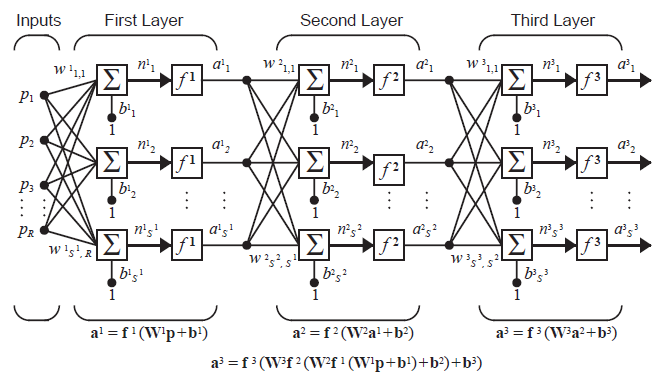
\includegraphics[width=1\textwidth]
	{images/chapter4/three_layer_network}
	\caption{three-layer network.}
	\label{fig:three_layer_network}
\end{figure}

Multi-layer networks are more powerful than single-layer networks. For instance, a two-layer network having a sigmoid first layer and a linear second layer can be trained to approximate most functions arbitrarily well. Single layer networks cannot do this. We should say something about the use of biases. One can choose neurons with or without biases. The bias gives the network an extra variable, and so you might expect that networks with biases would be more powerful than those without, and that is true. Note, for instance, that a neuron without a bias will always have a net input n of zero when the network inputs p are zero. This may not be desirable and can be avoided by the use of a bias.

\subsection{Neural Network Structures}
Artificial neural networks can be classified in two significant groups, feed-forward networks and recurrent networks.
\subsubsection{Feed-forward Neural Networks}
A feed-forward network is a directed and weighted graph that contains no loops. The input neurons contain no connection leading to them, and the output neurons contain no connections leading away from them. As the values of the input nodes are set, using the threshold logic unit, all other nodes in the network can set their values as well. A feed-forward neural network can either be a single layer network as or a multilayer network as in figure \ref{fig:feed-forward}.

\begin{figure}[ht]
    \centering
    \begin{subfigure}[b]{0.48\textwidth}
        \includegraphics[width=\textwidth]
        {images/chapter4/forward-single}
        \caption{single-layer}
        \label{fig:forward-single}
    \end{subfigure}
    \hfill
    \begin{subfigure}[b]{0.48\textwidth}
        \includegraphics[width=\textwidth]
        {images/chapter4/forward-multi}
        \caption{multi-layer}
        \label{fig:forward-multi}
    \end{subfigure}
    \caption{feed-forward network}
    \label{fig:feed-forward}
\end{figure}

As shown in figure \ref{fig:forward-single}, a single layer feed-forward network consists of a single layer of  weights connected from the inputs to the outputs. In figure \ref{fig:forward-multi} there is a layer in between the input and output layers. The layers that are in this position are referred to as hidden layers that hold hidden neurons. These extra layers can provide extra computation on the data being processed by the neural network, allowing for more advanced functions to be performed. With both of these networks the data being processed can only travel in the direction of input to output, hence the term feed-forward network. The more popular option for feed-forward networks is the multi-layered structure. These networks have been found to generalize data very well, and often provide the correct output for an input that was not in the initial training set of data.

\subsubsection{Recurrent Neural Network (Feed Forward With Back Propagation)}
Learning in FFNN with back-propagation occurs during the training phase in which each input pattern from the training set is applied to the input layer and then propagates forward. The pattern of activation arriving at the output layer is then compared with the correct (associated) output pattern to calculate an error signal.  The error signal for each such target output pattern is then back propagated from the output layer to the input neurons in order to adjust the weights in each layer of the network as in figure \ref{fig:rnn}.

\begin{equation*}
W = X . \alpha . e
\end{equation*}

where:
\begin{itemize}
\item $W$, is the neuron weight.
\item $X$, is the neuron input.
\item $\alpha$, is the neuron learning rate.
\item $e$, is the neuron error.
\end{itemize}

\begin{figure}[ht]
	\centering
	\includegraphics[width=0.6\textwidth]
	{images/chapter4/rnn}
	\caption{recurrent neural network.}
	\label{fig:rnn}
\end{figure}

\section{Hidden Markov Model}
\subsection{Discrete-Time Markov Model}
The theory of Markov chains, here the hidden part is uncovered. The system in this section is thereby an Observable Markov Model. Consider a system that may be described at any time being one of a set of N distinct states index by 1, 2, …N. At regular spaced, discrete times, the system undergoes a change of state (possibly back to same state) according to a set of probabilities associated with the state. The time instances for a state change are denoted t and the actual state at time t as qt. In the case of a first order Markov chain, the state transition probabilities do not depend on the whole history of the process, just the preceding state is taken into account. This is the Markov property and is defined as
\begin{equation}
P(q_{t}=j|q_{t-1}=i|q_{t-2}=k,...)=P(q_{t}=j|q_{t-1}=i)
\label{eq:markov-property}
\end{equation}
Also consider that the right hand of equation \ref{eq:markov-property} is independent of time, which leads to a set of state transitions probabilities, $a_{ij}$ , of the form
\begin{equation*}
a_{ij}=P(q_{t}=j|q_{t-1}=i),\; 1<i,j<N
\end{equation*}
These state probabilities, $a_{ij}$, has the following properties (due to standard stochastic constrains):
\begin{align*}
a_{ij} &\geq 0 \; \forall \, j,i\\ 
\sum_{j=1}^{N} a_{ij} &= 1 \; \forall \, i
\end{align*}
The state transition probabilities for all states in a model can be described by a transition probability matrix:
\begin{equation*}
A = \begin{bmatrix}
a_{11} & a_{12} & \cdots & a_{1N} \\ 
a_{21} & a_{22} & \cdots & a_{2N}\\ 
\vdots & \vdots & \ddots & \vdots \\ 
a_{N1} & a_{N2} & \cdots & a_{NN}
\end{bmatrix}
\end{equation*}
The only thing remaining to describe the system is the initial state distribution vector (the probability to start in some state). And this vector is described by
\begin{equation*}
\pi = \begin{bmatrix}
\pi_1 \! = \! P(q_1 \! = \! 1) \\ 
\pi_2 \! = \! P(q_1 \! = \! 2) \\ 
\vdots \\ 
\pi_N \! = \! P(q_1 \! = \! N)
\end{bmatrix}
\end{equation*}
The stochastic property for the initial state distribution vector is
\begin{equation*}
\sum_{i=1}^{N} \pi_i = 1
\end{equation*}
Where the $\pi_i$ is defined as: $\pi_i \! = \! P(q_1 \! = \! i), 1 \leq i \leq N$. These are the properties and equations for describing a Markov process. The Markov model can be described by $\mathbf{A}$ and $\mathbf{\pi}$. To set ideas of how the hidden Markov model works the so called urn and ball model will be presented.

\subsection{The Urn and Ball Model}
Assume that there are $N$ large glass urns in a room. Within each urn are a quantity of coloured balls. Assume that there are $M$ distinct colors of the balls. Lets make an example, consider a set of $N$ urns containing coloured balls of $M = 6$ different colours (R = red, O=orange, B=black, G=green, B=blue, P=purple), see figure \ref{fig:urn-ball}.
\begin{figure}[!h]
	\centering
	\includegraphics[width=0.9\textwidth]
	{images/chapter4/urn-ball}
	\caption{Urn and Ball example.}
	\label{fig:urn-ball}
\end{figure}

The steps for generating an observation sequence are as follows for this urn and ball example:
\begin{enumerate}
\item Choose an initial state (here state equals urn) $q_1 = i$ according to the initial state distribution $\mathbf{\pi}$.
\item Set $t = 1$ (clock, $t = 1, 2, . . . , T$ ).
\item Choose a ball from the selected urn (state) according to the symbol probability distribution in state i, i.e., $bj(ot)$ (for example is the probability for a purple ball in the first urn 0,67, see figure \ref{fig:urn-ball}). This coloured ball represents the observation ot. Put the ball back to the urn.
\item Transit to a new state (urn) $q_{t+1} = j$ according to the state-transition probability distribution for state i, i.e., $a_{ij}$. 
\item Set $t = t+1$; return to step 3 if $t < T$; otherwise, terminate the procedure.
\end{enumerate}
These steps describes how an hidden Markov model works when it is generating the observation sequence. It should be noted that the colors of the balls in each urn may be the same, and the distinction among various urns is the way the collection of the coloured balls is composed. Therefore, an isolated observation of a particular coloured ball does not immediately tell which urn it is drawn from. Note that the link between the urn and ball example and an example in a speech recognition task, is that an urn is equal to a state and a color is equal to a feature vector (the observation).
\subsection{Hidden Markov Models}
A hidden Markov model (HMM) is a statistical Markov model in which the system being modelled is assumed to be a Markov process with unobserved (hidden) states. An HMM can be presented as the simplest dynamic Bayesian network. Hidden Markov models are generative models based on stochastic finite state networks. Speech is considered to be a Markov process. Hence, HMMs are used for speech recognition, Applications of HMMs include:
\begin{enumerate}
\item Human identification using Gait.
\item Gene prediction.
\item Handwriting recognition.
\item Facial expression identification from videos…..etc.
\end{enumerate}
\subsection{Elements of \acrlong{hmm}}
We now define elements Of HMM, as shown in figure \ref{fig:hmm-elements}
\begin{figure}[!h]
	\centering
	\includegraphics[width=0.8\textwidth]
	{images/chapter4/hmm-elements}
	\caption{basic left to right HMM model.}
	\label{fig:hmm-elements}
\end{figure}

\begin{enumerate}
\item Number of states N. Although the states are hidden, for many practical applications there is often some physical significance attached to the states or to sets of states of the model. For instance in the urn and ball model, the states corresponds to the urns. The labels for the individual states is $\{1, 2, . . . , N\}$, and the state at time t is denoted qt.
\item Model parameter $M$. If discrete observation densities are used, the parameter $M$ is the number of classes or cells that should be used, e.g. $M$ equals the number of colors in the urn and ball example. If continuous observation densities are used, $M$ is represented by the number of mixtures in every state.
\item State transition probability distribution $\mathbf{A} = [a_{ij}]$ where $a_{ij}\! =\! P(q_{t}\! =\! j|q_{t-1}\! =\! i), 1<i,j<N$.
\item Observation symbol probability distribution, $B = {b_j(o_t)}$, in which the probabilistic function for each state, $j$, is: 
$b_j(o_t) = P (o_t|q_t = j)$
\item The initial state distribution $\mathbf{\pi}$ in which $\pi_i$ is defined as: $\pi_i = P(q_1 = i)$
\end{enumerate}
Given appropriate value of $M, \mathbf{A}, \mathbf{B} and \mathbf{\pi}$, HMM can be used as generator to give an observation sequence $O = O_1 O_2 O_3 \cdots O_T$.

\subsection{Three Basic Problems for Hidden Markov Models}
Given the basics of an HMM, three basic problems arise for applying the model in a speech recognition task.
\subsubsection{Problem 1: Evaluation Problem}
Given the observation sequence $O = O_1, O_2 \cdots O_T$, and model $\lambda = (A, B, \pi)$, how do we efficiently compute $P(O| \lambda)$, the probability of observation sequence given the model.
\par
Problem 1 is evaluation problem see figure \ref{fig:eval-prob}, i.e. given observation sequence and model, how do we compute probability that observed sequence was produce by the model. We can think it as scoring problem. if you have to choose between many competing model then one with maximum probability will give better result. 
\begin{figure}[!h]
	\centering
	\includegraphics[width=0.8\textwidth]
	{images/chapter4/eval-prob}
	\caption{Evaluation Problem.}
	\label{fig:eval-prob}
\end{figure}

\subsubsection{Forward Algorithm for Evaluation Problem}
We want to find $P(O|\lambda)$, given the observation sequence $O = O_1, O_2, O_3, \cdots, O_T$. The most straight forward way to find the solution is enumerating every possible state sequence of length $T$. Consider one such state sequence $Q = q_1, q_2, q_3, \cdots, q_T$ such that $q_1$ produces $O_1$ with some probability, $q_2$ produces $O_2$ with some probability and so on. So, using chain rule
\begin{equation*}
P(O|\lambda) = \sum_{q_1,q_2,\cdots,q_T} \pi_{q_1} b_{q_1}(O_1) a_{q_1 q_2} b_{q_2}(O_2) \cdots a_{q_{T-1} q_T} b_{q_T}(O_T)
\end{equation*}
but the order of chain rule is $N^T$, since at every $t = 1, 2, \cdots , T$, there are $N$ possible states which can be reached. This is clearly and inefficient algorithm, to overcome this forward algorithm is used.
\subsubsection{Forward Algorithm}
Forward algorithm is a dynamic programming algorithm which uses forward variable $\alpha_t(i)$ defined as
\begin{equation*}
\alpha_i(t) = P(O_1,O_2, \cdots,O_i, q_t = S_i|\lambda)
\end{equation*}
See example in figure \ref{fig:forward-eg}.
\begin{figure}[!h]
	\centering
	\includegraphics[width=1\textwidth]
	{images/chapter4/forward-eg}
	\caption{Forward algorithm example.}
	\label{fig:forward-eg}
\end{figure}

\subsubsection{Problem 2: Hidden State Determination (Decoding)}
Given the observation sequence $O = (O_1, O_2, \cdots,O_T)$, and the model $\lambda = (A,B, \pi)$, how is a corresponding state sequence, $q = (q_1, q_2, \cdots , q_T )$, chosen to be optimal in some sense (i.e., best ``explains'' the observations). Problem 2 is one which attempts to uncover the hidden part of the problem. There is no correct solution to this problem, in practice we usually use optimal criterion to find best possible solution.
\subsubsection{Problem 3: Learning}
How are the probability measures, $\lambda = (A,B, \pi)$, adjusted to maximize $P (O|\lambda)$? Problem 3 is one in which we try to optimize model parameter so as to best describe as to how given observation sequence comes out. The observation sequence used here are called ``training'' sequence since it is used for training HMM. Training is one of the crucial elements of HMM. It allows us to adjust model parameter as to create best model for given training sequence.
\subsection{Isolated Word Recognition using \acrshort{hmm}}
\begin{figure}[!h]
	\centering
	\includegraphics[width=0.9\textwidth]
	{images/chapter4/asr-hmm}
	\caption{Architecture of HMM Isolated Word Recognizer.}
	\label{fig:asr-hmm}
\end{figure}

Architecture of Isolated Word Recognizer figure \ref{fig:asr-hmm} consists of:
\begin{itemize}
\item \textbf{Front-End:} The purpose of the Front-End is to parametrize an Input signal (e.g., audio) into a sequence of output Features. Voice samples are taken every 10 - 25 msec. This sample data is feed to the Front-End module for further processing. Output of Front-End is list of feature vector. This feature vector is then mapped to symbol using vector quantization.
\item \textbf{Vector Quantization/ Gaussian mixture model:} It maps Feature vector to symbol. This is also known as acoustic modelling. This symbol represents HMM state. During recognition process this symbol are matched against unknown symbols. This gives us way to map complex vector in to manageable symbol set.
\item \textbf{HMM model creation:} Depending on implementation, HMMs are created for every word. Further all HMM are linked together to represent the vocabulary under consideration. This linked representation is known as search space for given problem. During recognition phase this graph is searched for finding occurrence of given word.
\item \textbf{Training:} The most difficult task is to adjust the model parameter to accurately represent the word under consideration. In training mode large amount of voice data (from different speakers) is given to HMM model. Using this, HMM adjust its probability distribution and transition matrix. There is no global optimal algorithm for learning. Every HMM must be trained to maximize its (local optimum) recognition power. Initially HMM for word (before learning) consists of 3-state and its adjacency matrix and output probability distribution are initialized randomly. It gets automatically updated once the training starts.
\item \textbf{Recognition:} unknown word is fed to HMM and its output probability is calculated.
\end{itemize}

\section{Gaussian Mixture Model}
Gaussian Mixture Models are one of those basic machine learning techniques that every ML enthusiast should have in their toolbag. It lets you model a large class of datasets and work with them efficiently. we will first introduce learning a simple 1D Gaussian model (not a mixture). We will then extend it to a mixture of 1D gaussians (a linear combination of several gaussians).
\subsection{The Gaussian Distribution}
The Gaussian, also known as the normal distribution, is a widely used model for the distribution of continuous variables. It is the most common type of distribution, and it arises naturally in statistics through random sampling techniques. As shown in figure \ref{fig:gmm-normal-dist} the plot of a normal distribution is symmetric about the mean and has skinny tails. A given normal distribution is then characterized entirely by the values of its mean ($\mu$) and standard deviation($\sigma$)
\begin{figure}[!h]
	\centering
	\includegraphics[width=0.5\textwidth]
	{images/chapter4/gmm-normal-dist}
	\caption{Gaussian Distribution.}
	\label{fig:gmm-normal-dist}
\end{figure}

In the case of a single variable $x$, the Gaussian distribution can be written in the form
\begin{equation*}
N(X|\mu,\sigma^2) = \frac{1}{\sqrt{2\pi\sigma^2}}e^{\frac{-1}{2\sigma^2}(X-\mu)^2}
\end{equation*}
For a D-dimensional vector $x$, the multivariate Gaussian distribution takes the form
\begin{equation*}
N(X|\mu,\Sigma) = \frac{1}{\sqrt{(2\mu)^{D}|\Sigma|}}e^{\frac{-1}{2}(X-\mu)^T \Sigma^{-1}(X-\mu)}
\end{equation*}
where $\mu$ is a D-dimensional mean vector, $\Sigma$ is a $D \times D$ covariance matrix, and $|\Sigma|$ denotes the its determinant.
\subsection{Mixtures of Gaussians}
While the Gaussian distribution has some important analytical properties, it suffers from significant limitations when it comes to modelling real data sets. For example, in modeling human height data, height is typically modeled as a normal distribution for each gender with a mean of approximately 5'10" for males and 5'5" for females. Given only the height data and not the gender assignments for each data point, the distribution of all heights would follow the sum of two scaled (different variance) and shifted (different mean) normal distributions. A model making this assumption is an example of a \acrshort{gmm}, though in general, a \acrshort{gmm} may have more than two components. Estimating the parameters of the individual normal distribution components is a canonical problem in modeling data with \acrshort{gmm}s.
\par
\acrshort{gmm}s have been used for modeling wide range of speech data characteristics, and have also been used extensively in object tracking of multiple objects, where the number of mixture components and their means predict object locations at each frame in a video sequence.
\begin{figure}[!h]
	\centering
	\includegraphics[width=0.5\textwidth]
	{images/chapter4/gmm-scaled-gauss}
	\caption{Example of a Gaussian mixture distribution in one dimension showing three Gaussians (each scaled by a coefficient).}
	\label{fig:gmm-scaled-gauss}
\end{figure}

One hint that data might follow a mixture model is that the data looks multimodal. for example in figure \ref{fig:gmm-scaled-gauss} there is more than one "peak" in the distribution of data. Trying to fit a multimodal distribution with a unimodal (one "peak") model will generally give a poor fit, as shown in the example below. Since many simple distributions are unimodal, an obvious way to model a multimodal distribution would be to assume that it is generated by multiple unimodal distributions. For several theoretical reasons, the most commonly used distribution in modeling real-world unimodal data is the Gaussian distribution. Thus, modeling multimodal data as a mixture of many unimodal Gaussian distributions makes intuitive sense. Furthermore, \acrshort{gmm}s maintain many of the theoretical and computational benefits of Gaussian models, making them practical for efficiently modeling very large datasets.
\begin{figure}[!h]
	\centering
	\includegraphics[width=0.5\textwidth]
	{images/chapter4/gmm-one-mixture}
	\caption{(Left) Fit with one Gaussian distribution (Right) Fit with Gaussian mixture model with two components.}
	\label{fig:gmm-one-mixture}
\end{figure}

therefore consider a superposition of $K$ Gaussian densities of the form
\begin{equation}
p(x) = \sum_{k=1}^{K} \pi_k N(x|\mu_k,\Sigma_k)
\label{eq:gauss-mix}
\end{equation}
which is called a mixture of Gaussians. Each Gaussian density $N(x|\mu_k,\Sigma_k)$ is called a component of the mixture and has its own mean $\mu_k$ and covariance $\Sigma_k$.

The parameters $\pi_k$ in equation \ref{eq:gauss-mix} are called mixing coefficients. by integrating both sides of \ref{eq:gauss-mix} with respect to $x$, and note that both $p(x)$ and the individual Gaussian components are normalized, we obtain
\begin{equation}
\sum_{k=1}^{K} \pi_k = 1
\label{eq:gauss-one}
\end{equation}
Also, the requirement that $p(x) \geq 0$, together with $N(x|\mu_k,\Sigma_k) \geq 0$, implies $\pi_k \geq 0$ for all $k$. Combining this with the condition in equation \ref{eq:gauss-one} we obtain
\begin{equation*}
0 \ll \pi_k \ll 1
\end{equation*}

\begin{figure}[!h]
	\centering
	\includegraphics[width=0.75\textwidth]
	{images/chapter4/gmm-illust-mix}
	\caption{Illustration of a mixture of 3 Gaussians in a two-dimensional space. (a) Contours of constant density for each of the mixture components, in which the 3 components are denoted red, blue and green, and the values of the mixing coefficients are shown below each component. (b) Contours of the marginal probability density $p(x)$ of the mixture distribution. (c) A surface plot of the distribution $p(x)$.}
	\label{fig:gmm-one-mixture}
\end{figure}

We therefore see that the mixing coefficients satisfy the requirements to be probabilities. From the sum and product rules, the marginal density is given by
\begin{equation*}
p(x) = \sum_{k=1}^{K} p(k)p(x|k)
\end{equation*}
which is equivalent to equation \ref{eq:gauss-mix} in which it's considered $\pi_k = p(k)$ as the prior probability of picking the $k_{th}$ component, and the density $N(x|\mu_k,\Sigma_k) = p(x|k)$ as the probability of $x$ conditioned on $k$. later, an important role is played by the posterior probabilities $p(k |x)$, which are also known as responsibilities. From Bayes' theorem these are given by
\begin{equation}
\gamma_{(k)}(x) \equiv p(k|x) = \frac{p(k)p(x|k)}{p(x)} = \frac{\pi_k N(x|\mu_k,\Sigma_k)}{\sum_{j=1}^{K} \pi_j N(x|\mu_j,\Sigma_j)}
\label{eq:gmm-bayes}
\end{equation}
The form of the Gaussian mixture distribution is governed by the parameters $\pi, \mu and \Sigma$, where notation $\pi \equiv {\pi_1, \cdots, \pi_K}, \mu \equiv {\mu_1, \cdots, \mu_K}$ and $\Sigma \equiv {\Sigma_1, \cdots, \Sigma_K}$ are used. One way to set the values of these parameters is to use maximum likelihood.

From equation \ref{eq:gauss-mix} the log of the likelihood function is given by
\begin{equation}
\ln p(X|\pi, \mu, \Sigma) = \sum_{n=1}^{N} \ln \left ( \sum_{k=1}^{K} \pi_k N(x_k|\mu_k,\Sigma_k) \right )
\label{eq:gmm-log-prob}
\end{equation}
where $X = {x_1, \cdots, x_N}$. It's clear that the situation is now much more complex than with a single Gaussian, due to the presence of the summation over k inside the logarithm. As a result, the maximum likelihood solution for the parameters no longer has a closed-form analytical solution. One approach to maximizing the likelihood function is to use iterative numerical optimization techniques. Alternatively a powerful framework called expectation maximization (\acrshort{em}) is employed, which will be discussed in the following section.
\subsection{\acrlong{em} for \acrshort{gmm}}
An elegant and powerful method for finding maximum likelihood solutions for models with latent variables is called the \acrfull{em} algorithm. Initially, we shall motivate the EM algorithm by giving a relatively informal treatment in the context of the Gaussian mixture model.
\par
Let us begin by writing down the conditions that must be satisfied at a maximum of the likelihood function. Setting the derivatives of $\ln p(X |\pi, \mu, \Sigma)$ in equation \ref{eq:gmm-log-prob} with respect to the means $\mu_k$ of the Gaussian components to zero, as a result:
\begin{equation*}
-\sum_{n=1}^{N}\frac{\pi_j N(x_n|\mu_j,\Sigma_j)}{\sum_{k}\pi_k N(x_k|\mu_k,\Sigma_k)} \Sigma_{j}^{-1}(X_n - \mu_j) = 0
\end{equation*}
giving,
\begin{equation}
\mu_j = \frac{\sum_{n=1}^{N}\gamma_j(X_n)X_n}{\sum_{n=1}^{N}\gamma_j(X_n)}
\label{eq:gmm-cond-max}
\end{equation}
If we set the derivative of $\ln p(X |\pi, \mu, \Sigma)$ with respect to $\Sigma_k$ to zero, we obtain
\begin{equation}
\Sigma_j = \frac{\sum_{n=1}^{N}\gamma_j(x_n)(x_n - \mu_j)(x_n-\mu_j)^T}{\sum_{n=1}^{N}\gamma_j(x_n)}
\label{eq:gmm-cond-max-derv}
\end{equation}
Finally maximizing $\ln p(X |\pi, \mu, \Sigma)$ with respect to the mixing coefficients $\pi_k$. taking in account of the constraint in equation \ref{eq:gauss-one}, which requires the mixing coefficients to sum to one. This can be achieved using a Lagrange multiplier. Finally
\begin{equation}
\pi_j = \frac{1}{N}\sum_{n=1}^{N}\gamma_j(x_n)
\label{eq:gmm-lagrange-multi}
\end{equation}
It is worth emphasizing that the results in equations \ref{eq:gmm-cond-max}, \ref{eq:gmm-cond-max-derv}, and \ref{eq:gmm-lagrange-multi} do not constitute a closed-form solution for the parameters of the mixture model because the responsibilities $\gamma_k(x)$ depend on those parameters in a complex way through equation \ref{eq:gmm-bayes}. However, these results do suggest a simple iterative scheme for finding a solution to the maximum likelihood problem, which turns out to be an instance of the EM algorithm for the particular case of the Gaussian mixture model. First choose some initial values for the means, covariances, and mixing coefficients. Then alternating between the following two updates that we shall call the E step and M step.
\par
In the expectation step, or E step, using the current values for the parameters to evaluate the posterior probabilities, or responsibilities, given by equation \ref{eq:gmm-bayes} then using these probabilities in the maximization step, or M step, to re-estimate the means, covariances, and mixing coefficients using the results in equations \ref{eq:gmm-cond-max}, \ref{eq:gmm-cond-max-derv}, and \ref{eq:gmm-lagrange-multi}. Note that in so doing first evaluate the new means using equation \ref{eq:gmm-cond-max} and then use these new values to find the covariances using equation \ref{eq:gmm-cond-max-derv}.
\par
What happens is that each update to the parameters resulting from an E step followed by an M step is guaranteed to increase the log likelihood function. In practice, the algorithm is deemed to have converged when the change in the log likelihood function, or alternatively in the parameters, falls below some threshold.
\par
Illustrating the EM algorithm for a mixture of two Gaussians applied to the data set in figure \ref{fig:gmm-em}. Here a mixture of two Gaussians is used, with centers initialized using the same values as for the K-means algorithm.
\par
Plot (a) shows the data points in green, together with the initial configuration of the mixture model in which the one standard-deviation contours for the two Gaussian components are shown as blue and red circles.
\begin{figure}[!h]
	\centering
	\includegraphics[width=0.9\textwidth]
	{images/chapter4/gmm-em}
	\caption{Illustration of the EM algorithm.}
	\label{fig:gmm-em}
\end{figure}

Plot (b) shows the result of the initial E step, in which each data point is depicted using a proportion of blue ink equal to the posterior probability of having been generated from the blue component, and a corresponding proportion of red ink given by the posterior probability of having been generated by the red component. Thus, points that have a significant probability for belonging to either cluster appear purple.
\par
The situation after the first M step is shown in plot (c), in which the mean of the blue Gaussian has moved to the mean of the data set, weighted by the probabilities of each data point belonging to the blue cluster, in other words it has moved to the center of mass of the blue ink. Similarly, the covariance of the blue Gaussian is set equal to the covariance of the blue ink. Analogous results hold for the red component. Plots (d), (e), and (f) show the results after 2, 5, and 20 complete cycles of EM, respectively. In plot (f) the algorithm is close to convergence.

\subsection{Isolated Word Recognition using MFCC and \acrshort{gmm}}
\begin{enumerate}
\item \textbf{Feature Extraction using MFCC}. Applying each signal to MFCC system to get the coefficients.
\item \textbf{Training GMM}. We get a matrix of coefficients which represent the MFCC, then we model it as a Gaussian mixture model using expectation maximization Finally, we have a model for each word represented by \acrshort{gmm}.
\item \textbf{Word Identification}. We apply the word to be recognized to MFCC system to get the coefficients, then using likelihood and expectation maximization algorithms we calculate the log likelihood equation \ref{eq:gmm-log-prob} of each model with the data matrix ``coefficients''. The model that generate the maximum likelihood is the one represents the word.
\end{enumerate}

\section{Dynamic Time warping}
\subsection{Introduction} 
In time series analysis, dynamic time warping (DTW) is one of the algorithms for measuring similarity between two temporal sequences, which may vary in speed. For instance, similarities in walking could be detected using DTW, even if one person was walking faster than the other, or if there were accelerations and decelerations during the course of an observation.
\par
DTW has been applied to temporal sequences of video, audio, and graphics data — indeed, any data that can be turned into a linear sequence can be analyzed with DTW. A well known application has been automatic speech recognition, to cope with different speaking speeds. Other applications include speaker recognition and online signature recognition. Also it is seen that it can be used in partial shape matching application.
\par
In general, DTW is a method that calculates an optimal match between two given sequences (e.g. time series) with certain restrictions. The sequences are "warped" non-linearly in the time dimension to determine a measure of their similarity independent of certain non-linear variations in the time dimension. This sequence alignment method is often used in time series classification.
\par
In addition to a similarity measure between the two sequences, a so called "warping path" is produced, by warping according to this path the two signals may be aligned in time. In speech recognition the feature extraction is done using Mel Frequency Cepstral Coefficients {MFCC} and the feature matching is done with the help of Dynamic Time Warping (DTW) technique.
\subsection{Definition}
The time alignment of different utterances is the core problem for distance measurement in speech recognition. A small shift leads to incorrect identification. Dynamic Time Warping is an efficient method to solve the time alignment problem. DTW algorithm aims at aligning two sequences of feature vectors by warping the time axis repetitively until an optimal match between the two sequences is found. This algorithm performs a piece wise linear mapping of the time axis to align both the signals.
\subsubsection{Another Definition}
DTW algorithm in speech recognition system is implemented to calculate least distance between features of word uttered and reference templates. Corresponding to least value among calculated scores with each template, the word is detected. DTW finds the optimal alignment between two times series if one time series may be ``warped'' non-linearly by stretching or shrinking it along its time axis. The extent of matching between two time series is measured in terms of distance factor.
\subsection{Theory of operation}
Consider two sequences of feature vector in an n-dimensional space.
\begin{equation*}
x = [x_1, x_2, \cdots, x_n] and y = [y_1, y_2, \cdots, y_n]
\end{equation*}
The two sequences are aligned on the sides of a grid, with one on the top and other on the left hand side. Both sequences start on the bottom left of the grid as shown in figure \ref{fig:dtw-global-dist}.
\begin{figure}[H]
	\centering
	\includegraphics[width=0.6\textwidth]
	{images/chapter4/dtw-global-dist}
	\caption{Global distance grid.}
	\label{fig:dtw-global-dist}
\end{figure}

In each cell, a distance measure is placed, comparing the corresponding elements of the two sequences. The distance between the two points is calculated via the Euclidean distance.
\begin{equation}
\text{Dist}(x, y) = |x - y| = \sqrt{(x_1 - y_1)^2 + (x_2 - y_2)^2 + \cdots + (x_n - y_n)^2}
\label{eq:euclidean-distance}
\end{equation}
The best match or alignment between these two sequences is the path through the grid, which minimizes the total distance between them, which is termed as Global distance. The overall distance (Global distance) is calculated by finding and going through all the possible routes through the grid, each one compute the overall distance.
\par
The global distance is the minimum of the sum of the distances (Euclidean distance) between the individual elements on the path. Global distance measure is obtained using a recursive formula. An example for obtaining a minimum and optimal path between two different series is shown in figure \ref{fig:dtw-optimal}.
\begin{equation*}
\text{GD}_{xy} = \text{LD}_{xy} + \min(\text{GD}_{x-1y-1}, \text{GD}_{x-1y}, \text{GD}_{xy-1})
\end{equation*}        
Here GD = Global Distance (overall distance), LD = Local Distance (Euclidean distance).
\begin{figure}[H]
	\centering
	\includegraphics[width=0.6\textwidth]
	{images/chapter4/dtw-optimal}
	\caption{Optimal path.}
	\label{fig:dtw-optimal}
\end{figure}

The is a difference between using DTW method and using Euclidean method in equation \ref{eq:euclidean-distance}. Figure \ref{fig:dtw-diff} illustrates the difference.
\begin{figure}[H]
	\centering
	\includegraphics[width=0.6\textwidth]
	{images/chapter4/dtw-diff}
	\caption{difference between comparing two time series using Euclidean method and using DTW.}
	\label{fig:dtw-diff}
\end{figure}

Figure \ref{fig:dtw-diff-g} shows difference between getting global distance between two time series using Euclidean method and using DTW.
\begin{figure}[H]
	\centering
	\includegraphics[width=0.6\textwidth]
	{images/chapter4/dtw-diff-g}
	\caption{Euclidean path vs DTW path.}
	\label{fig:dtw-diff-g}
\end{figure}

\subsection{Dynamic Programming} 
Assume we have two vector sequences as x = [x1, x2, ..., xN] and r = [r1, r2, ..., rM] as shown in figure \ref{fig:dtw-dp}.
\begin{figure}[H]
	\centering
	\includegraphics[width=0.6\textwidth]
	{images/chapter4/dtw-dp}
	\caption{Two vector sequences with local distances.}
	\label{fig:dtw-dp}
\end{figure}

Goal is to find the optimal alignment path from the grid point (1,1) to the grid point (N,M). There is exponential number (MN) of paths. In order to reduce the number of computations from exponential to linear, we use the Dynamic Programming whose foundation is the ``principle of optimality''.

\begin{description}
\item [Principle of optimality] The best path from (1,1) to any given point on the grid is independent of what happens beyond that point. So, if two paths share a partial path starting from (1,1), the cost of this shared partial path need to be computed only once and
stored in a table for later use.
\item [d(n,m)] the local distance between the nth test frame and mth reference frame.
\item [D(n,m)] the accumulated distance of the optimal path starting from the grid point (1,1) and ending at the grid point (n,m). 
\end{description}
Applying the Principle of optimality, D(n,m) is the sum of the local cost, and the cost of cheapest path to it as shown in figure \ref{fig:dtw-acc-dist}.
\begin{figure}[H]
	\centering
	\includegraphics[width=0.6\textwidth]
	{images/chapter4/dtw-acc-dist}
	\caption{Accumulated distance.}
	\label{fig:dtw-acc-dist}
\end{figure}

general case is shown in figure \ref{fig:dtw-general-case}
\begin{figure}[H]
	\centering
	\includegraphics[width=0.6\textwidth]
	{images/chapter4/dtw-general-case}
	\caption{general case of getting global distance.}
	\label{fig:dtw-general-case}
\end{figure}


\subsection*{References}
\begin{enumerate}
\item Speech Recognition using Hidden Markov Model performance evaluation in noisy environment by Mikael Nilsson \& Marcus Ejnarsson
\item Fundamentals of Speech Recognition, Lawrence Rabiner \& Biing-Hwang Juang, Englewood Cliffs NJ: PTR Prentice Hall (Signal Processing Series), c1993, ISBN 0-13-015157-2
\item Hidden Markov models for speech recognition, X.D. Huang, Y. Ariki, M.A. Jack. Edinburgh: Edinburgh University Press, c1990
\item C. M. Bishop, ``Pattern Recognition and Machine Learning'', Springer, 2006
\item https://brilliant.org/wiki/gaussian-mixture-model/
\item https://onlinecourses.science.psu.edu/stat414/node/191
\item Petitjean, F. O.; Ketterlin, A.; Gançarski, P. (2011). "A global averaging method for dynamic time warping, with applications to clustering". Pattern Recognition.
\end{enumerate}





































































































































































\chapter{Proposed Systems and Results}
\section{Isolated Word Recognition using DWT, LPC and Neural Networks}
\subsection{Introduction}
In the proposed system, the techniques of wavelet transform (WT) and neural network were introduced for speech-based text-independent speaker identification recognition. The linear prediction coding coefficients (LPCC) of discrete wavelet transform (DWT) upon level N features extraction method was developed. Feature vector fed to neural networks (NN) for classification.
\par
The functions of features extraction and classification are performed using the wavelet transform and neural networks (DWTNN). The declared results show that the proposed method can make a powerful analysis. Discrete wavelet transform was studied to improve the system robustness against the noise of 0dB. 
\subsection{Feature Extraction Method}
\begin{figure}[!h]
	\centering
	\includegraphics[width=0.25\textwidth]
	{images/chapter5/dwt-features}
	\caption{WLPC Feature extraction method.}
	\label{fig:dwt-features}
\end{figure}

Before the stage of features extraction, the speech data are processed by a silence removing algorithm followed by the application of a pre-processed by applying the normalization on speech signals to make the signals comparable regardless of differences in magnitude.
\par
The DWT is used to extract additional features to guarantee higher recognition rate. In this system, DWT is applied at the stage of feature extraction, but these data are not proper for classifier due to a great amount of data length. Thus, we have to seek for a better representation for the speaker features.
\par
In this method, figure \ref{fig:dwt-features}, LPC is obtained from DWT Sub signals. The DWT at level three is generated for the whole signal at once without segmentation and then 50 LPC orders are obtained for each sub signals to be combined in one feature vector. The main advantage of such sophisticated feature method is to extract different LPC impact based on multi resolution of DWT capability.
\par
LPC orders sequence will contain distinguishable information as well as wavelet transform. Figure \ref{fig:dwt-lpc-orders} shows LPC orders calculated for DWT at depth 3 for three different utterances for the same person. We may notice that the feature vector extracted by DWT and LPC is appropriate for speaker recognition.
\begin{figure}[!h]
	\centering
	\includegraphics[width=0.6\textwidth]
	{images/chapter5/dwt-lpc-orders}
	\caption{LPC Orders calculated for DWT at depth 3 for 50 features vectors of the word 'TV' from five different speakers.}
	\label{fig:dwt-lpc-orders}
\end{figure}

\subsection{Classification}
Classification for this system is done using nprtool in MATLAB. It requires a set of inputs and a corresponding set of outputs. All these, inputs and outputs, are the training datasets.
\begin{figure}[!ht]
	\centering
	\includegraphics[width=0.75\textwidth]
	{images/chapter5/dtw-nprtool}
	\caption{Data set division in nprtool.}
	\label{fig:dtw-nprtool}
\end{figure}

MATLAB would set aside a portion of these data for training and the rest for cross validation, figure \ref{fig:dtw-nprtool}. Once the training is done, the tool will give the performance curves as well as the weights of the NN. We can save this network, and try to use it for processing other inputs.

\subsection{Procedure}
\subsubsection{Recording}
The recording environment is a normal hall environment through PC sound card, with sampling frequency 44100 KHz and bit depth 16 bits per sample. we recorded ten English digits “zero” through “nine” and five control words “left, right, forward, backward and stop”. Data are collected from ten male speakers, and each word was recorded in two seconds length and repeated 10 times from each user.
\subsubsection{Pre-processing}
Before the stage of features extraction, the speech data are processed by a silence removing algorithm figure \ref{fig:dtw-sremove} followed by the application of a pre-processed by applying the normalization on speech signals to make the signals comparable regardless of differences in magnitude.
\begin{figure}[!h]
	\centering
	\includegraphics[width=0.5\textwidth]
	{images/chapter5/dtw-sremove}
	\caption{Word "Radio" before and after silence removal.}
	\label{fig:dtw-sremove}
\end{figure}

\subsubsection{DWT}
The DWT is used to extract additional features to guarantee higher recognition rate. DWT is applied at the stage of feature extraction for the whole signal at once, but these data are not proper for classifier due to a great amount of data length. Thus, we have to seek for a better representation for the speaker features. Previous studies proposed that the use of LPC of DWT as features in recognition tasks is competent.
\subsubsection{LPC}
MATLAB's built-in LPC function is used to calculate the linear prediction coefficients of each wavelet sub-band signal. Changing the order of the LPC we can control the length of features. Feature vector length will be 204 coeffecients for each spoken word.
\subsection{Results}
The performance of the speech recognition system is often described in terms of accuracy, so we get the Percentage of error for each number in table \ref{tab:nn-5-results}.
\begin{figure}[!h]
\begin{floatrow}
\ffigbox{%
	\centering
	\includegraphics[width=0.45\textwidth]
	{images/chapter5/nn-mse-1}
}
{%
  \caption{Numbers MSE using DWT, LPC and NN}
  \label{fig:nn-mse-1}
}
\capbtabbox{%
\centering
\begin{tabular}{|l|l|}
\hline
\textbf{Number} & \textbf{\% Error} \\ \hline
Zero            & 2\%               \\ \hline
One             & 2\%               \\ \hline
Two             & 4\%               \\ \hline
Three           & 0\%               \\ \hline
Four            & 8\%               \\ \hline
Five            & 6\%               \\ \hline
Six             & 0\%               \\ \hline
Seven           & 0\%               \\ \hline
Eight           & 9\%               \\ \hline
Nine            & 2\%               \\ \hline
\textbf{Overall}            & \textbf{3.3\%}           \\ \hline
\end{tabular}
}{%
	\caption{test 10 trials}%
	\label{tab:nn-5-results}%
}
\end{floatrow}
\end{figure}

And we get the Percentage of error for each direction in table \ref{tab:nn-6-results}, confusion matrix in figure \ref{fig:nn-5}.
\begin{figure}[!h]
\begin{floatrow}
\ffigbox{%
	\centering
	\includegraphics[width=0.45\textwidth]
	{images/chapter5/nn-mse-2}
}
{%
  \caption{Directions MSE using DWT, LPC and NN}
  \label{fig:nn-mse-2}
}
\capbtabbox{%
\centering
\begin{tabular}{|l|l|}
\hline
\textbf{Direction} & \textbf{\%Error} \\ \hline
Forward            & 1\%              \\ \hline
Backward           & 0\%              \\ \hline
Left               & 0\%              \\ \hline
Right              & 0\%              \\ \hline
Stop               & 1\%              \\ \hline
\textbf{Overall}            & \textbf{0.4\%}           \\ \hline
\end{tabular}
}{%
	\caption{test 10 trials}%
	\label{tab:nn-6-results}%
}
\end{floatrow}
\end{figure}

\begin{figure}[!h]
	\centering
	\includegraphics[width=0.5\textwidth]
	{images/chapter5/nn-5}
	\caption{directions confusion matrix using DWT, LPC and NN.}
	\label{fig:nn-5}
\end{figure}

We note that the recognition rate is lower in words that begin with fricative sounds, like (Forward-Four-Five)or ending with plosives like (Stop- Eight) due to the difficulty of distinguishing plosives and fricatives  in noisy environment specially at the beginning and the end of an utterance.

\subsubsection{Problems}
\begin{enumerate}
\item There are too many coefficients to be processed by the neural network and we overcame this problem by using LPC to reduce the number of coefficients.
\item The accuracy of the system was low when we used high sampling frequency and we overcame this problem by increasing the number of coefficients.
\item The accuracy of the system was very low when we used low order of the LPC then we increased the order to improve the performance.
\item The similarity of the spectrum of some words like six and seven made it harder for the neural network to make the correct decision so we had to use advanced microphone in recording to reduce the noise and distinguish between the similar spectrums.
\end{enumerate}

\section{Isolated Word Recognition using MFCC and Neural Network}
\subsection{Introduction}
Our system proposes an approach to recognize isolated words using \acrshort{mfcc} as a feature extraction technique and Neural Network as a classification technique and evaluates the recognition accuracy by using MFCC.
\par
The MFCC gives higher recognition accuracy in speech recognition systems as compared to other techniques. The main advantage of using MFCC techniques is because of less complexity and accurate results.
\par
The Back-propagation neural network is used as a classifier. The human voice is recorded and digitized. Then it is input to the pre-processing block. The main task of this block is to separate out the unvoiced speech samples from the voiced speech samples. The detection of voiced and unvoiced speech can be done on the basis of calculating energy and zero crossing rates frame by frame basis (as discussed before). 
\par
Framing is necessary to analyze the speech. Speech is quasi-periodic signal, so analysis can be done by fragmenting the speech into small segments called chunks or frames. The frame work of speech recognition is shown in figure \ref{fig:nn-framework}.
\begin{figure}[!h]
	\centering
	\includegraphics[width=0.55\textwidth]
	{images/chapter5/nn-framework}
	\caption{Block diagram of speech recognition system.}
	\label{fig:nn-framework}
\end{figure}

\subsection{Recording}
We record many words for different systems as following:
\begin{enumerate}
\item We record numbers from zero to nine and each number is recorded 70 times by different persons. 
\item We record words (forward, backward, stop, left, right) 80 times by different person.
\item We record words (TV, Light, Radio, Fan, On, Off) 80 times by different person that's for training.
\end{enumerate}
\subsection{Pre-processing Concept}
The recorded speech is feed to the preprocessing block. The speech is segmented into small chunks or frames. The determination of voiced and unvoiced speech samples can be done on the basis of Energy and Zero crossing rates (ZCR). 
\subsection{Feature Extraction}
In feature extraction the Mel frequency Cepstral coefficient (MFCC) is used and we got out 100 coefficients (5 frames × 20 coefficients for each frame).
\subsection{Artificial Neural Network}
\subsubsection{Building the Neural Network}
Classifier used in this speech recognition is Back Propagation Neural Network (BPNN). The back-propagation architecture takes input nodes as features based on the coefficients of MFCC which are 100 nodes. The hidden layer consists of 10 or 50 hidden layers as in figure \ref{fig:nn-structure}.
\begin{figure}[!h]
	\centering
	\includegraphics[width=0.6\textwidth]
	{images/chapter5/nn-structure}
	\caption{Structure of Neural network.}
	\label{fig:nn-structure}
\end{figure}

We try different systems as following:
\begin{enumerate}
\item The output layer for the first system (numbers) consists of 10 nodes (10 Classes). The first output node belongs to “zero”, and from 2-10 belongs to “one to nine”.
\item The output layer for the second system consists of 5 nodes (5 Classes). The first output node belongs to “forward” and the second to “backward” and the third to “stop” and the fourth to “left” and the fifth “right”.
\item For the third system we designed two neural networks, the first is to recognize the devices and the output layer for that neural network consists of 4 nodes (4 Classes).
The first output node belongs to ``TV'' and the second to ``Light'' and the third to ``Radio'' and the fourth to ``Fan'', And the second neural network is to recognize the decision and the output layer for that neural network consists of 2 nodes (2 Classes). The first output node belongs to ``On'' and the second to ``Off''.
\end{enumerate}
\subsubsection{Training the Neural Network}
We defined the division of our input data for Training, Validation and Testing. we used a standard division of 70\% of the data for Training, 15\% for Validation and 15\% for Testing for all systems as in figure \ref{fig:nn-division}.
\begin{figure}[!h]
	\centering
	\includegraphics[width=0.5\textwidth]
	{images/chapter5/nn-division}
	\caption{Setting up Division of data.}
	\label{fig:nn-division}
\end{figure}

\subsubsection{Testing the Neural Network}
We use live test to take a lot of words ``if the system need that'' in the same recording and split each word so they can be recognized individually, and test it finally.
\subsection{Performance and Results}
The performance of the speech recognition system is often described in terms of accuracy, so we get the Percentage of error for each word of the system we talked about as the following tables.
\subsubsection{First System}
\begin{figure}[!h]
\begin{floatrow}
\ffigbox{%
	\centering
	\includegraphics[width=0.45\textwidth]
	{images/chapter5/nn-1}
}
{%
  \caption{Confusion matrix for first system}
  \label{fig:nn-1}
}
\capbtabbox{%
\centering
\begin{tabular}{|l|l|}
\hline
\textbf{Number} & \textbf{\% Error} \\ \hline
Zero            & 30\%              \\ \hline
One             & 10\%              \\ \hline
Two             & 0\%               \\ \hline
Three           & 0\%               \\ \hline
Four            & 0\%               \\ \hline
Five            & 10\%              \\ \hline
Six             & 20\%              \\ \hline
Seven           & 0\%               \\ \hline
Eight           & 0\%               \\ \hline
Nine            & 0\%               \\ \hline
\textbf{Overall}             & \textbf{7\%}               \\ \hline
\end{tabular}
}{%
	\caption{test 10 trials of each word live}%
	\label{tab:nn-1-results}%
}
\end{floatrow}
\end{figure}

\subsubsection{Second System}
\begin{figure}[!h]
\begin{floatrow}
\ffigbox{%
	\centering
	\includegraphics[width=0.45\textwidth]
	{images/chapter5/nn-2}
}
{%
  \caption{Confusion matrix for second system}
  \label{fig:nn-2}
}
\capbtabbox{%
\centering
\begin{tabular}{|l|l|}
\hline
\textbf{Word} & \textbf{\% Error} \\ \hline
Forward       & 10\%              \\ \hline
Backward      & 0\%               \\ \hline
Stop          & 10\%              \\ \hline
Left          & 0\%               \\ \hline
Right         & 80\%              \\ \hline
\textbf{Overall}  & \textbf{20\%}     \\ \hline
\end{tabular}
}{%
	\caption{test 10 trials of each word live}%
	\label{tab:nn-2-results}%
}
\end{floatrow}
\end{figure}
\newpage
\subsubsection{Third System (First NN)}
\begin{figure}[!h]
\begin{floatrow}
\ffigbox{%
	\centering
	\includegraphics[width=0.45\textwidth]
	{images/chapter5/nn-3}
}
{%
  \caption{Confusion matrix for third system (1$^{\text{st}}$ NN)}
  \label{fig:nn-3}
}
\capbtabbox{%
\centering
\begin{tabular}{|l|l|}
\hline
\textbf{Device} & \textbf{\% Error} \\ \hline
Tv              & 0\%               \\ \hline
Light           & 0\%               \\ \hline
Radio           & 0\%               \\ \hline
Fan             & 0\%               \\ \hline
\textbf{Overall}    & \textbf{0\%}      \\ \hline
\end{tabular}
}{%
	\caption{test 10 trials of each word live}%
	\label{tab:nn-3-results}%
}
\end{floatrow}
\end{figure}

\subsubsection{Third System (Second NN)}
\begin{figure}[!h]
\begin{floatrow}
\ffigbox{%
	\centering
	\includegraphics[width=0.45\textwidth]
	{images/chapter5/nn-4}
}
{%
  \caption{Confusion matrix for third system (2$^{\text{nd}}$ NN)}
  \label{fig:nn-4}
}
\capbtabbox{%
\centering
\begin{tabular}{ll}
\hline
\textbf{Decision} & \textbf{\% Error} \\ \hline
On                & 0\%               \\ \hline
Off               & 0\%               \\ \hline
\textbf{Overall}      & \textbf{0\%}      \\ \hline
\end{tabular}
}{%
	\caption{test 10 trials of each word live}%
	\label{tab:nn-4-results}%
}
\end{floatrow}
\end{figure}

\subsection{Problems}
\subsubsection{First Problem}
At first the word recorded was divided based on its length into frames with the same number of coefficients for each frame, so the number of coefficients extracted from MFCC not the same because the number of frames is variable.
but we need the input matrix to the neural have the same number of coefficients for each word which mean the same number of frames , so we divided the word recorded based on the number of frames we needed not its length.
\subsubsection{Second problem}
We test the neural with one output frame from MFCC which has small number of coefficients so when we train the neural we got that its performance isn't good, so we use five frames which has a better performance than one frame, and when we use ten frames and more than that we found that the performance still the same as five frames and that produced more complexity to the neural, so we use finally five frames.
\subsubsection{Third problem}
In designing the neural we use the default number of hidden layers (ten) but the percentage of error is large, then we increase the number of hidden layers (20 , 30 , ……. , 100) we found that the better performance is the best when using  50 hidden layers.
And we show the different performance in this two situations in figure \ref{fig:nn-hidden-layers}
\begin{figure}[!h]
    \centering
    \begin{subfigure}[b]{0.48\textwidth}
        \includegraphics[width=\textwidth]
        {images/chapter5/nn-10-layers}
        \caption{using 10 hidden layers}
        \label{fig:nn-10-layers}
    \end{subfigure}
    \hfill
    \begin{subfigure}[b]{0.48\textwidth}
        \includegraphics[width=\textwidth]
        {images/chapter5/nn-50-layers}
        \caption{using 50 hidden layers}
        \label{fig:nn-50-layers}
    \end{subfigure}
    \caption{percent of error using MFCC and NN}
    \label{fig:nn-hidden-layers}
\end{figure}

\section{Isolated Word Recognition using \acrshort{gmm} \& MFCC}
\subsection{Introduction}
\begin{figure}[!h]
	\centering
	\includegraphics[width=1\textwidth]
	{images/chapter5/gmm-diagram}
	\caption{Block Diagram of the MFCC and GMM System.}
	\label{fig:gmm-diagram}
\end{figure}

As shown in figure \ref{fig:gmm-diagram} the developed system at the highest level contains the Feature  of the front end speech processing block, is the process of extracting unique information from voice data that can later be used to identify the word. The Gaussian Mixture Model was chosen as the underlying acoustic model for the system wherein the extracted features were modelled using multi-component Gaussian PDF. The recognition algorithm compares the real-time voice input by the user and implements the actual procedure of identifying the spoken word by comparing the extracted data from the real-time voice input with a database of known words. Therefore, the system needs to be trained beforehand for developing the word-bank as a reference for matching algorithms. To perform this, a series of acoustic features are extracted from the speech signal, and then recognition algorithms are used. Thus, the choice of acoustic features is critical for the system performance. If the feature vectors do not represent the underlying content of the speech, the system will perform poorly regardless of the algorithms applied. And thus the Mel-frequency cepstral coefficients (MFCC) technique for feature extraction was used.

\subsection{Calculating MFCCs}
Before applying the input voice signal to the MFCC subsystem, it is applied to preprocessing system to remove the silence from the beginning of the signal and normalizing the signal.
\begin{figure}[!h]
	\centering
	\includegraphics[width=0.65\textwidth]
	{images/chapter5/gmm-sremove}
	\caption{effect of the silence removal.}
	\label{fig:gmm-sremove}
\end{figure}

Then the signal out of the preprocessing phase get to the feature extraction phase using MFCC which consist of number of steps:
\begin{enumerate}
\item Frame Blocking: the input signal in segmented into frames, with sampling rate of  44.1 kHz and frame size 320 sample point then the frame duration is (320/44100) $\approx$ 7.5ms with overlap of 100 sample then the frame rate = 44100/(320-100) = 200 frame per second.
\item Hamming Windowing: each frame is multiplied by hamming window to remove discontinuity 
\item Fast Fourier Transform(FFT): we perform FFT on each frame
\item Mel filter bank: we create 20 filter bank to get 20 coefficient per frame, and multiply each frame to the 20 bank. Thus, for one second with 200 frame we get a matrix of  200 * 20 coefficient 
\item Discrete Cosine Transform(DCT): finally, in this step we apply DCT to the log energy obtained from the previous phase.
\end{enumerate}
\subsection{Parametric Modelling using \acrshort{gmm}}
As we shown previously, the \acrshort{gmm} consists of a number of Gaussian component and parameters are estimated from training data using the iterative Expectation-Maximization algorithm. A crucial parameter is to be selected here which is the number of the Gaussians(components) that represents each word features as if it was somehow small would result in poor fitting. on the other hand, if it was bigger would take more time to train and process. For one word signal with duration nearly one second or less, we chose 10 components to present a single word.
\subsection{Decision Making}
After training the words to be recognized and storing the models into database, the word to be recognized is applied to both preprocessing and feature extraction phases then we get matrix of coefficients.
We calculate the negative log likelihood of data(coefficients) with each model. 
The model with the ``maximum log likelihood $\equiv$ minimum negative likelihood'' is the one represent the entered word.
\subsection{Results and Discussions}
\begin{itemize}[noitemsep]
\item The system was trained in an environment with minimum ambient noise. One of the shortcomings of the system is that the performance degrades in the presence of noise. The system gives the most accurate results when implemented in the environment where it was trained.
\item An important parameter is the length of each frame, If the frame is too small, it becomes hard to pick out meaningful features, and if it is too large, discontinuity appears.
\item The system does not work properly with the words that contain unvoiced syllabus, so the word must be spoken clearly during recognition 
\item A problem we had is that we could not get just one Model of one person for each word that could be matched with the same word that needs to be recognized from another person. So, we produce ten models for the same word with two models for one person. 
\item Number of recorded words is five.
\end{itemize}

For table \ref{tab:gmm-directions}:
\begin{itemize}[noitemsep]
\item Cells contain values of the negative log likelihood for Tested words with respect to models of words in database.
\item The tested words are saved words which are recorded at the same environment of the trained words.
\item Each person from 10 persons recorded 4 copies for each word.
\end{itemize}
\begin{table}[!h]
\centering
\begin{tabular}{|l|l|l|l|l|l|}
\hline
   & \textbf{Forward}                 & \textbf{Backward}                & \textbf{Left}                    & \textbf{Right}                   & \textbf{Stop}                    \\ \hline
\textbf{Forward}  & \cellcolor[HTML]{D4D4D4}9.84e+03 & 1.01e+04                         & 1.38e+04                         & 1.03e+04                         & 1.06e+04                         \\ \hline
\textbf{Backward} & 8.55e+03                         & \cellcolor[HTML]{D4D4D4}8.25e+03 & 1.099e+04                         & 8.44e+03                         & 9.18e+03                         \\ \hline
\textbf{Left}     & 7.85e+03                         & 7.07e+03                         & \cellcolor[HTML]{D4D4D4}6.53e+03 & 7.39e+03                         & 8.16e+03                         \\ \hline
\textbf{Right}    & 9.38e+03                         & 9.15e+03                         & 9.69e+03                         & \cellcolor[HTML]{D4D4D4}8.83e+03 & 9.70e+03                         \\ \hline
\textbf{Stop}     & 1.03e+04                         & 1.08e+04                         & 1.28e+04                         & 1.09e+04                         & \cellcolor[HTML]{D4D4D4}8.57e+03 \\ \hline
\end{tabular}
\caption{Directions Results}
\label{tab:gmm-directions}
\end{table}
As shown in table \ref{tab:gmm-directions}, ``Left'' is very hard to be recognized as it contain a long unvoiced syllabus ``afff''. From trials, the system usually get the word ``left'' recognized correctly one of two times.
\subsection{MFCC Figures}
MFCC coefficients matrix is converted to a vector.
\begin{figure}[!h]
	\centering
	\includegraphics[width=0.65\textwidth]
	{images/chapter5/gmmg-dir}
	\caption{Coefficients of all five words combined.}
	\label{fig:gmmg-dir}
\end{figure}
\begin{figure}[!h]
	\centering
	\includegraphics[width=0.65\textwidth]
	{images/chapter5/gmmg-back}
	\caption{Coefficients of four utterances of ``backward''.}
	\label{fig:gmmg-back}
\end{figure}
\begin{figure}[!h]
	\centering
	\includegraphics[width=0.65\textwidth]
	{images/chapter5/gmmg-stop}
	\caption{Coefficients of four utterances of ``stop''.}
	\label{fig:gmmg-stop}
\end{figure}

\section{Isolated Word Recognition Using MFCC and DTW}
\subsection{Introduction}
For simple isolated word detection MFCC and DTW approach is enough and efficient. However, if continuous speech detection with speaker discrimination is needed MFCC alone is not sufficient for assuring the efficiency in the algorithm.  Combination of various features is to be adapted in this case for high reliability. Even for the implementation of speech recognition engine in embedded systems MFCC and DTW algorithms are proved to be simpler enough compared with neural networks and HMM. 
\subsection{Methodology}
\begin{figure}[!h]
	\centering
	\includegraphics[width=0.65\textwidth]
	{images/chapter5/dtw-blocks}
	\caption{MFCC and DTW Block Diagram.}
	\label{fig:dtw-blocks}
\end{figure}

Isolated word detection involves two digital signal processes which are Feature Extraction and Feature Matching.  Feature extraction involves calculation of MFCCs for each frame. MFCCs are the coefficients that collectively represent the short-term power spectrum of a sound, based on a linear cosine transform of a log power spectrum on a nonlinear MEL scale of frequency. For feature matching DTW method is used.

\subsection{Trials}
\subsubsection{First Case: Testing a word that is pre-recorded}
\begin{enumerate}
\item \textbf{First Test} \\
We used two words close and open. Each word was recorded 4 times and we tested our system but the accuracy was 50\% which is very bad .So, we had to increase the number of the recorded words.
\item \textbf{Second Test} \\
We used three words yes, no and maybe. Each word was recorded 30 times. To make the test we took 3 words out of every 30 that represent yes or no or maybe and we tested the system by these 9 words. Here 3 words had an error so the accuracy was 67\% which is also not acceptable. So we also need more records for each word and the purity of the voice should be improved . So in the next trials we will use a microphone for recording .
\item \textbf{Third Test} \\ 
We used ten words which are numbers from zero to nine .Each word is recorded 70 times by seven different persons as every person recorded ten words for every number. Here we took 4 words out of every 70 words and used them in testing. Here we got error result in four words which mean the accuracy is 90\% which is much better .
\item \textbf{Fourth Test} \\
We used five words which are the four directions (left, right, forward, backward) and stop. Each word is recorded 80 times by eight different persons as every person recorded ten words for every number. Here we took 8 words out of every 80 words which makes them 40 words in total and used them in testing. Now we had error in only 3 words which means the accuracy became 92.5\% which is acceptable .
\end{enumerate}
\subsubsection{Second Case: Testing a word by recording it live}
\begin{enumerate}
\item \textbf{First Test} \\
We used two words close and open. Each word was recorded 4 times and we tested our system but the accuracy was also 50\% which is very bad .
\item \textbf{Second Test} \\
We used three words yes, no and maybe. Each word was recorded 30 times. To make the test we recorded 30 different words which were 10 for every word of yes, no and maybe . The system recognized 12 words correctly which means the accuracy is 40\% which is also very bad.
\item \textbf{Third Test} \\
We used ten words which are numbers from zero to nine .Each word is recorded 70 times by seven different persons as every person recorded ten words for every number. Here the system didn't completely recognize some numbers which were one, two, three, four and six. The accuracy for the other numbers, as I tested 10 words for each number, was 50\% which is not acceptable.
\item \textbf{Fourth Test} \\
We used five words which are the four directions (left, right, forward, backward) and stop. Each word is recorded 80 times by eight different persons as every person recorded ten words for every number. Here we also tested 8 words for every direction and the accuracy was 75\% as we had error in 10 words.
\end{enumerate}

\section{Isolated Word Recognition using HMM \& MFCC}
This system uses MFCC for feature extraction of speech, extracted features are used to train a HMM model for each word in the recorded data set, features are extracted for the test recording into a vector, this vector is used to score the recording against each model in the trained set, all scores are then compared and the highest score is chosen from available scores, the test recording is classified as label of the highest scoring model. This is illustrated in figure \ref{fig:hmm-diagram}.
\begin{figure}[!h]
	\centering
	\includegraphics[width=0.55\textwidth]
	{images/chapter5/hmm-diagram}
	\caption{System flow chart.}
	\label{fig:hmm-diagram}
\end{figure}

\subsection{Feature Extraction}
Features are extracted from data sets using MFCC, this specific implementation of MFCC extracts twenty cepstral coefficient for every 20ms of speech, this number of coefficients strikes good balance between classification accuracy and processing speed. This is accomplished using librosa, a python library for audio processing.
\subsection{Training}
Extracted features of all recorded utterances of a specific word are used as training data set for the HMM model of this specific word. Training outputs are:
\begin{itemize}[noitemsep]
\item Start probability (A).
\item Transition probability ($\pi$).
\item Emission probability (B).
\end{itemize}
This specific implementation of HMM uses ten states for each model and Gaussian distribution for emission probability. The hmmlearn python library is used to implement the HMM models.
\subsection{Classification}
Features are extracted from the utterance to be classified, and then these features are scored against each generated HMM model of all words. The highest score is used as the recognized label for the specific utterance. The scoring is implemented using the hmmlearn library.
\subsection{Testing}
Recorded data set is split into two groups:
\begin{itemize}[noitemsep]
\item Training data set which is 70\% of the data.
\item Testing data set which is the rest.
\end{itemize}
Training and testing data sets are chosen randomly. After training of HMM models is finished, testing data sets are scored against the HMM models and accuracy is calculated as:
\begin{equation*}
\text{accuracy} = \frac{\text{\# words correctly classified}}{\text{\# total words}} \times 100\%
\end{equation*}

\subsection{Data Sets}
Two data sets were used to train and test the system, each set was used to train and test the system separately from the other, these sets are as follows:
\begin{enumerate}[noitemsep]
\item \textbf{Numbers Set.} This set contains these words: zero, one, two, three, four, five, six, seven, eight and nine. Each word was recorded 10 times by one person, which accounts for a total of 100 utterances. Sampling rate is $16Khz$.
\item \textbf{Directions Set.} This set contains these words: start, stop, forward, backward, left and right, it could be used to control a robot car for example. Each word was recorded 10 times by 8 different persons, which accounts for 80 recorded utterances for each word and a total of 480 utterances. Sampling rate is $44.1Khz$.
\end{enumerate}
\subsection{Advantages}
\begin{itemize}[noitemsep]
\item \textbf{Accurate.} Recognizer has respectable accuracy. During testing, accuracy was calculated to be 90\% at least and could rise up to 100\% sometimes.
\item \textbf{Versatile.} System is independent from recording parameters, for e.g. sampling rate, record length. These parameters could be chosen to suit specific application needs. Training and testing data must be recorded using same parameters however.
\item \textbf{Portable.} System is written in python programming language, which is a platform-independent language that works on most operating systems. System could be used in embedded applications using Raspberry Pi for example.
\end{itemize}
\subsection{Disadvantages}
\begin{itemize}[noitemsep]
\item \textbf{Isolated Word Recognition.} Only isolated non-continuous words can be recognized, although the system could be adapted for continuous speech.
\item \textbf{Long Processing Time.} processing time increases significantly with increase in training and testing data sets.
\end{itemize}
\subsection{Performance \& Results}
\subsubsection{I. Numbers System}
\subsubsection{I.A. Isolated Word}
\begin{table}[H]
\centering
\begin{tabular}{|l|l|}
\hline
Training Accuracy & 100\% \\ \hline
\multicolumn{2}{|l|}{Testing Live Error \% (out of 10 trails)} \\ \hline
zero & 0\% \\ \hline
one & 0\% \\ \hline
two & 0\% \\ \hline
three & 0\% \\ \hline
four & 10\% \\ \hline
five & 30\% \\ \hline
six & 0\% \\ \hline
seven & 0\% \\ \hline
eight & 0\% \\ \hline
nine & 0\% \\ \hline
Overall & 4\% \\ \hline
\end{tabular}
\caption{HMM numbers error \%}
\label{tab:hmm-numbers}
\end{table}

\subsubsection{I.B. Multiple Isolated Words}
Multiple numbers (2 to 5 numbers) can be recorded continuously, then split into isolated numbers and each number is classified alone. The accuracy of classification of each number doesn't change from the isolated word case.
\subsubsection{II. Directions System}
\begin{table}[!h]
\centering
\begin{tabular}{|l|l|}
\hline
Training Accuracy & 95\% \\ \hline
\multicolumn{2}{|l|}{Testing Live Error \% (out of 10 trails)} \\ \hline
right & 10\% \\ \hline
left & 40\% \\ \hline
stop & 0\% \\ \hline
backward & 0\% \\ \hline
forward & 30\% \\ \hline
Overall & 16\% \\ \hline
\end{tabular}
\caption{HMM directions error \%}
\label{tab:hmm-directions}
\end{table}




































































































































































\chapter{Hardware Interfacing}
\section{Introduction}
In this chapter, we introduce some hardware module, interfacing between each other and make a combination of them to produce a hardware system   controlled by speech or used to monitor our results. The first hardware system is a demo of a speech controlled robot whose motion is controlled by speech .the user just says the word (forward, left, right, backward, stop) and the system recognizes that word according to which it make the motion.
\par
The second system is about dial up system. The user can say the complete number which will be displayed on the LCD , so our system is able to recognize the numbers from zero to nine.

\section{Interfacing ATMEGA Microcontroller with PC}
There are many ways to interface microcontroller to computer; the easiest way is through serial port of computer. But the current generation PCs and Laptops do not have Serial Ports in them. So, we will use a USB to Serial Cable with computer. A USB to Serial Cable creates a virtual serial port in the computer. The communication between a PC and a microcontroller through serial port can be achieved by using \acrshort{usart} protocol in asynchronous mode, RS-232 cable, MAX232 and terminal software.
\subsection{USART}
It is a full duplex communication protocol used to transfer data between two devices serially USART stands for Universal Synchronous Asynchronous Receiver/Transmitter. The vast majority of devices in the current AVR family lineup contain a USART hardware subsystem. The USART hardware allows the AVR to transmit and receive data serially to and from other devices - such as a computer or another AVR. Steps to set the USART protocol up are as follow:
\begin{enumerate}
\item The first step is to set the baud rate in both, the master and the slave. The baud rate has to be the same for both – master and slave.
\item Set the number of data bits, which needs to be sent.
\item Get the buffer ready, In case of transmission (from AVR to some other device), load it up with the data to be sent, whereas in case of reception, save the previous data so that the new received data can be overwritten onto it.
\item Then enable the transmitter/receiver according to the desired usage.
\end{enumerate}
There are two modes of operation:
\begin{enumerate}
\item Asynchronous Mode 
\item Synchronous Mode
\end{enumerate}
\subsection{RS-232}
RS-232 (Recommended Standard – 232) is a standard interface approved by the Electronic Industries Association (EIA) for connecting serial devices. RS-232 is the interface that a computer uses to ``talk'' to and exchange data with a modem and other serial devices. RS-232 protocol is mostly used over the DB9 port (commonly known as serial port), however earlier it was used over the DB25 port (also known as parallel port). in RS-232 logic, a HIGH (1) is represented within -3V to -25 V, whereas a LOW (0) is in between +3V to +25 V, making -3V to +3V undefined. In \acrshort{ttl} (mostly used in ICs and gates, like 74xx logic gates) Logic, a HIGH (or 1) is +5 volts, whereas a LOW (or 0) is 0 volts.
\par
Here we want to interconnect two devices, one of which works over TTL and the other over RS232, we need to convert the HIGH of TTL (which is 3.3v to 5v) into the HIGH of RS232 (which is -3v to -25v) and similarly, the LOW of TTL (0v to 0.8v) into the low of RS232 (which is +3v to +25v). So you see, here lies the problem. If we do not convert the logic levels (in this case) then the LOW signal of TTL would be interpreted wrong, making all the data transfer go wrong. One solution is to use additional pull-up resistors, or to use Zener diodes. A better solution is the use of ICs that directly converts logic levels. Luckily logic level conversion is quite simple these days with the use of ICs like MAX232 and CP2012. .we will use MAX232.
\subsection{MAX232}
MAX232 ICs were invented by Maxim. These IC packages are used to convert TTL/CMOS logics to RS232 logic directly. All we need are some passive components, and we are done.
\begin{figure}[!h]
	\centering
	\includegraphics[width=0.8\textwidth]
	{images/chapter6/hardware-1}
	\caption{serial communication between PC and ATMEGA.}
	\label{fig:hardware-1}
\end{figure}

\subsection{Terminal Software}
In general, the terminal software like HyperTerminal, serial port terminal...etc, is used to send data from computer and to see received data in computer but here we use MATLAB  as a terminal software  to transmit signal  to the controller.
Steps to send data serially in MATLAB:
\begin{enumerate}[noitemsep]
\item Create a serial port object: \texttt{serial(`port')}.
\item Open the object: \texttt{fopen(obj)}.
\item Write data to object: \texttt{fwrite(obj, a)}.
\item Close the object: \texttt{fclose(obj)}.
\end{enumerate}
\section{Interface HC-05 Bluetooth Module with Microcontroller}
HC-05 is a Bluetooth device used for wireless communication. It works on serial communication (USART).It is a 6 pin module. The device can be used in 2 modes; data mode and command mode. The data mode is used for data transfer between devices whereas command mode is used for changing the settings of the Bluetooth module. It is used for many applications like wireless headset, game controllers, wireless mouse, wireless keyboard and many more consumer applications. It has range up to 100m which depends upon transmitter and receiver, atmosphere, geographic \& urban conditions.
\subsection{Pin Description}
\begin{figure}[!h]
	\centering
	\includegraphics[width=0.5\textwidth]
	{images/chapter6/hardware-2}
	\caption{HC-05 bluetooth module.}
	\label{fig:hardware-2}
\end{figure}

\begin{enumerate}[noitemsep]
\item \textbf{Key/EN:} It is used to bring Bluetooth module in AT commands mode. If Key/EN pin is set to high, then this module will work in command mode(It uses AT commands which are used to change setting of HC-05. To send these commands to module serial (USART) port is used). Otherwise by default it is in data mode (Exchange of data between devices). The default baud rate of HC-05 in command mode is 38400bps and 9600 in data mode.
\item \textbf{VCC:} Connect 5 V or 3.3 V to this Pin.
\item \textbf{GND:} Ground Pin of module.
\item \textbf{TXD:} Transmit Serial data (wirelessly received data by Bluetooth module transmitted out serially on TXD pin)
\item \textbf{RXD:} Receive data serially (received data will be transmitted wirelessly by Bluetooth module).
\item \textbf{State:} It tells whether module is connected or not.
\end{enumerate}
\subsection{Command Mode}
\begin{itemize}
\item When we want to change settings of HC-05 Bluetooth module like change password for connection, baud rate, Bluetooth device’s name etc.
\item To do this, HC-05 has AT commands.
\item Table \ref{tab:hc-commands} shows some AT command generally used to change setting of Bluetooth module.
\item To send these commands, we have to connect HC-05 Bluetooth module to the PC via serial to USB converter and transmit these command through serial terminal of PC.
\begin{table}[]
\centering
\begin{tabular}{|p{0.33\textwidth}|p{0.33\textwidth}|p{0.33\textwidth}|}
\hline
\textbf{Command}                        & \textbf{Description}                        & \textbf{Response}                            \\ \hline
AT                                      & Check Communication                         & OK                                           \\ \hline
AT+PSWD=XXXX                            & Set Password                                & OK                                           \\ \hline
AT+NAME=XXXX                            & Set Bluetooth Device Name                   & OK                                           \\ \hline
AT+UART=Baud rate, stop bit, parity bit & Change Baud rate                            & OK                                           \\ \hline
AT+VERSION?                             & Respond version no. of Bluetooth module     & +Version: XX OK                              \\ \hline
AT+ORGL                                 & Send detail of setting done by manufacturer & Parameters: device type, module mode, ...etc \\ \hline
\end{tabular}
\caption{HC-05 Commands}
\label{tab:hc-commands}
\end{table}
\end{itemize}

\section{Interface LCD with Microcontroller} 
Liquid Crystal Display (LCD) is widely used in various electronics’ applications. It is commonly used in various systems to show different status and parameters. LCD16x2 has 2 lines with 16 characters in each line. Each character is made up of 5x8 (column x row) pixel matrix. Figure \ref{fig:hardware-3}, shows pin descriptions of LCD module.
\begin{figure}[!h]
	\centering
	\includegraphics[width=0.8\textwidth]
	{images/chapter6/hardware-3}
	\caption{pin description of LCD module.}
	\label{fig:hardware-3}
\end{figure}

\subsection{LCD Commands}
\begin{table}[!h]
\centering
\begin{tabular}{|p{0.2\textwidth}|p{0.55\textwidth}|p{0.25\textwidth}|}
\hline
\textbf{Code (HEX)} & \textbf{Command to LCD}                                                                 & \textbf{Execution Time} \\ \hline
0x01                & Clear the display screen                                                                & 1.64ms                  \\ \hline
0x06                & Shift the cursor right  & 40 us                   \\ \hline
0x0C                & Display on, cursor off                                                                  & 40 us                   \\ \hline
0x0E                & Display on, cursor blinking                                                             & 40 us                   \\ \hline
0x80                & Force the cursor to the beginning of the 1st line                                       & 40 us                   \\ \hline
0xC0                & Force the cursor to the beginning of the 2nd line                                       & 40 us                   \\ \hline
0x10                & Shift cursor position to the left                                                       & 40 us                   \\ \hline
0x14                & Shift cursor position to the right                                                      & 40 us                   \\ \hline
0x18                & Shift entire display to the left                                                        & 40 us                   \\ \hline
0x1C                & Shift entire display to the right                                                       & 40 us                   \\ \hline
0x38                & 2 lines, 5x8 matrix, 8-bit mode                                                         & 40 us                   \\ \hline
0x28                & 2 lines, 5x8 matrix,4-bit mode                                                          & 40 us                   \\ \hline
0x30                & 1 line, 8-bit mode                                                                      & 40us                    \\ \hline
0x20                & 1 line, 4-bit mode                                                                      & 40us                    \\ \hline
\end{tabular}
\caption{LCD Commands}
\label{tab:lcd-commands}
\end{table}
While interfacing an LCD 16x2 with any microcontroller, firstly we need to initialize the LCD. For that, we need to send some commands. Similarly, to clear the display or for changing the position we need to send commands. So basically, we can say that LCD 16x2 is controlled by using commands.
\subsection{4-bit Mode Configuration}
Only four \acrshort{gpio} pins are connected to LCD data (D4-D7) pin which helps to save GPIO pins. By default, LCD16x2 is in 8-bit mode. To use LCD16x2 in 4-bit mode, we need to send some commands for LCD initialization and configuration. To send these commands following data formats should follow.
\begin{table}[]
\centering
\begin{tabular}{|c|c|c|c|c|c|c|c|}
\hline
D7 & D6 & D5 & D4 & D3 & D2 & D1 & D0 \\ \hline
0  & 0  & 1  & DL & N  & F  & -  & -  \\ \hline
\end{tabular}
\caption{4-bit Mode Configuration}
\label{tab:4-bit-mode}
\end{table}

\begin{enumerate}[noitemsep]
\item DL: Interface Data length
	\begin{itemize}[noitemsep]
		\item 0 =4-bit
		\item 1 = 8-bit 
	\end{itemize}
\item N: Number of display lines
	\begin{itemize}[noitemsep]
		\item 0 = 1 line
		\item 1 = 2 line
	\end{itemize}
\item F: Character Font
	\begin{itemize}[noitemsep]
		\item 0 = 5x8 dots
		\item 1 = 5x10 dots
	\end{itemize}
\item D1:D0: These bits are set to 0.
\item D7:D6:  These bits are set to 0.
\item D5: This bit should set to 1.
\end{enumerate}
Note: To configure LCD 16x2 in a 4-bit mode, we should send 2 at higher nibble (D4 - D7) to LCD 16x2. As only four (D4 - D7) data lines need to be connected to the microcontroller, we need to send 0x02 as a command, which will write 0 to higher nibble (D4-D7) and then again write 2 to higher nibble, which will set the LCD in 4-bit mode.

\section{Interfacing Motor Driver with Microcontroller}
The main aim of interfacing DC motor with any microcontroller is to control the direction and speed of a DC motor. But due to high voltage and current requirement of DC motors, it cannot be interfaced directly with microcontrollers. To interface DC motor with any microcontroller, a motor driver is needed. Motor driver is basically a current amplifier which takes a low-current signal from the microcontroller and gives out a proportionally higher current signal which can control and drive a motor. L293D is a dual H-Bridge motor driver IC. With one L293D IC we can interface two DC motors which can be controlled in both clockwise and counter clockwise direction.
\par
we will interface a L293D based DC Motor Driver in 5V mode with AVR ATmega16 microcontroller. The 5V mode is used to run a DC motor at constant speed in clockwise and anti-clockwise direction. In 5V mode, 5V is given to two enable pins of L293D. Here, we will use the DC Motor Driver to control the direction of two DC motor mounted on a Robot at constant speed. The ATmega16 microcontroller will provide the necessary signal to the DC Motor Driver to run the robot in forward, left, right, backward direction and to stop it. The below table \ref{tab:dc-motor} shows the different directions of DC motor with different signals to DC Motor Driver.
\begin{table}[]
\centering
\begin{tabular}{|l|l|l|}
\hline
\textbf{Input 1} & \textbf{Input 2} & \textbf{Direction of DC motor} \\ \hline
0                & 0                & stop                           \\ \hline
0                & 1                & Anti-clockwise                 \\ \hline
1                & 0                & Clock-wise                     \\ \hline
1                & 1                & stop                           \\ \hline
\end{tabular}
\caption{different direction of dc motor.}
\label{tab:dc-motor}
\end{table}

\section{Hardware Systems}
\subsection{Speech controlled Robot}
\begin{figure}[!h]
	\centering
	\includegraphics[width=0.8\textwidth]
	{images/chapter6/hardware-4}
	\caption{block diagram of the robot.}
	\label{fig:hardware-4}
\end{figure}

It's a small robot whose motion is controlled by speech. The user says one word of (forward, left, right, backward, stop) to the laptop, the MATLAB program recognizes the word and sends to the virtual COM port (created by RS-232 cable) the correct signal according to table \ref{tab:words-robot}.
\begin{table}[!h]
\centering
\begin{tabular}{|l|l|}
\hline
\textbf{Recognized word} & \textbf{Corresponding signal} \\ \hline
forward                  & f                             \\ \hline
backward                 & b                             \\ \hline
left                     & l                             \\ \hline
right                    & r                             \\ \hline
stop                     & s                             \\ \hline
\end{tabular}
\caption{word the user said and corresponding signal generated 
by the laptop after recognition}
\label{tab:words-robot}
\end{table}

The signal goes serially from the laptop through the RS-232 cable to the Max232 IC which shift the signal level to TTL logic to be recognized by the first ATMEGA microcontroller .The first ATMEGA microcontroller sends the signal to the robot by the HC-05 Bluetooth module.
the second microcontroller on the robot receives the signal by another HC-05 Bluetooth and controls H-Bridge which in term drives the motor to produce the correct motion.
\begin{table}[!h]
\centering
\begin{tabular}{|l|l|l|l|l|}
\hline
\textbf{Received signal} & \textbf{Signal to H-bridge} & \textbf{Right motor} & \textbf{Left motor} & \textbf{Motion} \\ \hline
f                        & 0X0A                        & Clock-wise           & Clock-wise          & forward         \\ \hline
b                        & 0X05                        & Anti-clockwise       & Anti-clockwise      & backward        \\ \hline
l                        & 0X02                        & stop                 & Clock-wise          & Turn left       \\ \hline
r                        & 0X08                        & Clock-wise           & stop                & Turn right      \\ \hline
s                        & 0X0F                        & stop                 & stop                & stop            \\ \hline
\end{tabular}
\caption{signals on the robot received signal by the second 
microcontroller, signals from the second microcontroller to H-Bridge, 
status of motors and the produced motion}
\label{tab:signals-robot}
\end{table}

Note: when the robot turns right or left, the signal to H-bridge (g-f) that responsible for this motion lasts for some time (this time is sufficient to turn the robot 90 degree )then it is replaced by the signal corresponding to forward or backward motion.
\begin{figure}[!h]
	\centering
	\includegraphics[width=1\textwidth]
	{images/chapter6/hardware-5}
	\caption{robot schematic.}
	\label{fig:hardware-5}
\end{figure}

\subsection{Number System}
The basic idea of this system is the ability of our code to recognize the numbers that the speaker will say and after the recognition:
\begin{enumerate}
\item MATLAB will send the number via the USART serial port.
\item Serial to TTL voltage down converter circuit convert the message to TTL voltage.
\item The micro-controller receives the number string and generates the required commands to drive the LCD and display the recognized numbers.
\end{enumerate}
\begin{figure}[!h]
	\centering
	\includegraphics[width=1\textwidth]
	{images/chapter6/hardware-6}
	\caption{number system schematic.}
	\label{fig:hardware-6}
\end{figure}


\section*{Referances}
\begin{enumerate}
\item http://www.ablab.in
\item http://maxembedded.com
\item http://microcontrollerprojects00.blogspot.com/2012/03/avr-serial-communication-tutorial-uart.html
\item https://www.mathworks.com/help/matlab/ref/serial.html
\item http://electronicwings.com/sensors-modules/bluetooth-module-hc-05-
\end{enumerate}


\begin{appendices}
\chapter{Source Code Listings}

\section{Silence Removal}
\inputminted[linenos, numbersep=5pt, frame=single, breaklines=true, tabsize=2]
{Matlab}{codes/s-remove.m}

\section{DWT \& LPC Feature Extraction}
\subsection{Wavelet}
\inputminted[linenos, numbersep=5pt, frame=single, breaklines=true, tabsize=2]
{Matlab}{codes/dwt-wavelet.m}
\subsection{Data Input}
\inputminted[linenos, numbersep=5pt, frame=single, breaklines=true, tabsize=2]
{Matlab}{codes/dwt-lpc.m}

\section{Neural Network System}
\subsection{Data Organization}
\inputminted[linenos, numbersep=5pt, frame=single, breaklines=true, tabsize=2]
{Matlab}{codes/nn-get-data.m}
\subsection{Live Test}
\inputminted[linenos, numbersep=5pt, frame=single, breaklines=true, tabsize=2]
{Matlab}{codes/nn-live-cont.m}

\section{\acrshort{gmm} System}
\inputminted[linenos, numbersep=5pt, frame=single, breaklines=true, tabsize=2]
{Matlab}{codes/gmm.m}

\section{DTW System}
\inputminted[linenos, numbersep=5pt, frame=single, breaklines=true, tabsize=2]
{Matlab}{codes/dtw.m}

\section{HMM System}
\subsection{Training}
\inputminted[linenos, numbersep=5pt, frame=single, breaklines=true, tabsize=2]
{Python}{codes/hmm-train.py}
\subsection{Testing}
\inputminted[linenos, numbersep=5pt, frame=single, breaklines=true, tabsize=2]
{Python}{codes/hmm-test.py}

\end{appendices}

\end{document}
